\section{Eksperymenty}\label{sec:experiments}
W tym rozdziale opisane zostały eksperymenty przeprowadzone w celu zbadania testów wydajnościowych środowisk uruchomieniowych. Testy zostały przeprowadzone na jednym komputerze wyposażonym w system operacyjny Linux, co pozwoliło na zminimalizowanie wpływu innych czynników na wyniki testów.

Testy wykorzystują wszystkie możliwe funkcjonalności, które są zaimplementowane w danych środowiskach, dzięki temu, testy te są odzwierciedleniem rzeczywistego zastosowania danego środowiska. Testy zostały wykonane w dwóch językach programowania: JavaScript oraz TypeScript. Zastosowanie tych języków pozwala na przetestowanie czasu potrzebnego do transpilacji kodu źródłowego do kodu maszynowego. 

\subsection{Algorytmy sortowania}
W celu zbadania wydajności danego środowiska uruchomieniowego, skonstruowana odpowiednie eksperymenty, które sprawdzają wydajność algorytmu sortowania. Wszystkie algorytmy sortowania zostały przetestowane dla każdego środowiska.

Testy zostały zbudowane w oparciu o generowanie losowych liczb całkowitych z wykorzystaniem funkcjonalności pakietu \textit{Math}. Generowanie całkowicie nowych tablic liczb dla każdego testu, pozwala na uzyskanie bardziej wiarygodnych wyników, ze względu na brak powtarzalności danych wejściowych.

W tabeli \ref{tab:sorting_experiments} przedstawiono ilość iteracji oraz ilość elementów dla przeprowadzonych eksperymentów.

\begin{table}[H]
  \centering
  \caption{Parametry eksperymentów - algorytmy sortowania \cite{sorting}}
  \begin{tabular}{|c|c|}
    \hline
    \textbf{Liczba eksperymentów} & \textbf{Liczba elementów} \\ \hline
    100 & 1000 \\ \hline
    1000 & 1000 \\ \hline
    100 & 10000 \\ \hline
    1000 & 10000 \\ \hline
  \end{tabular}
  \label{tab:sorting_experiments}
\end{table}

\subsubsection{Wyniki - sortowanie bąbelkowe}
Na rysunku \ref{fig:bubble_sorting_e1} przedstawiono wyniki eksperymentów dla algorytmu sortowania bąbelkowego dla 100 iteracji i 1000 elementów napisanego w języku JavaScript. Na wykresach przedstawiono czas wykonania jednorazowego testu w milisekundach oraz ilość zajmowanej pamięci w kilobajtach (kB).

\begin{figure}[H]
  \centering
  \begin{subfigure}[b]{0.42\textwidth}
    \centering
    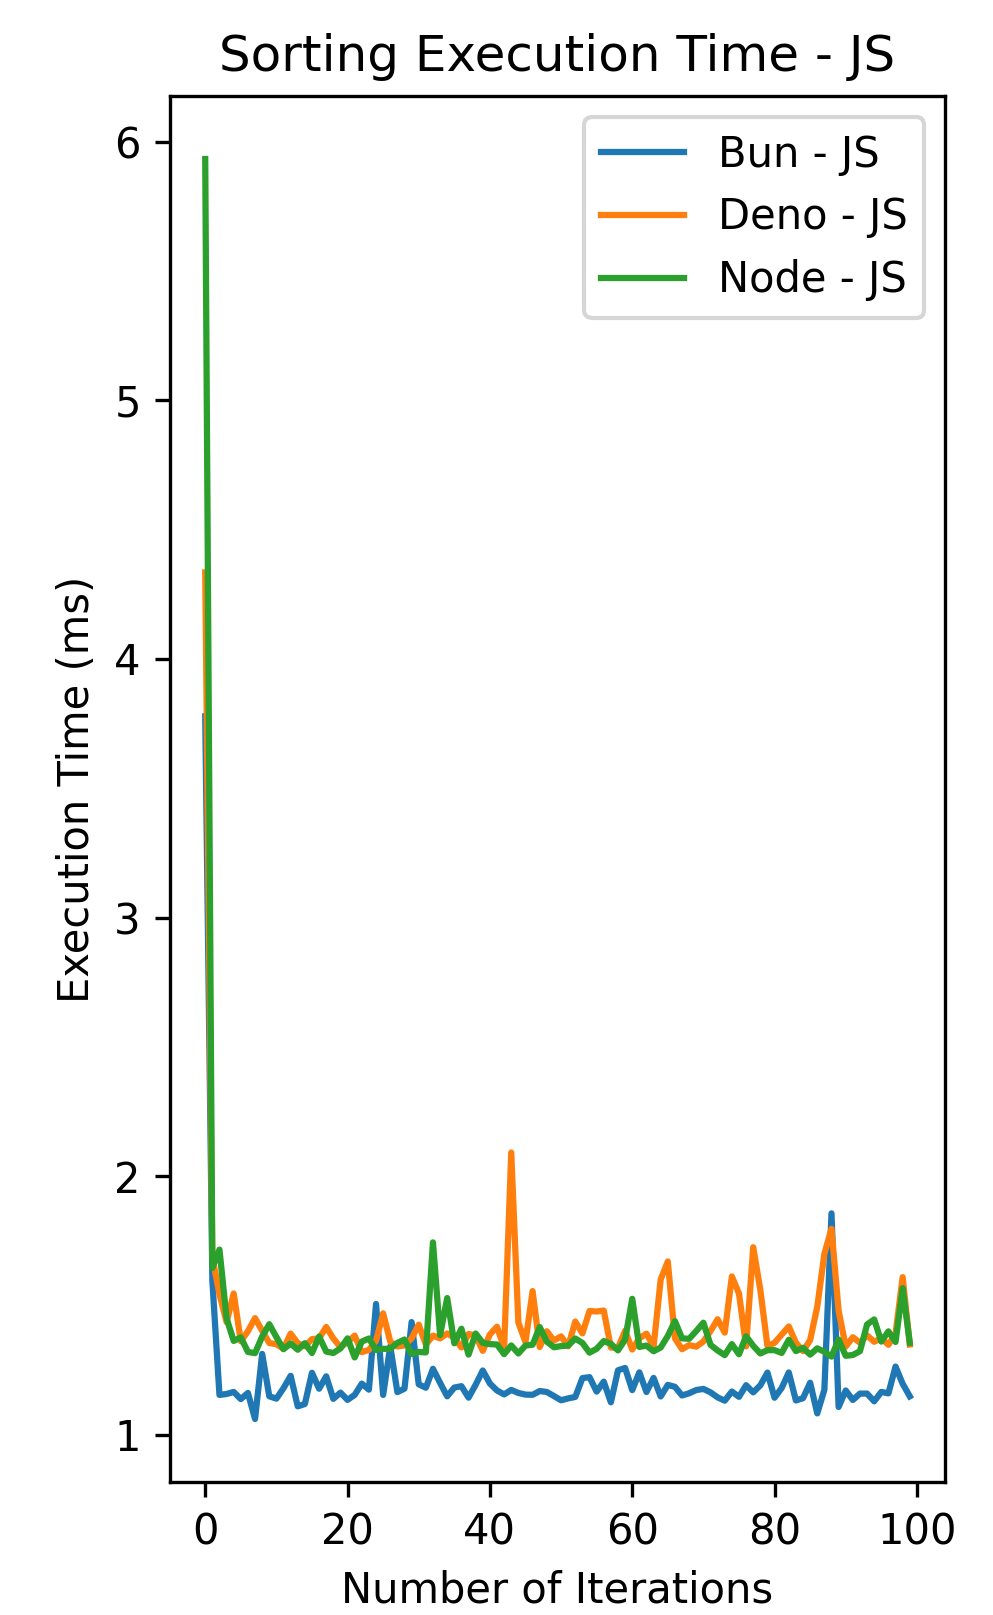
\includegraphics[width=\textwidth]{Figures/sorting/sorting_bubble_100_1000_js_time.png}
    \caption{Czas wykonania testu w milisekundach (ms)}
    \label{fig:bubble_sorting_e1_time}
  \end{subfigure}
  \begin{subfigure}[b]{0.42\textwidth}
    \centering
    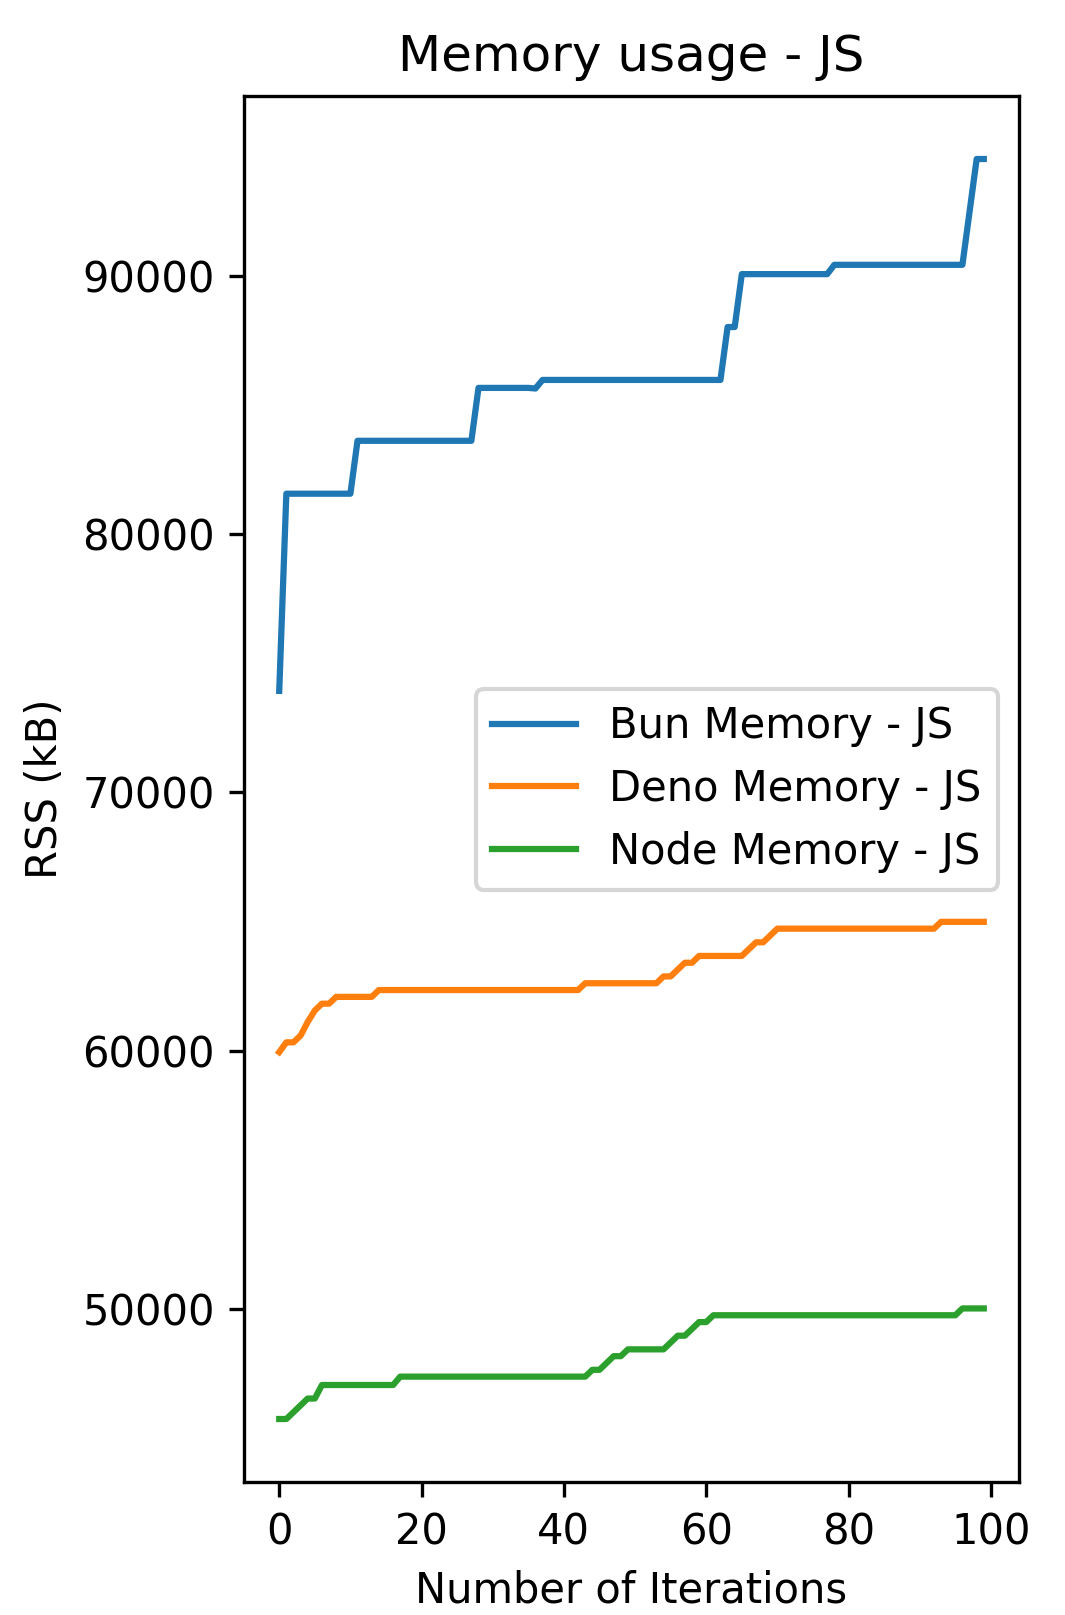
\includegraphics[width=\textwidth]{Figures/sorting/sorting_bubble_100_1000_js_memory.png}
    \caption{Zużycie pamięci operacyjnej w kilobajtach (kB)}
    \label{fig:bubble_sorting_e1_memory}
  \end{subfigure}
  \hfill
  \caption{Wyniki eksperymentów dla algorytmu sortowania bąbelkowego dla 100 iteracji i 1000 elementów - a) czas wykonania jednorazowego testu w milisekundach, b) ilość zajmowanej pamięci w kilobajtach (kB)}
  \label{fig:bubble_sorting_e1}
\end{figure}

Na wykresach \ref{fig:bubble_sorting_e1_time} możemy zauważyć, że czas wykonania w przypadku pierwszych 10 iteracji jest zwiększony w porównaniu do pozostałych próbek. Najprawdopodobniej jest to spowodowane tzw. rozgrzewaniem się środowiska, jest to zauważalne w przypadku środowiska NodeJS. Natomiast, z wykresu \ref{fig:bubble_sorting_e1_memory} możemy zauważyć tendencję wzrostową zużycia pamięci operacyjnej, największym zużyciem pamięci operacyjnej deklaruje środowisko Bun, które w ostatniej iteracji zużywa najwięcej ze wszystkich środowisk uruchomieniowych. 

Na rysunku \ref{fig:bubble_sorting_e1_ts} przedstawiono wyniki eksperymentów dla algorytmu sortowania bąbelkowego dla 100 iteracji i 1000 elementów napisanego w języku TypeScript. Na wykresach przedstawiono czas wykonania jednorazowego testu w milisekundach oraz ilość zajmowanej pamięci w kilobajtach (kB).

\begin{figure}[H]
  \centering
  \begin{subfigure}[b]{0.42\textwidth}
    \centering
    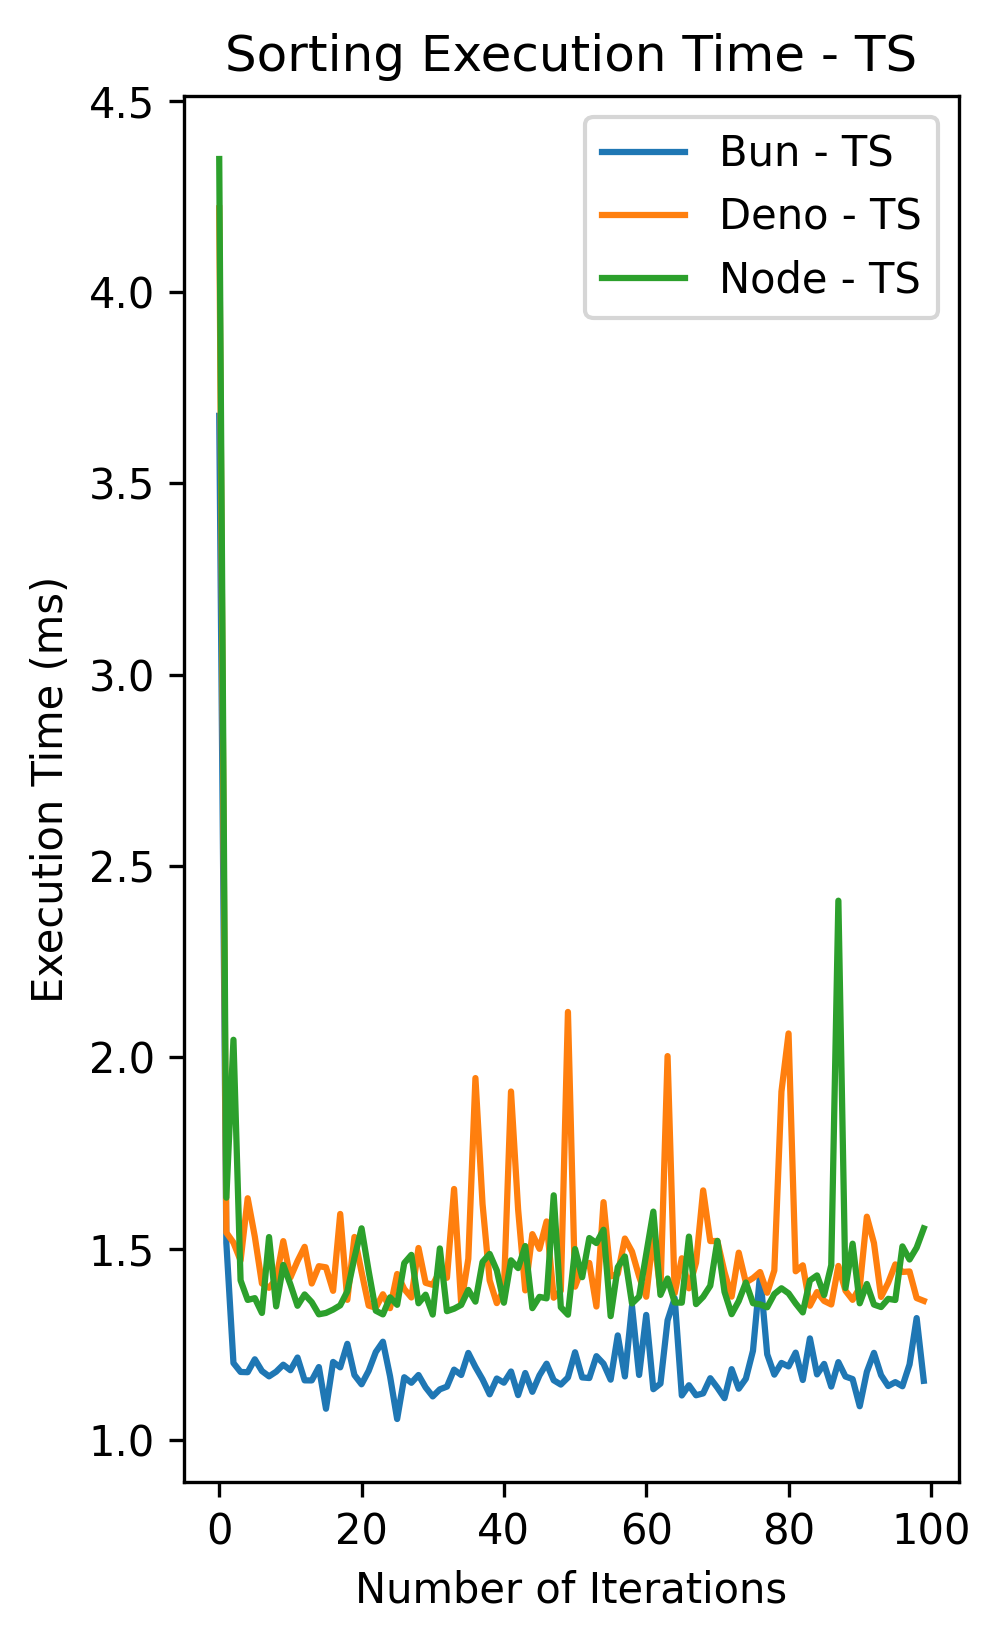
\includegraphics[width=\textwidth]{Figures/sorting/sorting_bubble_100_1000_ts_time.png}
    \caption{Czas wykonania testu w milisekundach (ms)}
    \label{fig:bubble_sorting_e1_ts_time}
  \end{subfigure}
  \begin{subfigure}[b]{0.42\textwidth}
    \centering
    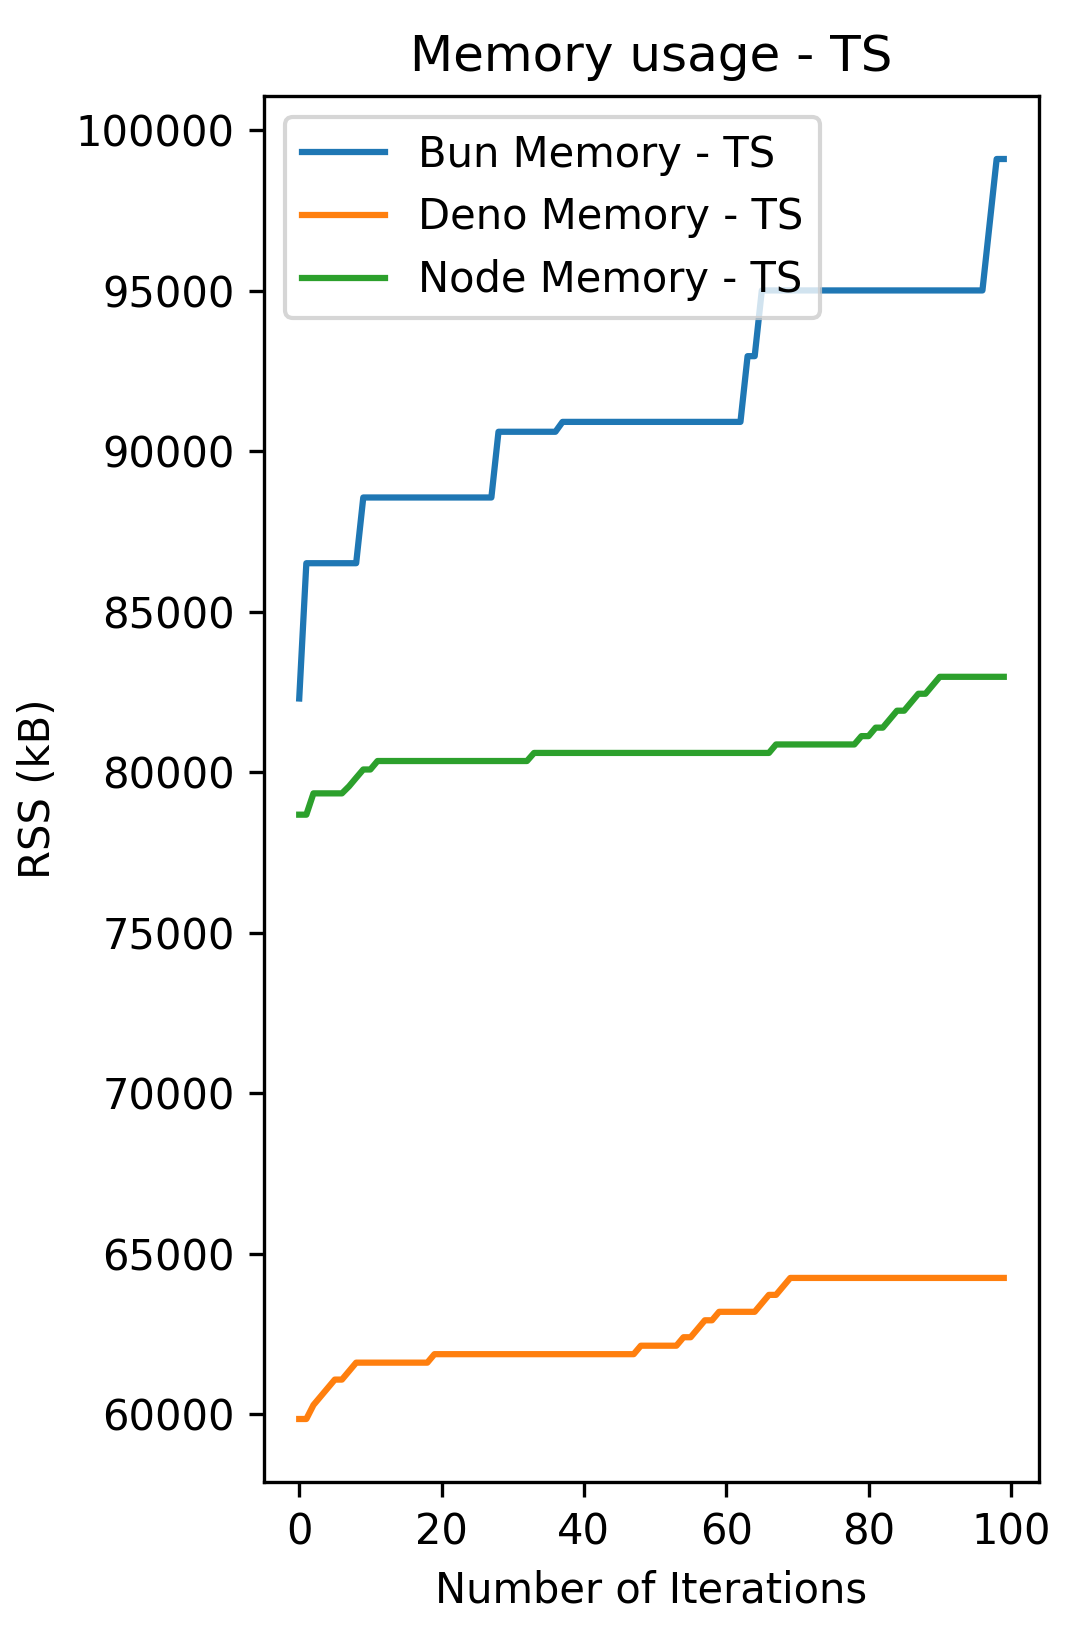
\includegraphics[width=\textwidth]{Figures/sorting/sorting_bubble_100_1000_ts_memory.png}
    \caption{Zużycie pamięci operacyjnej w kilobajtach (kB)}
    \label{fig:bubble_sorting_e1_ts_memory}
  \end{subfigure}
  \caption{Wyniki eksperymentów dla algorytmu sortowania bąbelkowego dla 100 iteracji i 1000 elementów - a) czas wykonania jednorazowego testu w milisekundach, b) ilość zajmowanej pamięci w kilobajtach (kB)}
  \label{fig:bubble_sorting_e1_ts}
\end{figure}

W porównaniu do wyników dla języka JavaScript, wyniki dla języka TypeScript są zbliżone. Na wykresach \ref{fig:bubble_sorting_e1_ts_time} możemy zauważyć, że czas wykonania w przypadku pierwszych 10 iteracji jest zwiększony w porównaniu do pozostałych próbek. Natomiast, z wykresu \ref{fig:bubble_sorting_e1_ts_memory} możemy zauważyć tendencję wzrostową zużycia pamięci operacyjnej, największym zużyciem pamięci operacyjnej deklaruje środowisko Bun, które w ostatniej iteracji zużywa najwięcej ze wszystkich środowisk uruchomieniowych.

Na rysunku \ref{fig:bubble_sorting_e2} przedstawiono wyniki eksperymentów dla algorytmu sortowania bąbelkowego dla 1000 iteracji i 1000 elementów napisanego w języku JavaScript. Na wykresach przedstawiono czas wykonania jednorazowego testu w milisekundach oraz ilość zajmowanej pamięci w kilobajtach (kB).

\begin{figure}[H]
  \centering
  \begin{subfigure}[b]{0.42\textwidth}
    \centering
    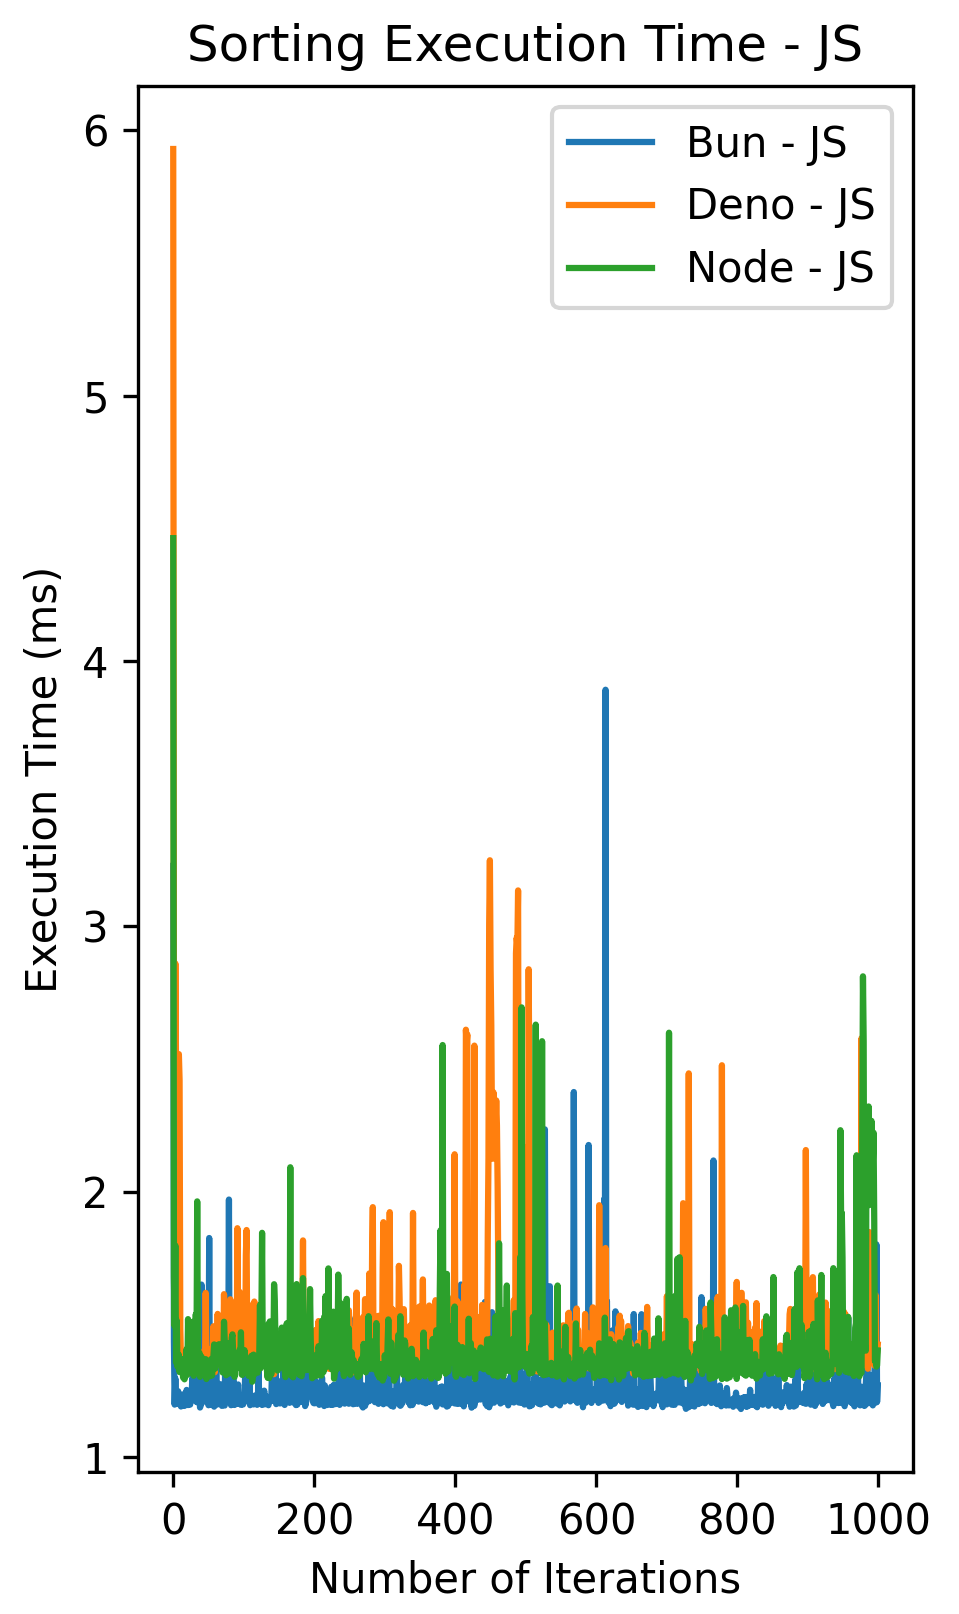
\includegraphics[width=\textwidth]{Figures/sorting/sorting_bubble_1000_1000_js_time.png}
    \caption{Czas wykonania testu w milisekundach (ms)}
    \label{fig:bubble_sorting_e2_time}
  \end{subfigure}
  \begin{subfigure}[b]{0.42\textwidth}
    \centering
    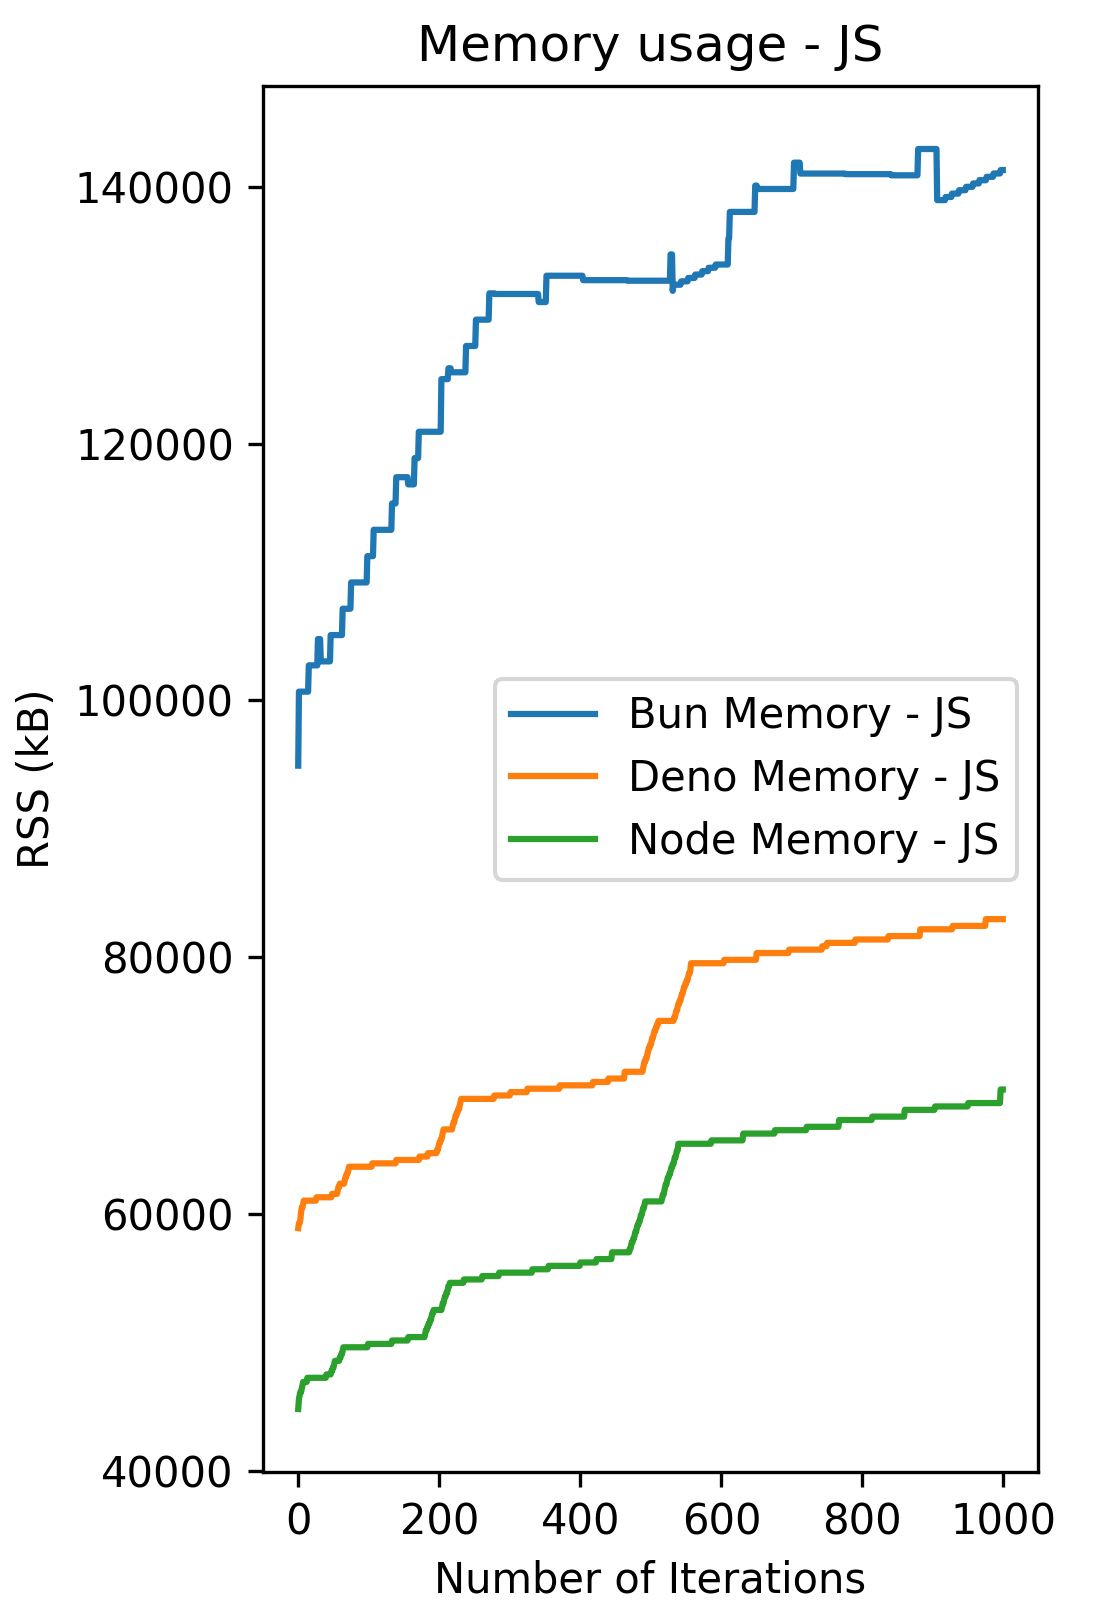
\includegraphics[width=\textwidth]{Figures/sorting/sorting_bubble_1000_1000_js_memory.png}
    \caption{Zużycie pamięci operacyjnej w kilobajtach (kB)}
    \label{fig:bubble_sorting_e2_memory}
  \end{subfigure}
  \caption{Wyniki eksperymentów dla algorytmu sortowania bąbelkowego dla 1000 iteracji i 1000 elementów dla języka JavaScript - a) czas wykonania jednorazowego testu w milisekundach, b) ilość zajmowanej pamięci w kilobajtach (kB)}
  \label{fig:bubble_sorting_e2}
\end{figure}

Przy zwiększonej ilości próbek możemy zauważyć na wykresach \ref{fig:bubble_sorting_e2_time}, że czas wykonania jest podobny względem wszystkich środowiska uruchomieniowych, Bun charakteryzuje się niższym czasem wykonania w porównaniu do pozostałych środowisk. Natomiast, z wykresu \ref{fig:bubble_sorting_e2_memory}, możemy także zauważyć, że Bun charakteryzuje się dużym zużyciem pamięci operacyjnej w porównaniu do pozostałych środowisk.

Na rysunku \ref{fig:bubble_sorting_e2_ts} przedstawiono wyniki eksperymentów dla algorytmu sortowania bąbelkowego dla 1000 iteracji i 10000 elementów napisanego w języku TypeScript. Na wykresach przedstawiono czas wykonania jednorazowego testu w milisekundach oraz ilość zajmowanej pamięci w kilobajtach (kB).

\begin{figure}[H]
  \centering
  \begin{subfigure}[b]{0.42\textwidth}
    \centering
    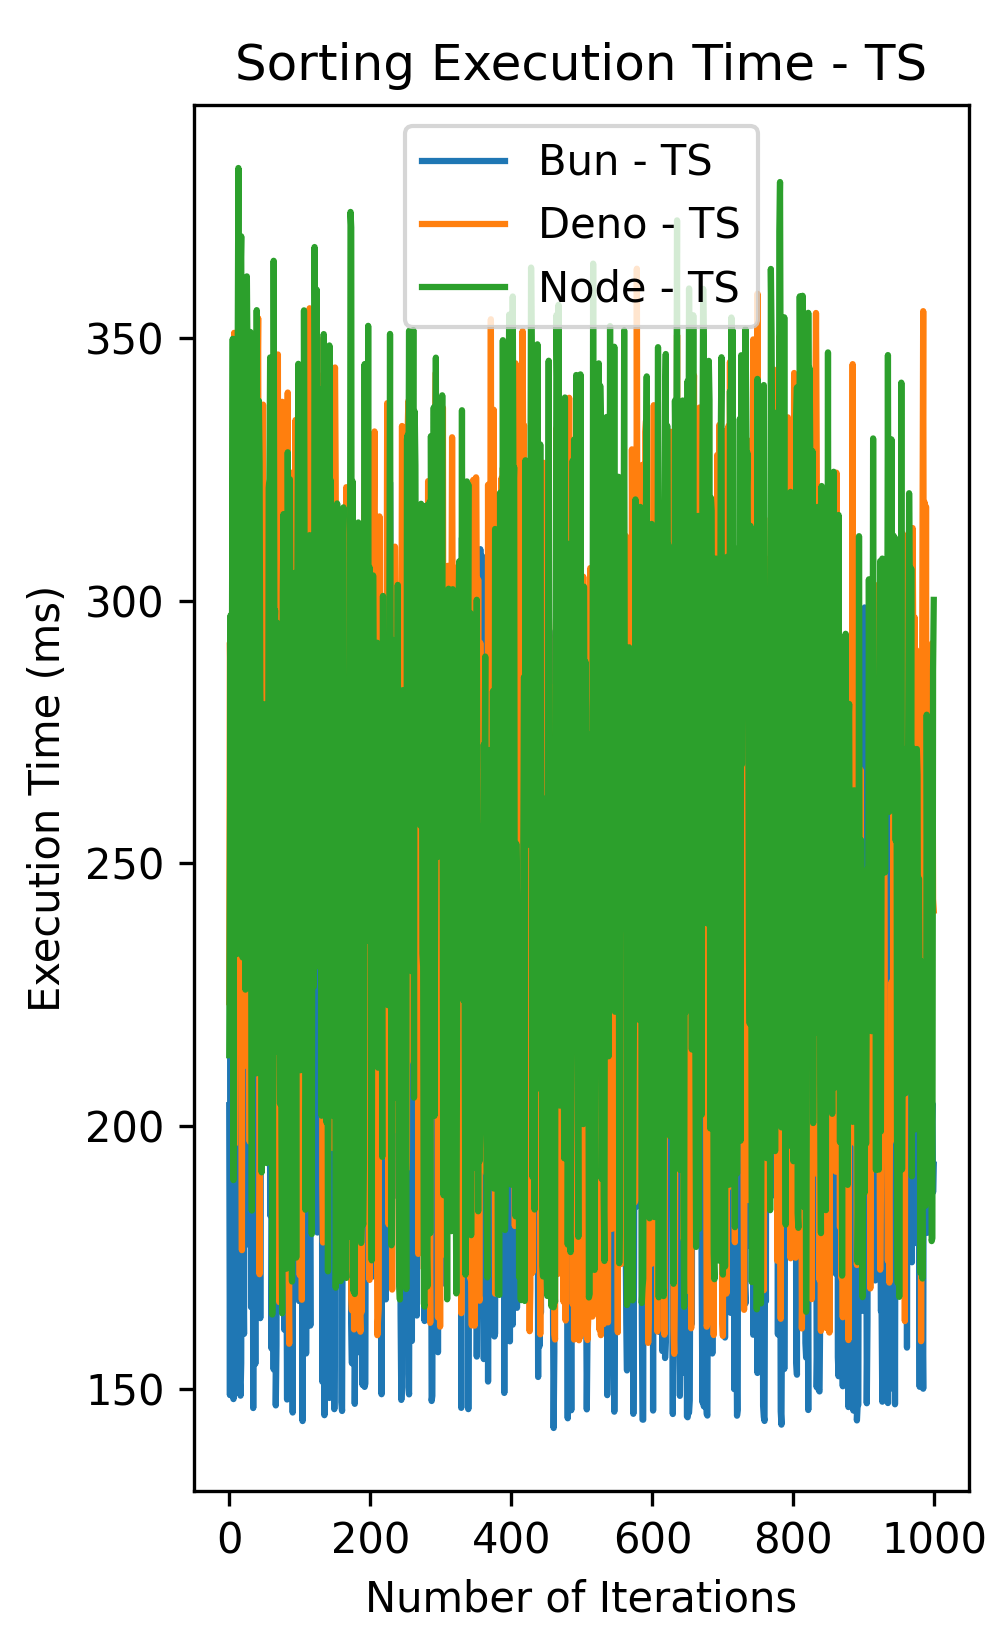
\includegraphics[width=\textwidth]{Figures/sorting/sorting_bubble_1000_10000_ts_time.png}
    \caption{Czas wykonania testu w milisekundach (ms)}
    \label{fig:bubble_sorting_e2_ts_time}
  \end{subfigure}
  \begin{subfigure}[b]{0.42\textwidth}
    \centering
    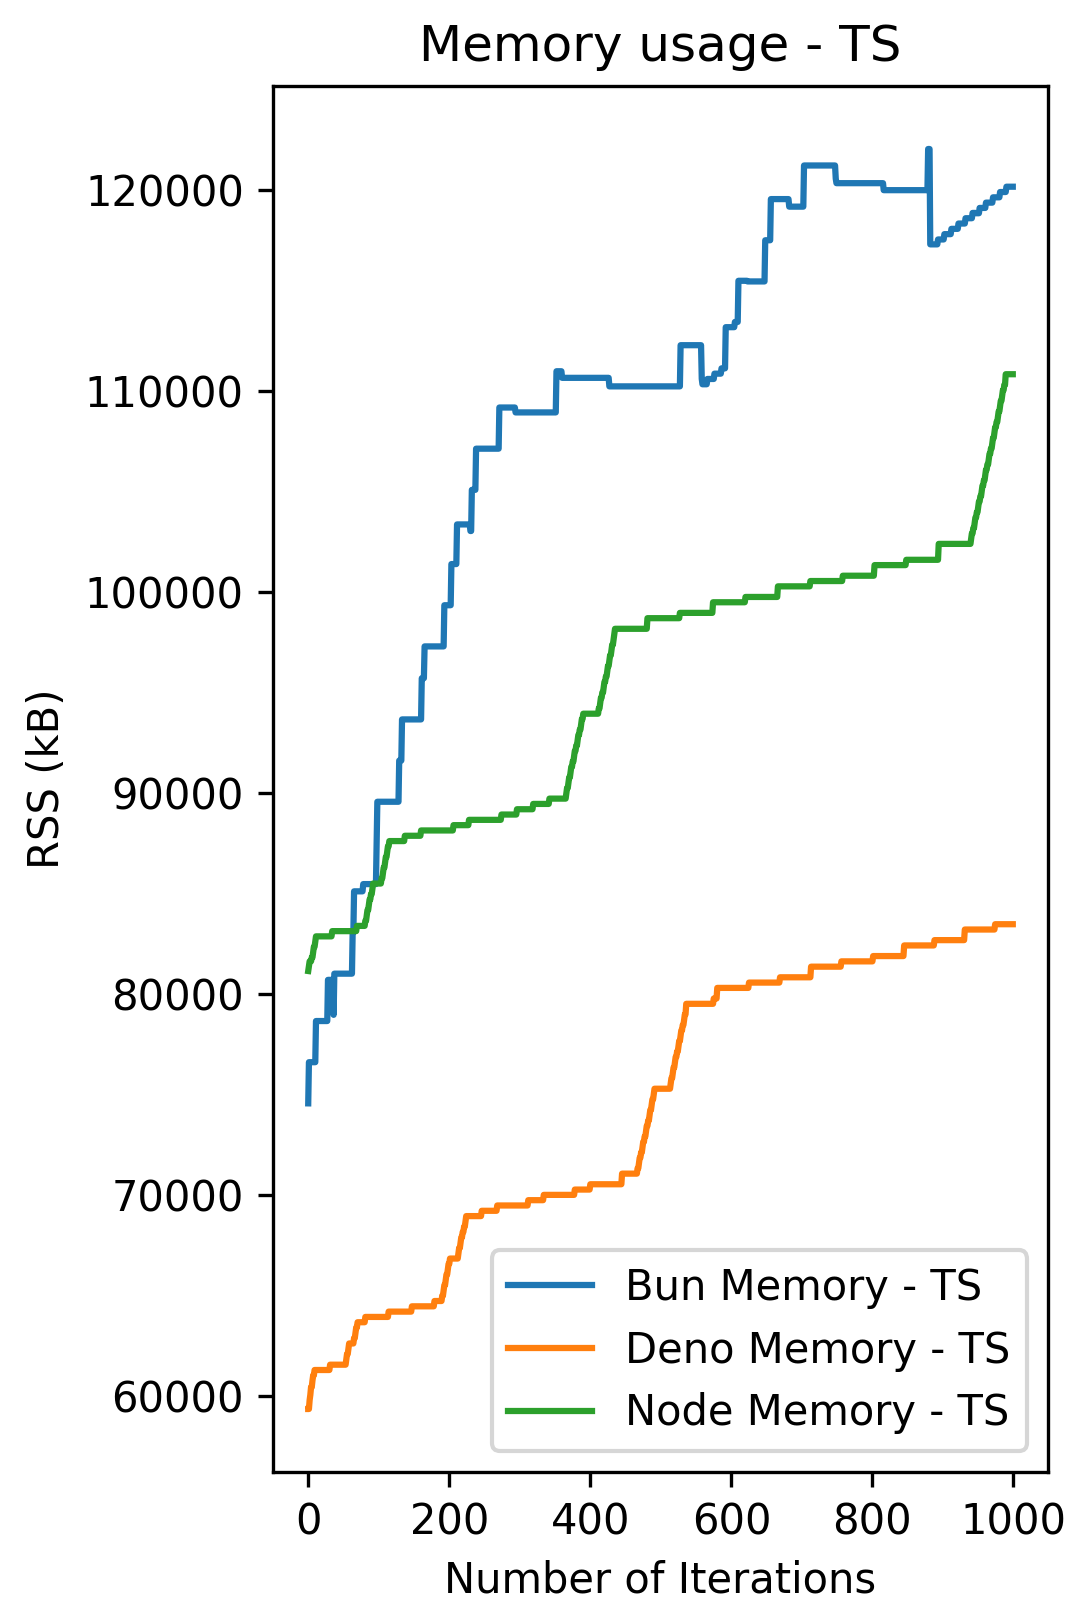
\includegraphics[width=\textwidth]{Figures/sorting/sorting_bubble_1000_1000_ts_memory.png}
    \caption{Zużycie pamięci operacyjnej w kilobajtach (kB)}
    \label{fig:bubble_sorting_e2_ts_memory}
  \end{subfigure}
  \caption{Wyniki eksperymentów dla algorytmu sortowania bąbelkowego dla 1000 iteracji i 1000 elementów dla języka TypeScript - a) czas wykonania jednorazowego testu w milisekundach, b) ilość zajmowanej pamięci w kilobajtach (kB)}
  \label{fig:bubble_sorting_e2_ts}
\end{figure}

W przypadku zwiększonej ilości próbek, na wykresach \ref{fig:bubble_sorting_e2_ts_time} możemy zauważyć, że czas wykonania wzrósł w porównaniu do poprzednich próbek. Wraz z zwiększeniem ilości próbek zwiększyło się zapotrzebowanie na pamięć operacyjną, co jest zauważalne na wykresach \ref{fig:bubble_sorting_e2_ts_memory}. Takie zachowanie środowisk może być spowodowane nieodpowiednim zarządzaniem przez środowiska pamięcią operacyjną.

Na rysunku \ref{fig:bubble_sorting_e3} przedstawiono wyniki eksperymentów dla algorytmu sortowania bąbelkowego dla 100 iteracji i 10000 elementów napisanego w języku JavaScript. Na wykresach przedstawiono czas wykonania jednorazowego testu w milisekundach oraz ilość zajmowanej pamięci w kilobajtach (kB).

\begin{figure}[H]
  \centering
  \begin{subfigure}[b]{0.42\textwidth}
    \centering
    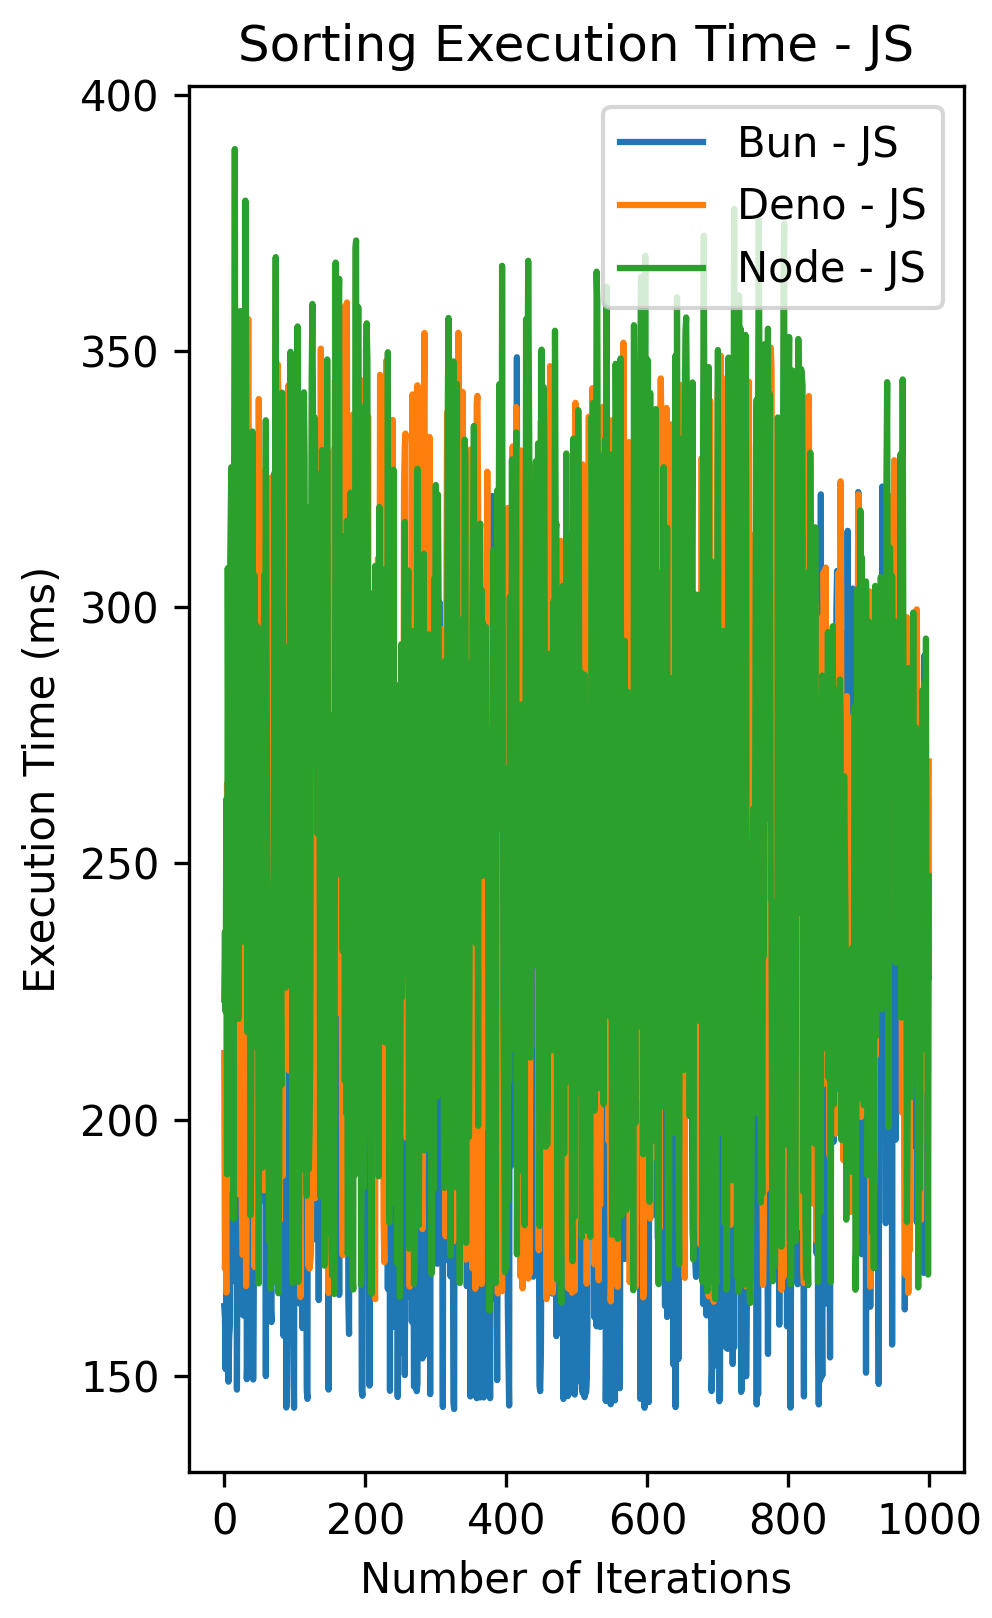
\includegraphics[width=\textwidth]{Figures/sorting/sorting_bubble_1000_10000_js_time.png}
    \caption{Czas wykonania testu w milisekundach (ms)}
    \label{fig:bubble_sorting_e3_time}
  \end{subfigure}
  \begin{subfigure}[b]{0.42\textwidth}
    \centering
    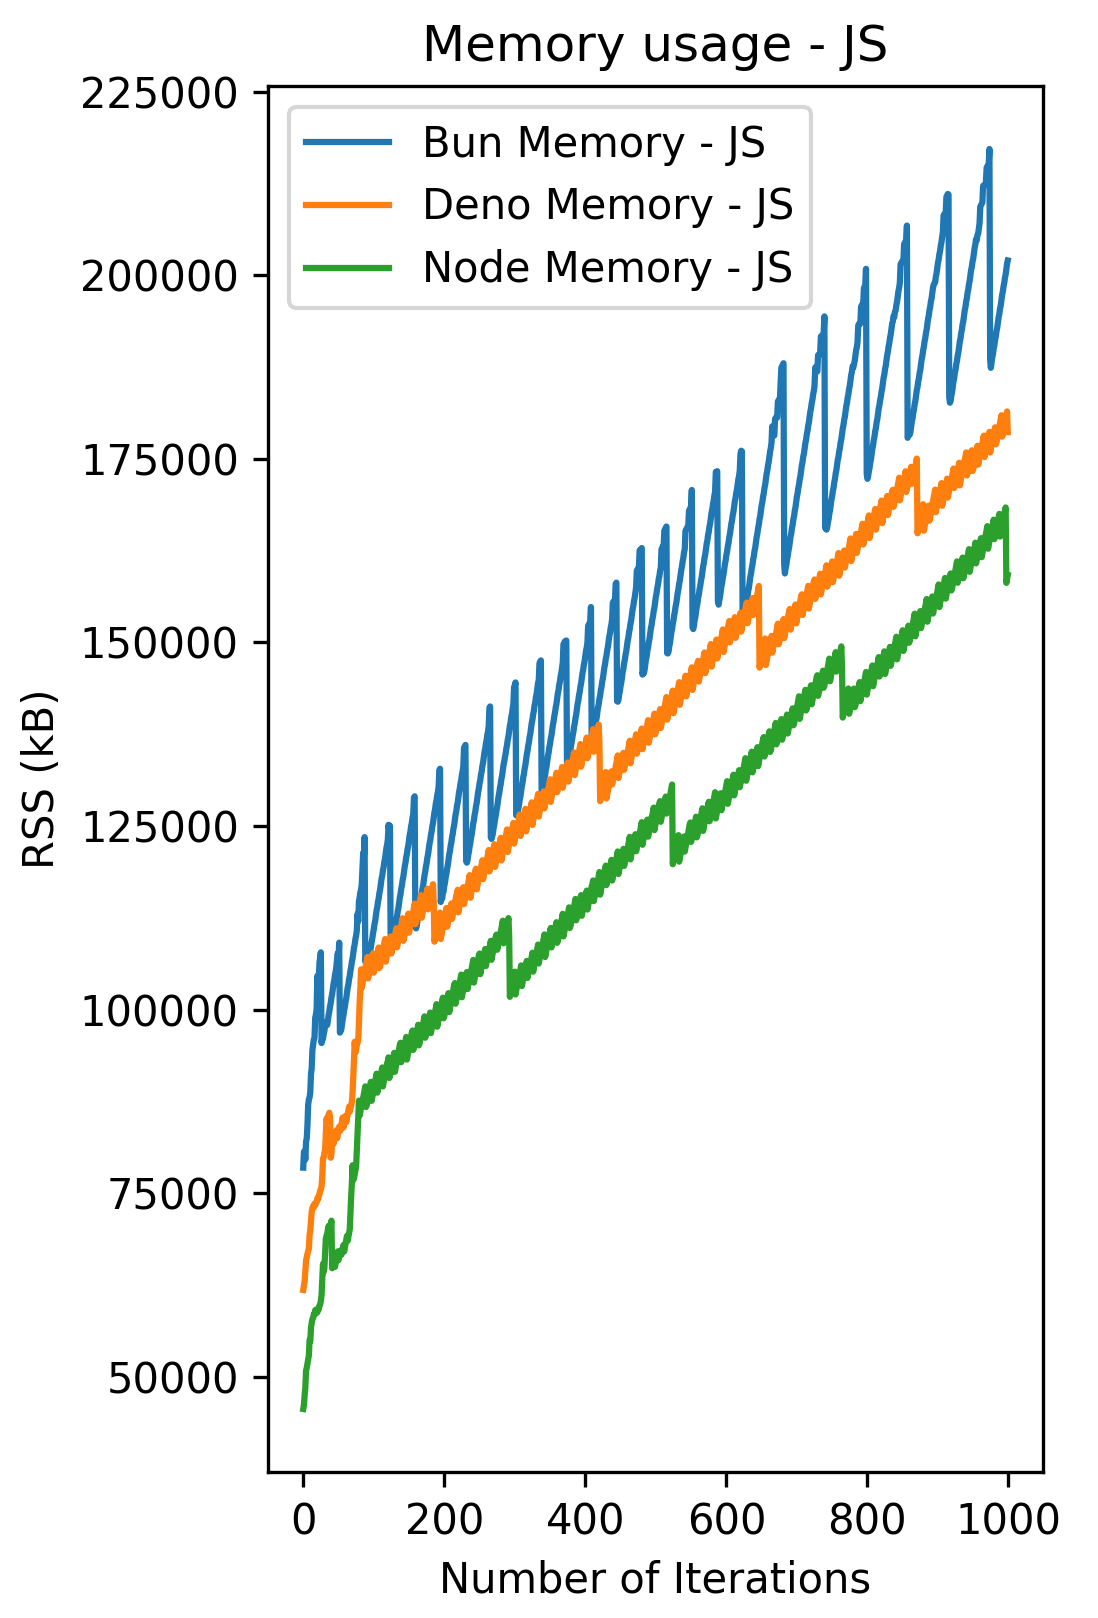
\includegraphics[width=\textwidth]{Figures/sorting/sorting_bubble_1000_10000_js_memory.png}
    \caption{Zużycie pamięci operacyjnej w kilobajtach (kB)}
    \label{fig:bubble_sorting_e3_memory}
  \end{subfigure}
  \caption{Wyniki eksperymentów dla algorytmu sortowania bąbelkowego dla 1000 iteracji i 10000 elementów dla języka JavaScript - a) czas wykonania jednorazowego testu w milisekundach, b) ilość zajmowanej pamięci w kilobajtach (kB)}
  \label{fig:bubble_sorting_e3}
\end{figure}

Na wykresach \ref{fig:bubble_sorting_e3_time} możemy zauważyć, że czas wykonania w przypadku pierwszych 10 iteracji jest zwiększony w porównaniu do pozostałych próbek. Natomiast, z wykresu \ref{fig:bubble_sorting_e3_memory} możemy zauważyć tendencję wzrostową zużycia pamięci operacyjnej, największym zużyciem pamięci operacyjnej deklaruje środowisko Bun, które w ostatniej iteracji zużywa najwięcej ze wszystkich środowisk uruchomieniowych. Momenty, w których zużycie pamięci spada może być spowodowane zwolnieniem pamięci operacyjnej przez środowisko za pomocą mechanizmu Garbage Collector.

Na rysunku \ref{fig:bubble_sorting_e3_ts} przedstawiono wyniki eksperymentów dla algorytmu sortowania bąbelkowego dla 100 iteracji i 10000 elementów napisanego w języku TypeScript. Na wykresach przedstawiono czas wykonania jednorazowego testu w milisekundach oraz ilość zajmowanej pamięci w kilobajtach (kB).

\begin{figure}[H]
  \centering
  \begin{subfigure}[b]{0.42\textwidth}
    \centering
    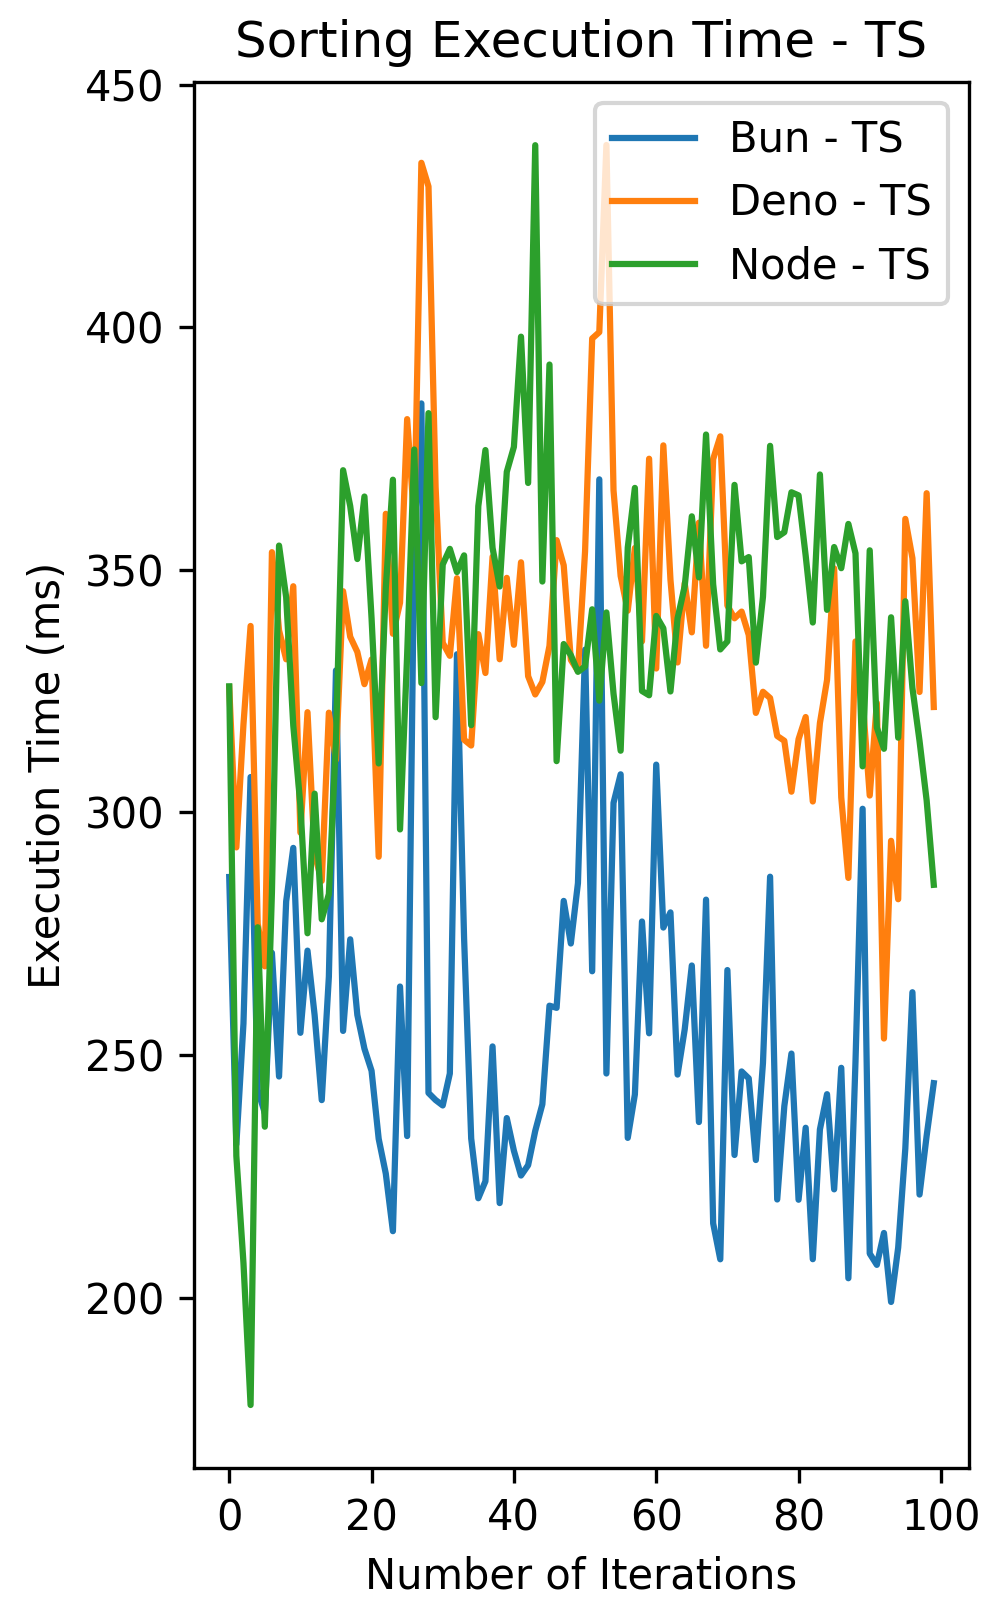
\includegraphics[width=\textwidth]{Figures/sorting/sorting_bubble_100_10000_ts_time.png}
    \caption{Czas wykonania testu w milisekundach (ms)}
    \label{fig:bubble_sorting_e3_ts_time}
  \end{subfigure}
  \begin{subfigure}[b]{0.42\textwidth}
    \centering
    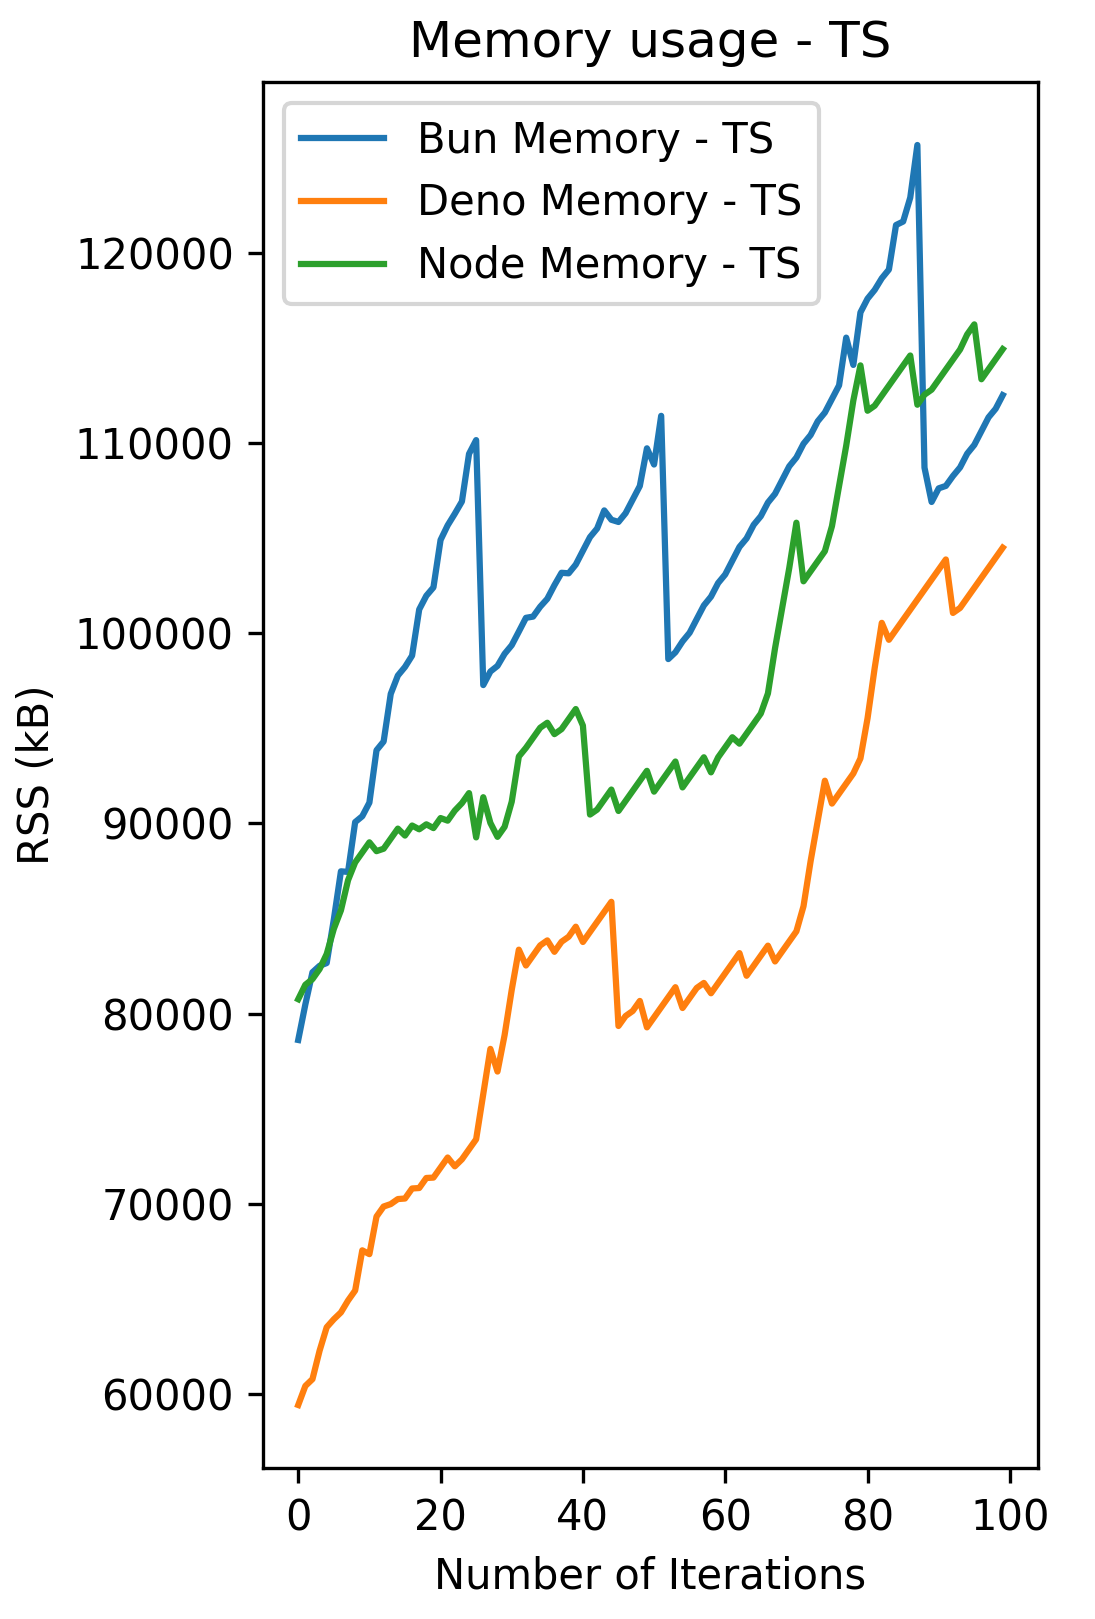
\includegraphics[width=\textwidth]{Figures/sorting/sorting_bubble_100_10000_ts_memory.png}
    \caption{Zużycie pamięci operacyjnej w kilobajtach (kB)}
    \label{fig:bubble_sorting_e3_ts_memory}
  \end{subfigure}
  \caption{Wyniki eksperymentów dla algorytmu sortowania bąbelkowego dla 1000 iteracji i 10000 elementów dla języka TypeScript - a) czas wykonania jednorazowego testu w milisekundach, b) ilość zajmowanej pamięci w kilobajtach (kB)}
  \label{fig:bubble_sorting_e3_ts}
\end{figure}

Na wykresach \ref{fig:bubble_sorting_e3_ts_time} możemy zauważyć, że czas wykonania w przypadku pierwszych 10 iteracji jest zwiększony w porównaniu do pozostałych próbek. Natomiast, z wykresu \ref{fig:bubble_sorting_e3_ts_memory} możemy zauważyć tendencję wzrostową zużycia pamięci operacyjnej, największym zużyciem pamięci operacyjnej deklaruje środowisko Bun, które w ostatniej iteracji zużywa najwięcej ze wszystkich środowisk uruchomieniowych.

Na rysunku \ref{fig:bubble_sorting_e4} przedstawiono wyniki eksperymentów dla algorytmu sortowania bąbelkowego dla 1000 iteracji i 1000 elementów napisanego w języku JavaScript. Na wykresach przedstawiono czas wykonania jednorazowego testu w milisekundach oraz ilość zajmowanej pamięci w kilobajtach (kB).

\begin{figure}[H]
  \centering
  \begin{subfigure}[b]{0.42\textwidth}
    \centering
    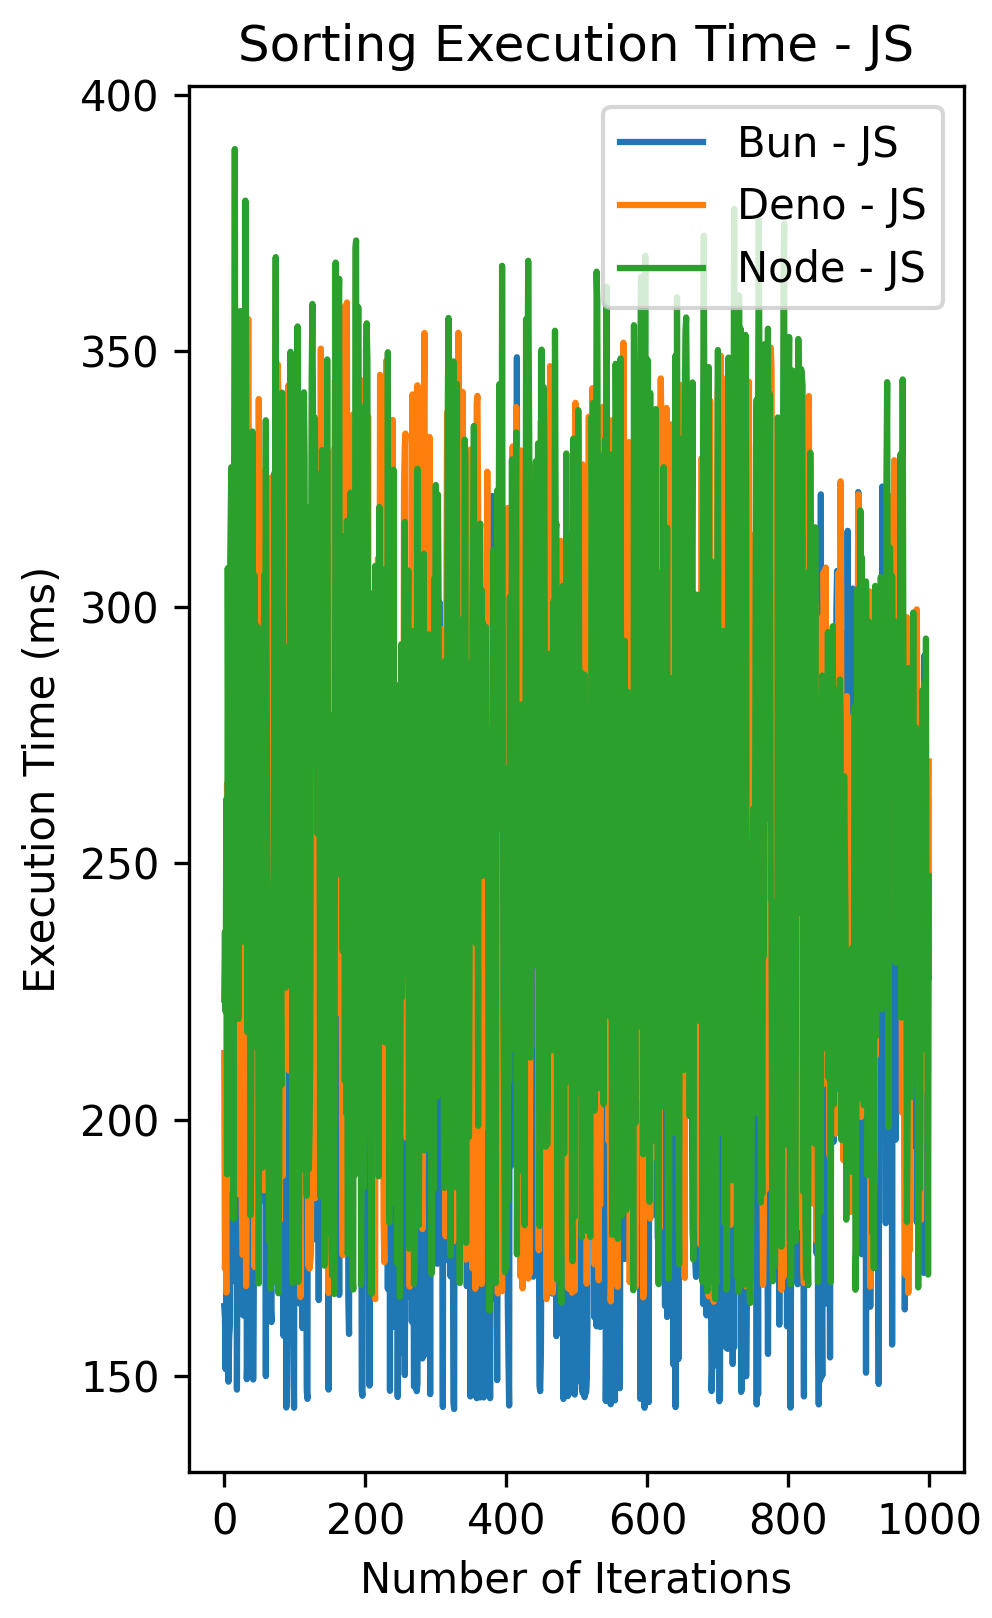
\includegraphics[width=\textwidth]{Figures/sorting/sorting_bubble_1000_10000_js_time.png}
    \caption{Czas wykonania testu w milisekundach (ms)}
    \label{fig:bubble_sorting_e4_time}
  \end{subfigure}
  \begin{subfigure}[b]{0.42\textwidth}
    \centering
    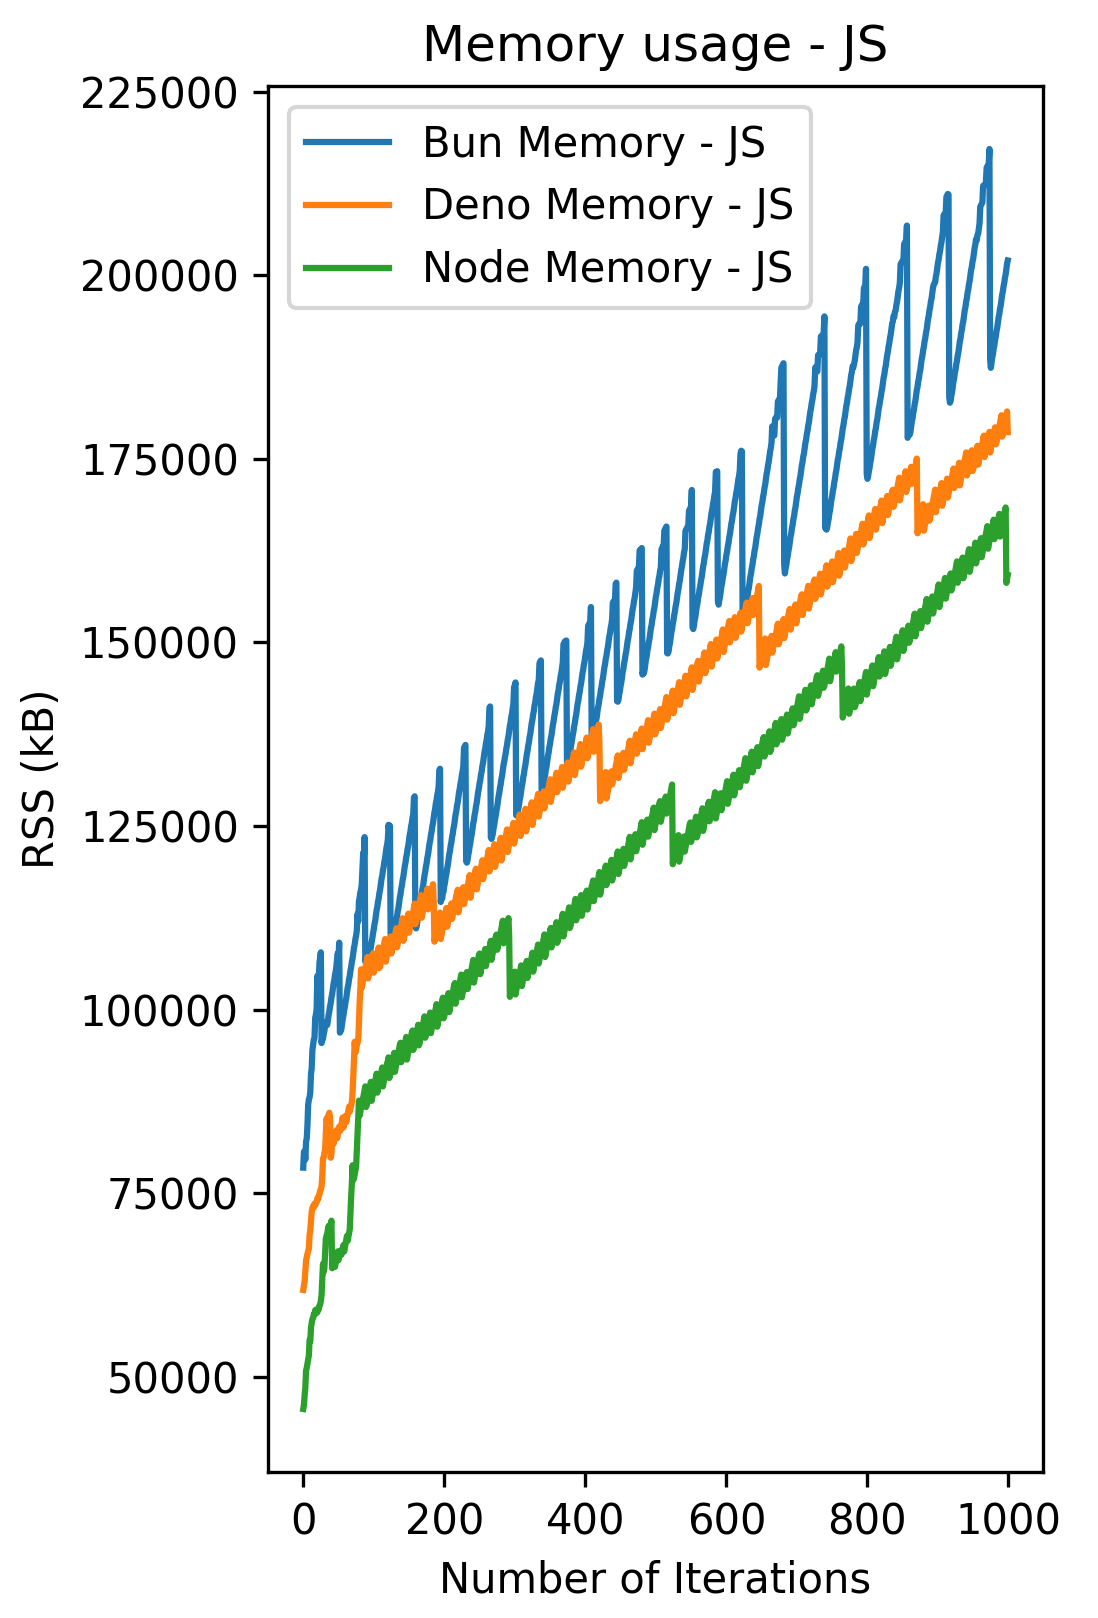
\includegraphics[width=\textwidth]{Figures/sorting/sorting_bubble_1000_10000_js_memory.png}
    \caption{Zużycie pamięci operacyjnej w kilobajtach (kB)}
    \label{fig:bubble_sorting_e4_memory}
  \end{subfigure}
  \caption{Wyniki eksperymentów dla algorytmu sortowania bąbelkowego dla 1000 iteracji i 10000 elementów dla języka JavaScript - a) czas wykonania jednorazowego testu w milisekundach, b) ilość zajmowanej pamięci w kilobajtach (kB)}
  \label{fig:bubble_sorting_e4}
\end{figure}

Na wykresach \ref{fig:bubble_sorting_e4_time} możemy zauważyć, że czas wykonania w przypadku pierwszych iteracji jest zwiększony w porównaniu do pozostałych próbek. Możemy także zauważyć, że środowisko NodeJS ma najdłuższy czas wykonania algorytmu w pierwszych iteracjach. Natomiast, z wykresu \ref{fig:bubble_sorting_e4_memory} możemy zauważyć tendencję wzrostową zużycia pamięci operacyjnej, największym zużyciem pamięci operacyjnej deklaruje środowisko Bun, które w ostatniej iteracji zużywa najwięcej ze wszystkich środowisk uruchomieniowych.

Na rysunku \ref{fig:bubble_sorting_e4_ts} przedstawiono wyniki eksperymentów dla algorytmu sortowania bąbelkowego dla 1000 iteracji i 10000 elementów napisanego w języku TypeScript. Na wykresach przedstawiono czas wykonania jednorazowego testu w milisekundach oraz ilość zajmowanej pamięci w kilobajtach (kB).

\begin{figure}[H]
  \centering
  \begin{subfigure}[b]{0.42\textwidth}
    \centering
    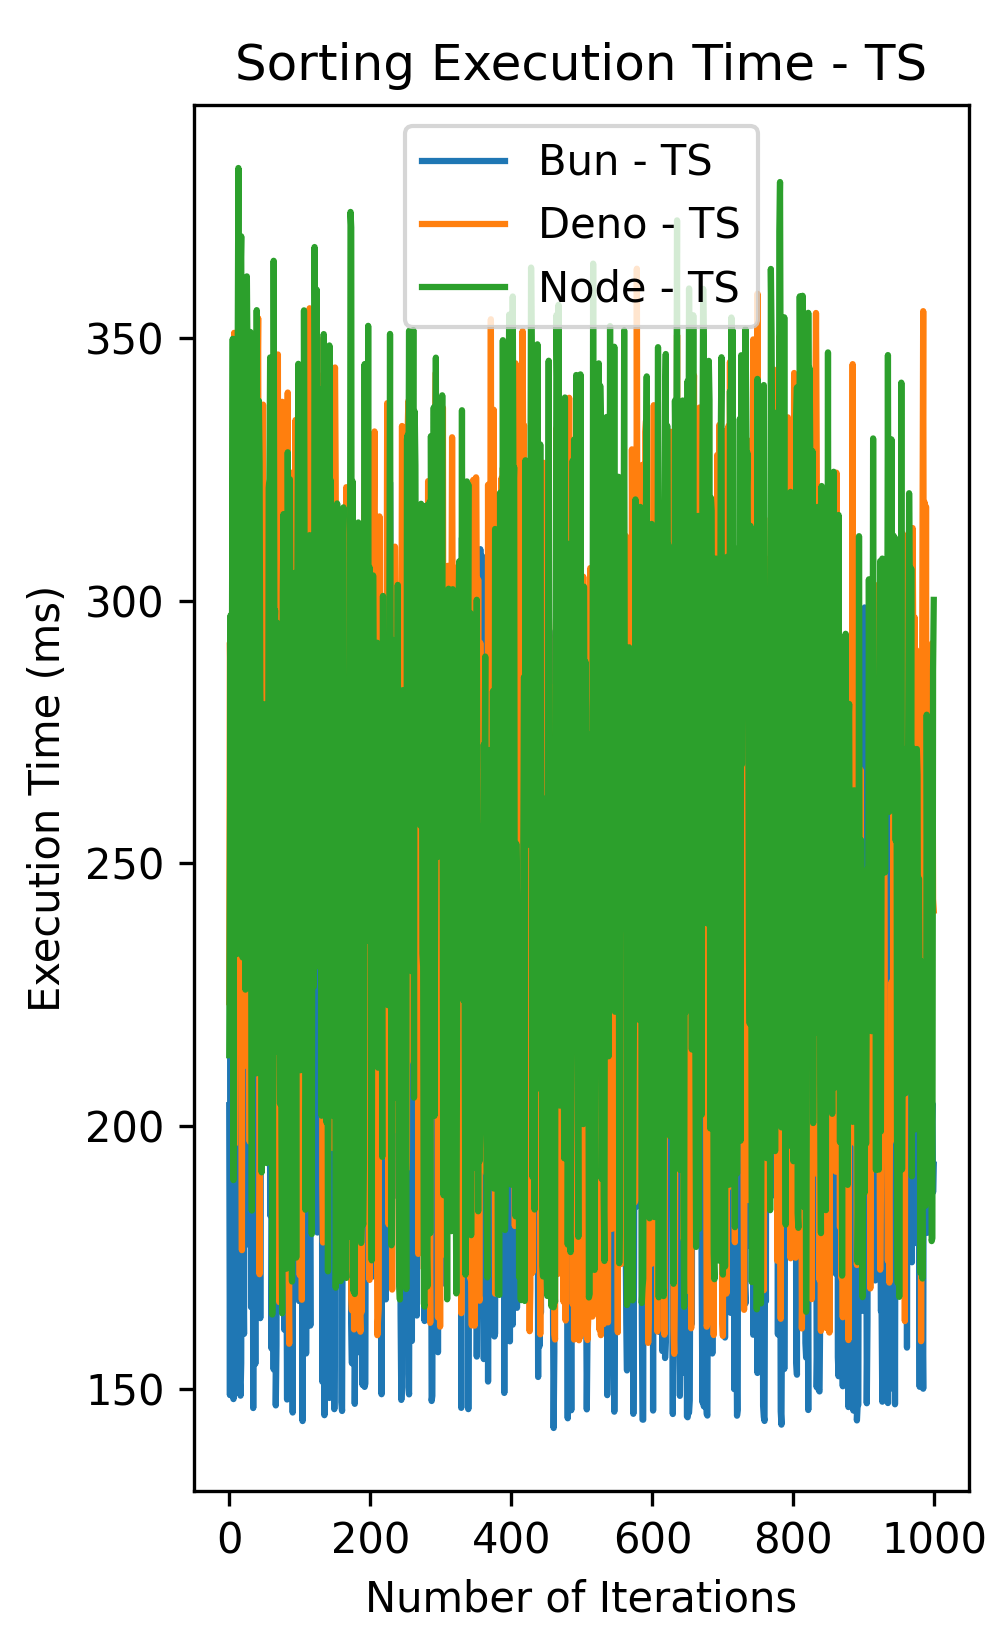
\includegraphics[width=\textwidth]{Figures/sorting/sorting_bubble_1000_10000_ts_time.png}
    \caption{Czas wykonania testu w milisekundach (ms)}
    \label{fig:bubble_sorting_e4_ts_time}
  \end{subfigure}
  \begin{subfigure}[b]{0.42\textwidth}
    \centering
    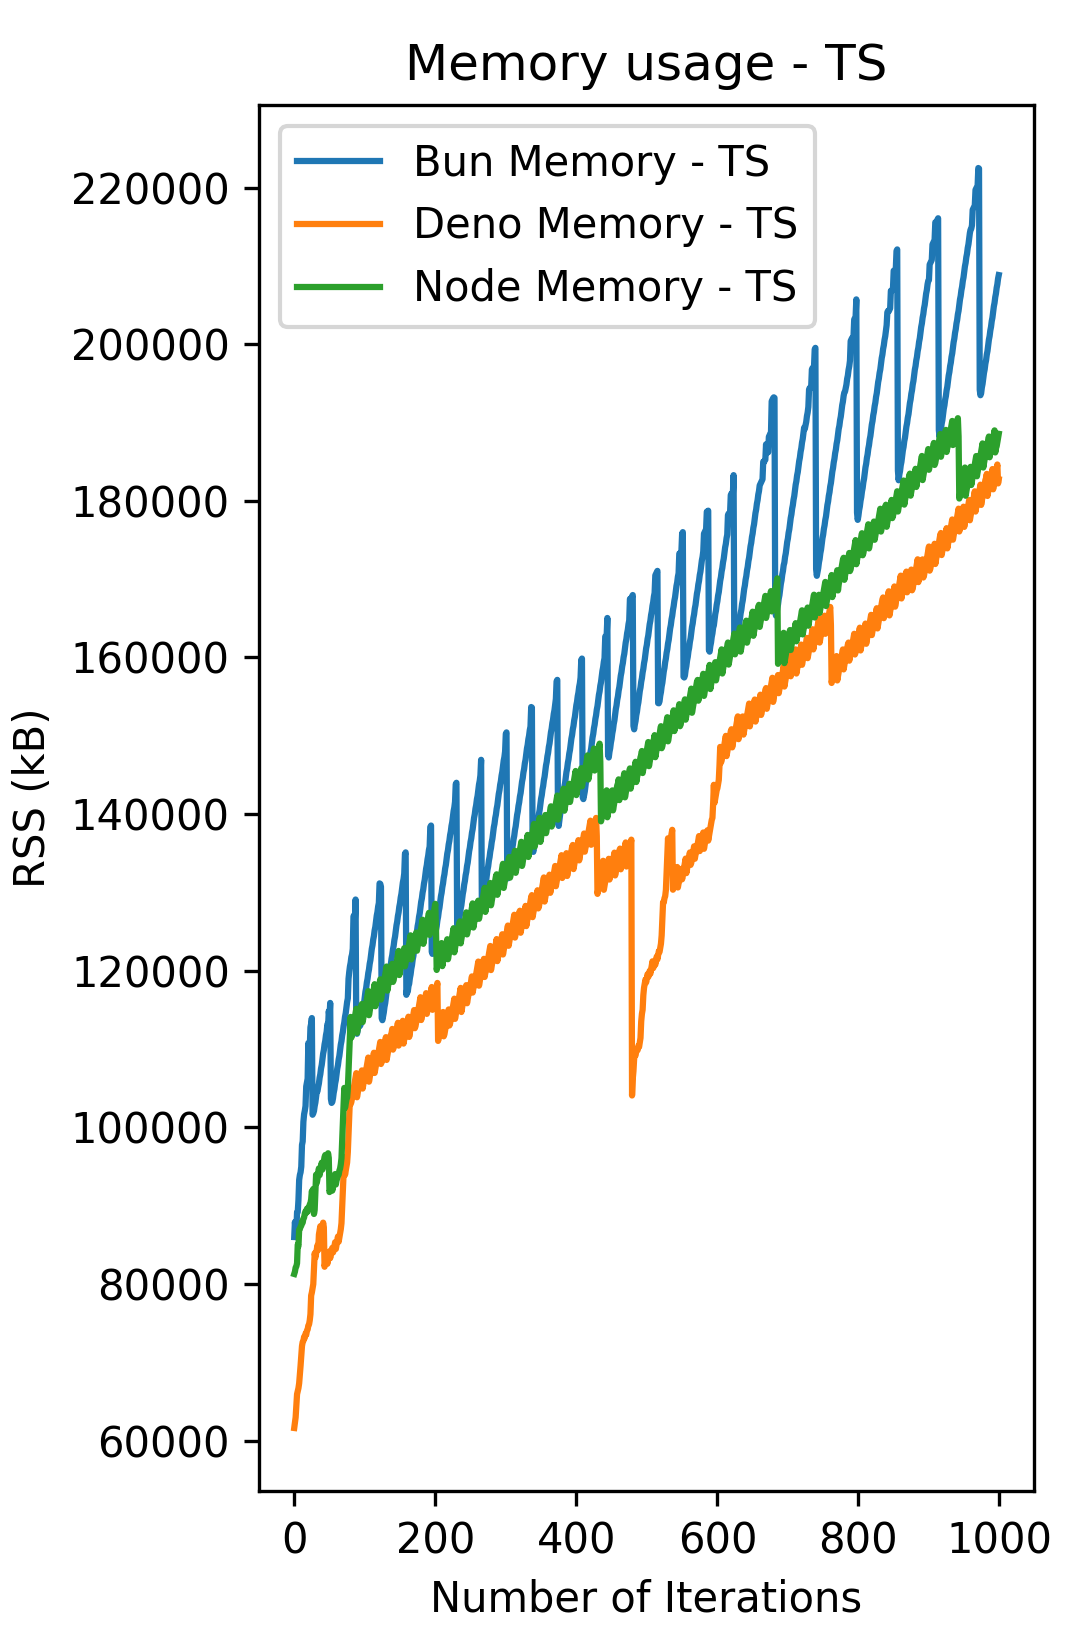
\includegraphics[width=\textwidth]{Figures/sorting/sorting_bubble_1000_10000_ts_memory.png}
    \caption{Zużycie pamięci operacyjnej w kilobajtach (kB)}
    \label{fig:bubble_sorting_e4_ts_memory}
  \end{subfigure}
  \caption{Wyniki eksperymentów dla algorytmu sortowania bąbelkowego dla 1000 iteracji i 10000 elementów dla języka TypeScript - a) czas wykonania jednorazowego testu w milisekundach, b) ilość zajmowanej pamięci w kilobajtach (kB)}
  \label{fig:bubble_sorting_e4_ts}
\end{figure}

Na rysunku \ref{fig:bubble_sorting_e4_ts_time} możemy zauważyć, że czas wykonania w przypadku pierwszych iteracji jest zwiększony w porównaniu do pozostałych próbek. Możemy także zauważyć, że środowisko NodeJS ma najdłuższy czas wykonania algorytmu w pierwszych iteracjach. Natomiast, z wykresu \ref{fig:bubble_sorting_e4_ts_memory} możemy zauważyć tendencję wzrostową zużycia pamięci operacyjnej, największym zużyciem pamięci operacyjnej deklaruje środowisko Bun, które w ostatniej iteracji zużywa najwięcej ze wszystkich środowisk uruchomieniowych.

\subsubsection{Wyniki - sortowanie szybkie}
Na rysunku \ref{fig:quick_sorting_e1} przedstawiono wyniki eksperymentów dla algorytmu sortowania szybkiego dla 100 iteracji i 1000 elementów napisanego w języku JavaScript. Na wykresach przedstawiono czas wykonania jednorazowego testu w milisekundach oraz ilość zajmowanej pamięci w kilobajtach (kB).

\begin{figure}[H]
  \centering
  \begin{subfigure}[b]{0.42\textwidth}
    \centering
    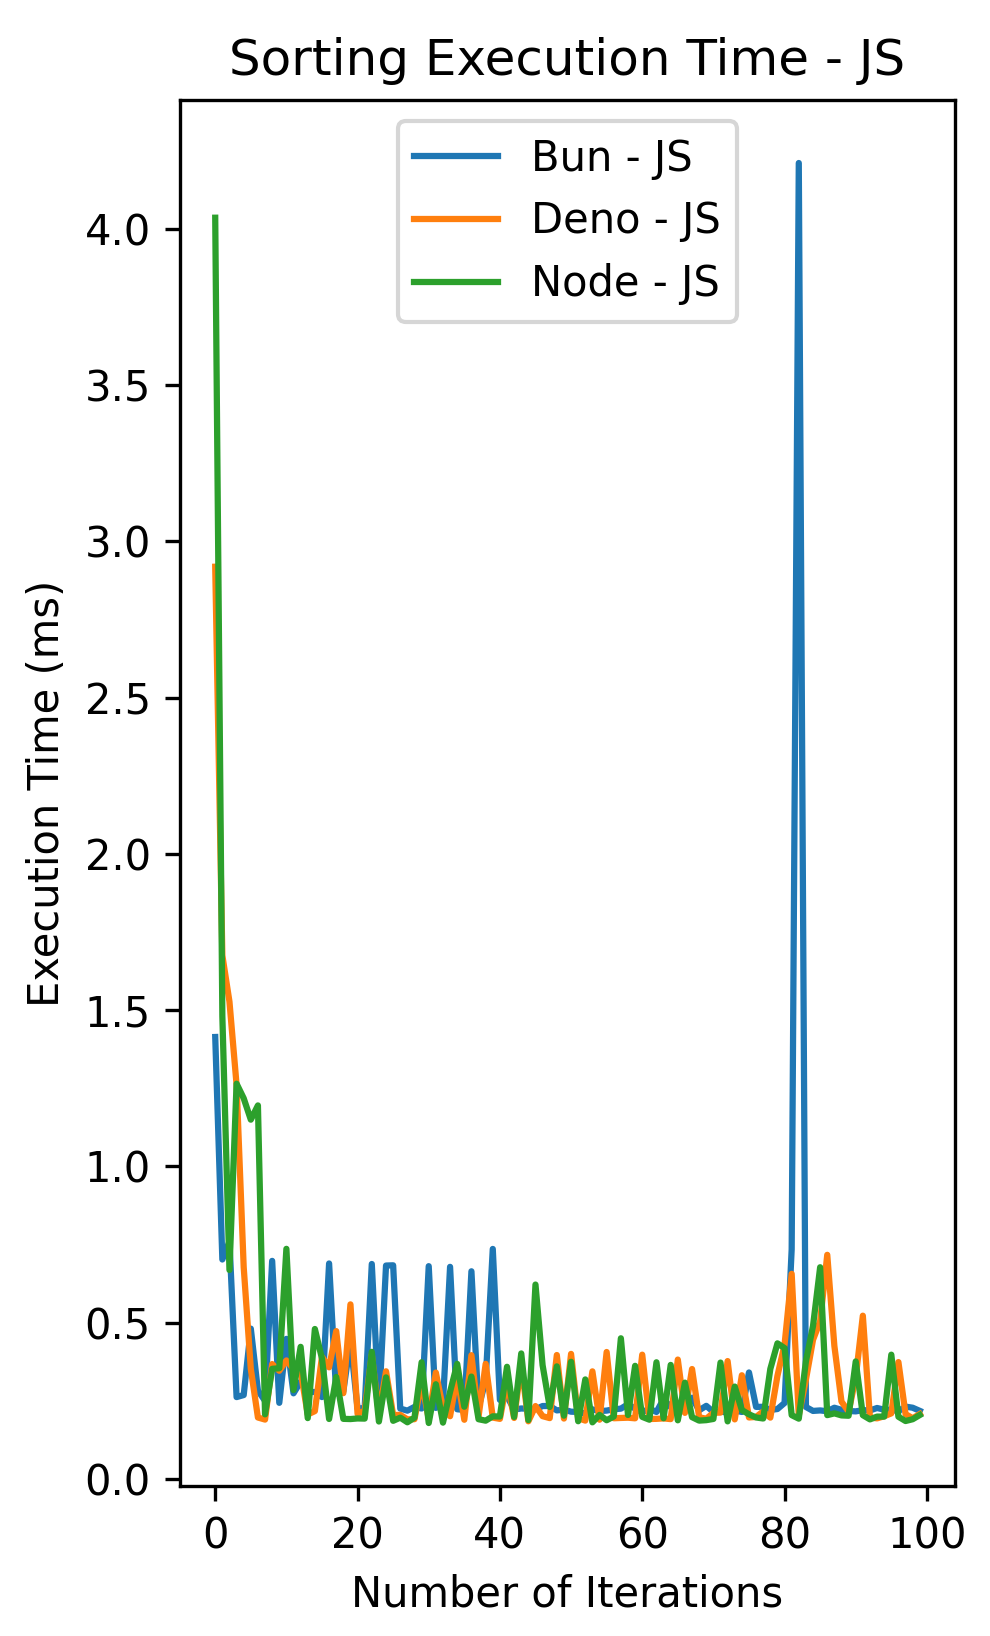
\includegraphics[width=\textwidth]{Figures/sorting/sorting_quick_100_1000_js_time.png}
    \caption{Czas wykonania testu w milisekundach (ms)}
    \label{fig:quick_sorting_e1_time}
  \end{subfigure}
  \begin{subfigure}[b]{0.42\textwidth}
    \centering
    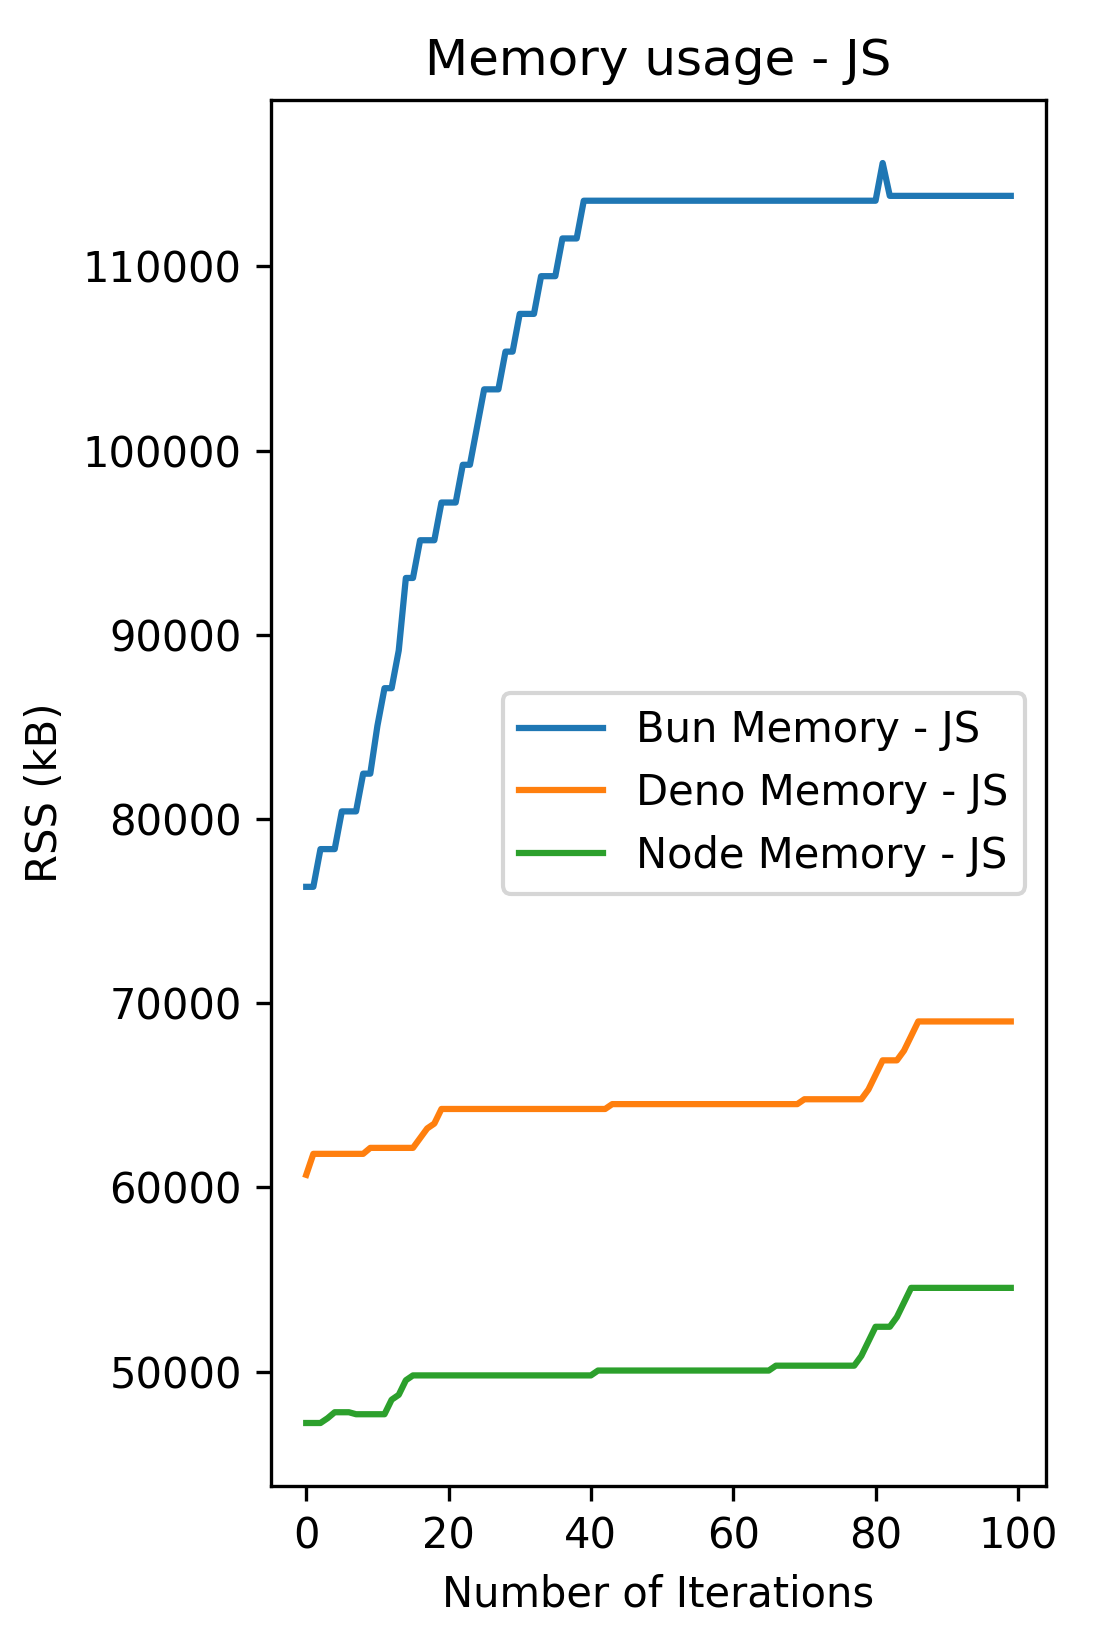
\includegraphics[width=\textwidth]{Figures/sorting/sorting_quick_100_1000_js_memory.png}
    \caption{Zużycie pamięci operacyjnej w kilobajtach (kB)}
    \label{fig:quick_sorting_e1_memory}
  \end{subfigure}
  \caption{Wyniki eksperymentów dla algorytmu sortowania szybkiego dla 100 iteracji i 1000 elementów - a) czas wykonania jednorazowego testu w milisekundach, b) ilość zajmowanej pamięci w kilobajtach (kB)}
  \label{fig:quick_sorting_e1}
\end{figure}

Na wykresie \ref{fig:quick_sorting_e1_time} możemy zauważyć, że czas wykonania w przypadku pierwszych 10 iteracji jest zwiększony w porównaniu do pozostałych próbek. Natomiast, z wykresu \ref{fig:quick_sorting_e1_memory} możemy zauważyć tendencję wzrostową zużycia pamięci operacyjnej, największym zużyciem pamięci operacyjnej deklaruje środowisko Bun, które w ostatniej iteracji zużywa najwięcej ze wszystkich środowisk uruchomieniowych.

Na rysunku \ref{fig:quick_sorting_e1_ts} przedstawiono wyniki eksperymentów dla algorytmu sortowania szybkiego dla 100 iteracji i 1000 elementów napisanego w języku TypeScript. Na wykresach przedstawiono czas wykonania jednorazowego testu w milisekundach oraz ilość zajmowanej pamięci w kilobajtach (kB).

\begin{figure}[H]
  \centering
  \begin{subfigure}[b]{0.42\textwidth}
    \centering
    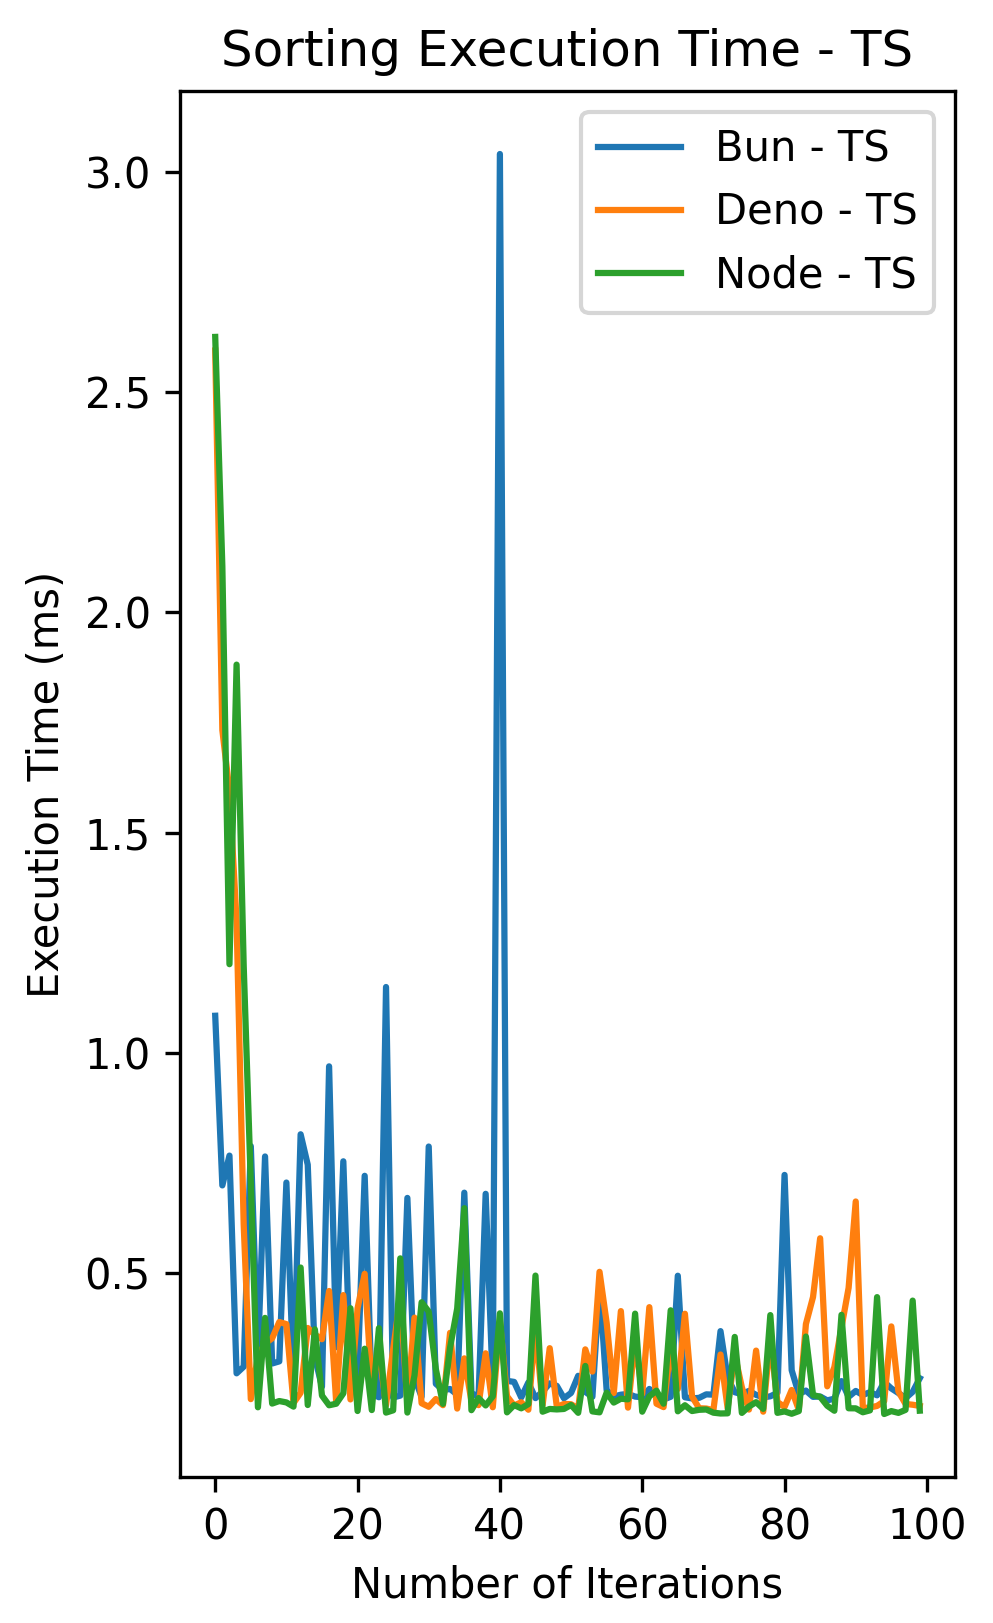
\includegraphics[width=\textwidth]{Figures/sorting/sorting_quick_100_1000_ts_time.png}
    \caption{Czas wykonania testu w milisekundach (ms)}
    \label{fig:quick_sorting_e1_tsquick_sorting_e1_time}
  \end{subfigure}
  \begin{subfigure}[b]{0.42\textwidth}
    \centering
    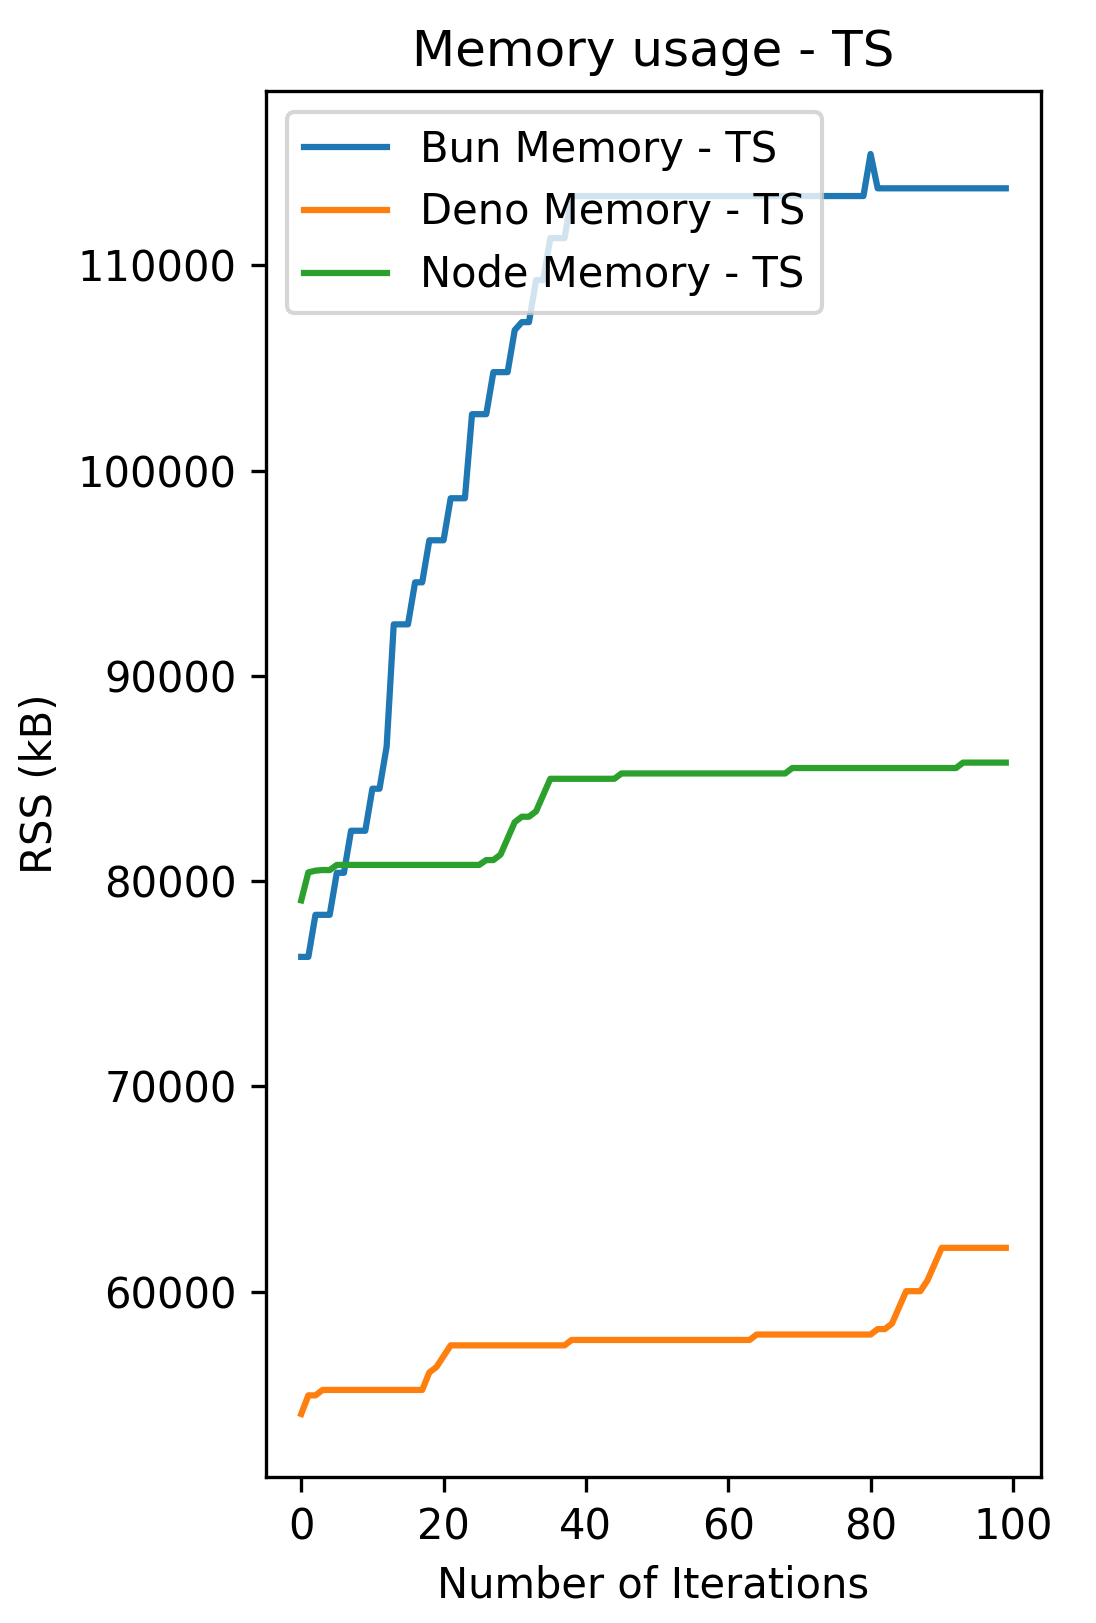
\includegraphics[width=\textwidth]{Figures/sorting/sorting_quick_100_1000_ts_memory.png}
    \caption{Zużycie pamięci operacyjnej w kilobajtach (kB)}
    \label{fig:quick_sorting_e1_ts_memory}
  \end{subfigure}
  \caption{Wyniki eksperymentów dla algorytmu sortowania szybkiego dla 100 iteracji i 1000 elementów - a) czas wykonania jednorazowego testu w milisekundach, b) ilość zajmowanej pamięci w kilobajtach (kB)}
  \label{fig:quick_sorting_e1_ts}
\end{figure}

Na rysunku \ref{fig:quick_sorting_e1_time} możemy zauważyć, że czas wykonania w przypadku pierwszych 10 iteracji jest zwiększony w porównaniu do pozostałych próbek. Natomiast, z wykresu \ref{fig:quick_sorting_e1_memory} możemy zauważyć tendencję wzrostową zużycia pamięci operacyjnej, największym zużyciem pamięci operacyjnej deklaruje środowisko Bun, które w ostatniej iteracji zużywa najwięcej ze wszystkich środowisk uruchomieniowych.

Na rysunku \ref{fig:quick_sorting_e2} przedstawiono wyniki eksperymentów dla algorytmu sortowania szybkiego dla 1000 iteracji i 1000 elementów napisanego w języku JavaScript. Na wykresach przedstawiono czas wykonania jednorazowego testu w milisekundach oraz ilość zajmowanej pamięci w kilobajtach (kB).

\begin{figure}[H]
  \centering
  \begin{subfigure}[b]{0.42\textwidth}
    \centering
    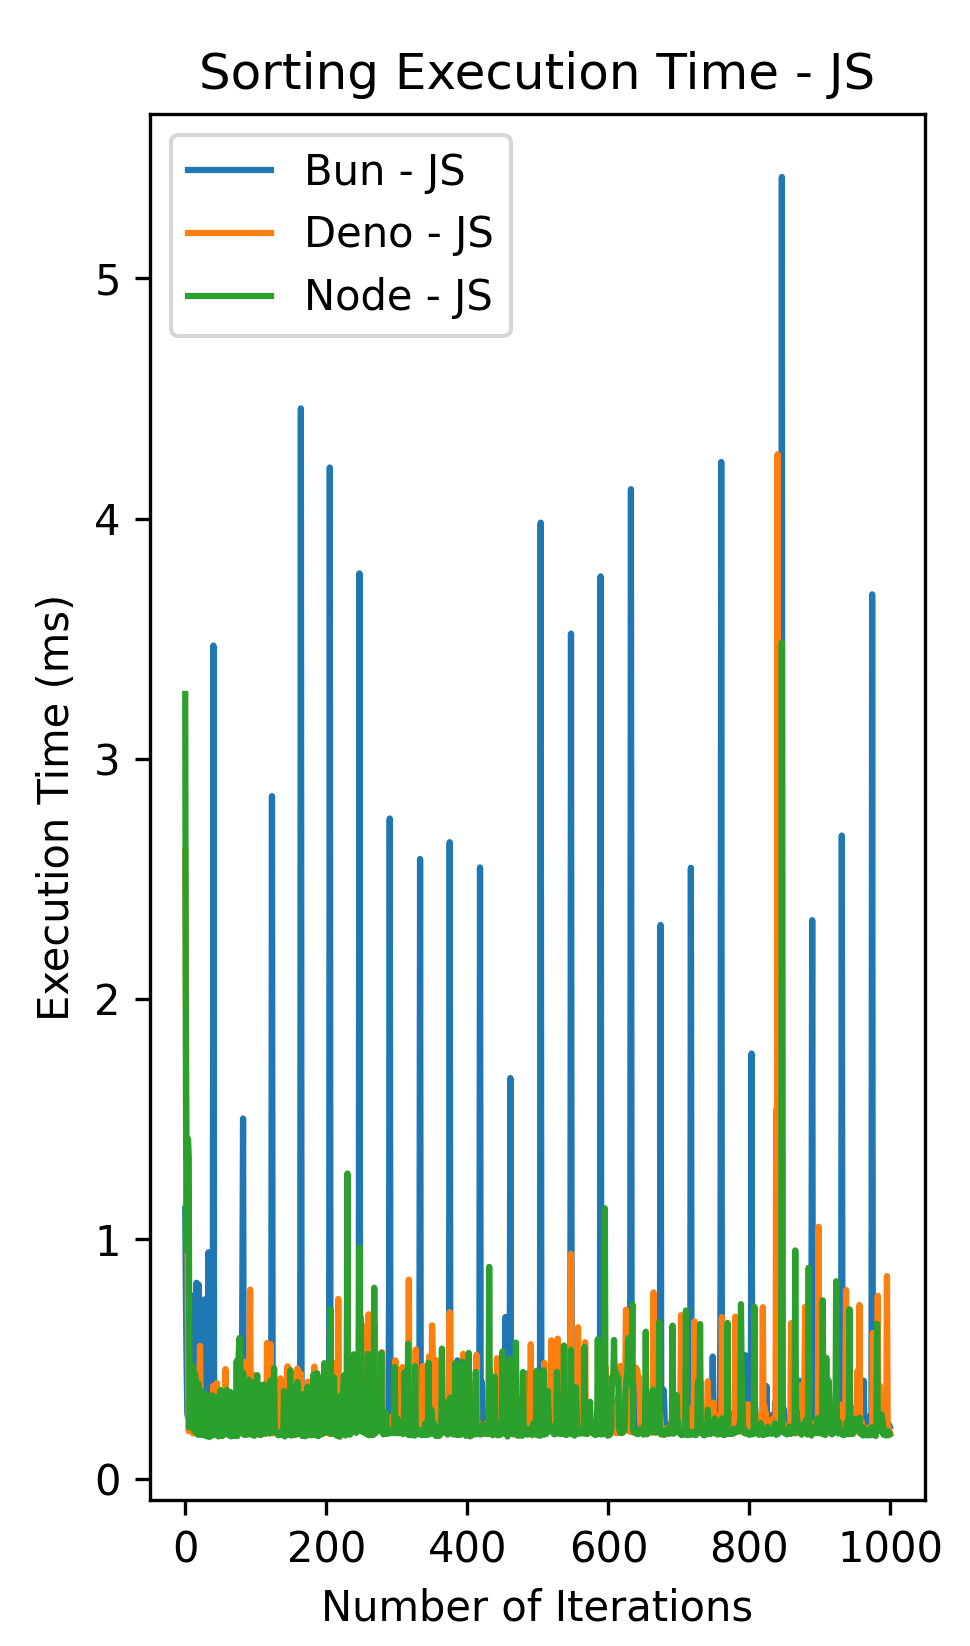
\includegraphics[width=\textwidth]{Figures/sorting/sorting_quick_1000_1000_js_time.png}
    \caption{Czas wykonania testu w milisekundach (ms)}
    \label{fig:quick_sorting_e2_time}
  \end{subfigure}
  \begin{subfigure}[b]{0.42\textwidth}
    \centering
    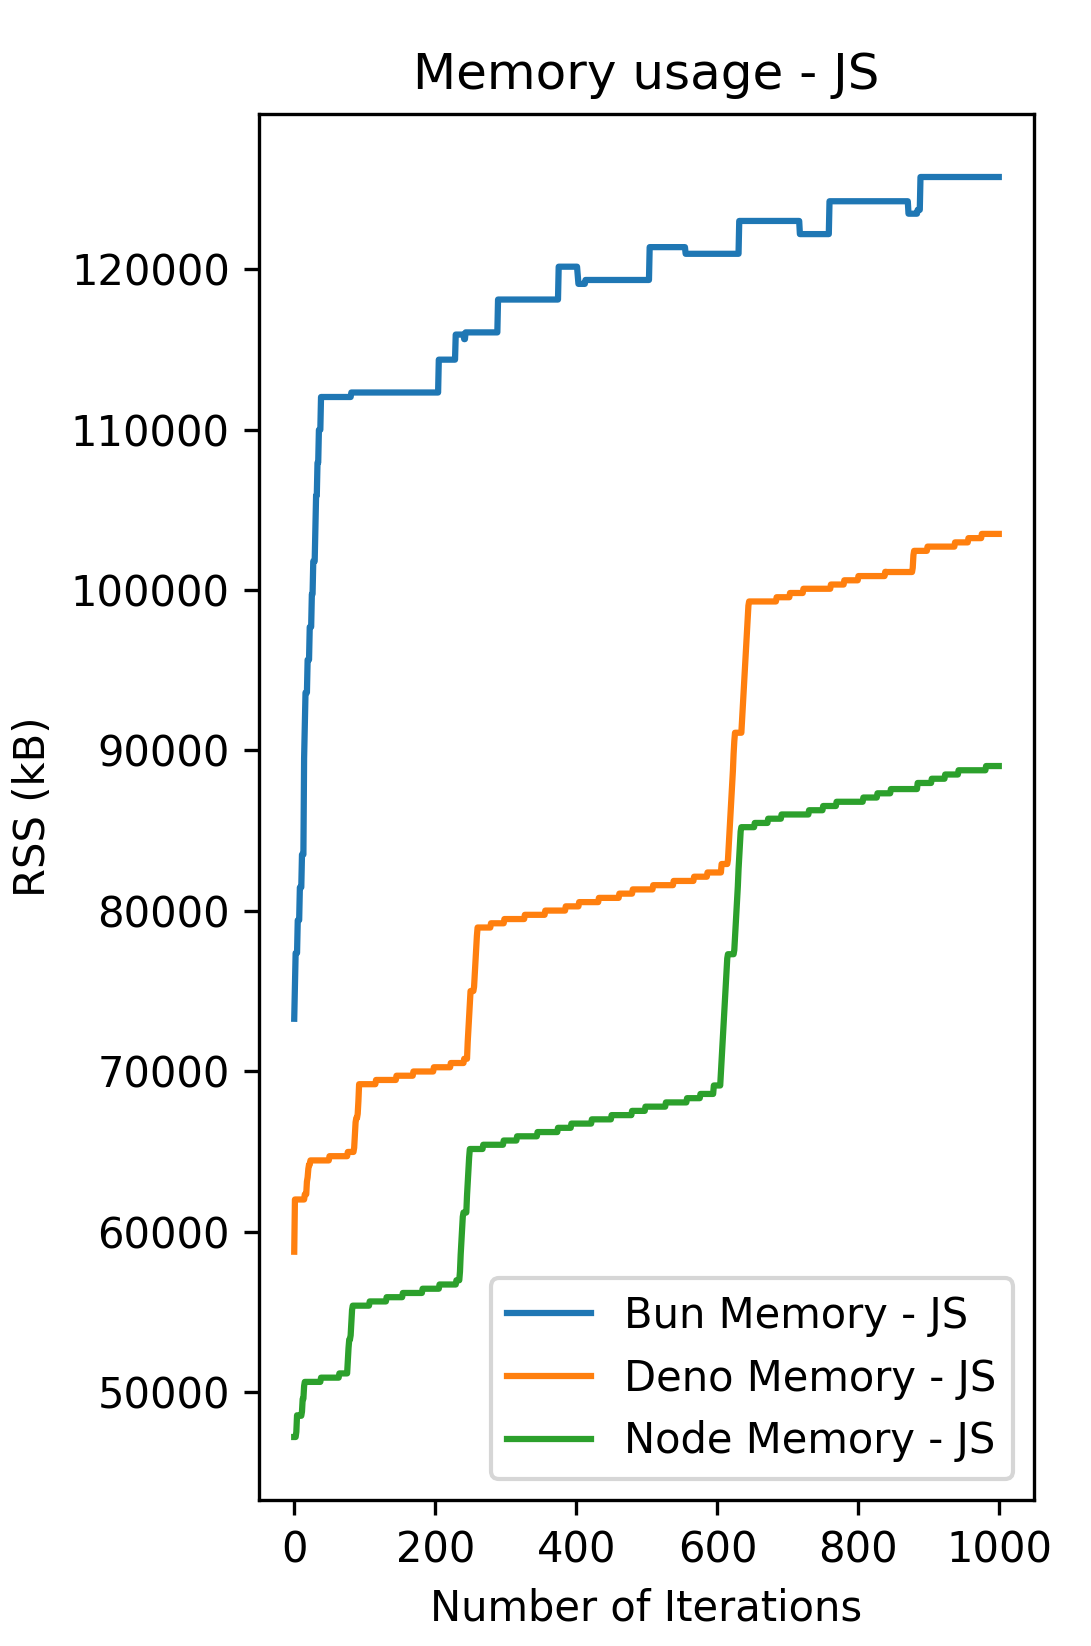
\includegraphics[width=\textwidth]{Figures/sorting/sorting_quick_1000_1000_js_memory.png}
    \caption{Zużycie pamięci operacyjnej w kilobajtach (kB)}
    \label{fig:quick_sorting_e2_memory}
  \end{subfigure}
  \caption{Wyniki eksperymentów dla algorytmu sortowania szybkiego dla 100 iteracji i 1000 elementów - a) czas wykonania jednorazowego testu w milisekundach, b) ilość zajmowanej pamięci w kilobajtach (kB)}
  \label{fig:quick_sorting_e2}
\end{figure}

Na rysunku \ref{fig:quick_sorting_e2_time} możemy zauważyć, że czas wykonania w przypadku pierwszych 10 iteracji jest zwiększony w porównaniu do pozostałych próbek. Natomiast, z wykresu \ref{fig:quick_sorting_e2_memory} możemy zauważyć tendencję wzrostową zużycia pamięci operacyjnej, największym zużyciem pamięci operacyjnej deklaruje środowisko Bun, które w ostatniej iteracji zużywa najwięcej ze wszystkich środowisk uruchomieniowych.

Na rysunku \ref{fig:quick_sorting_e2_ts} przedstawiono wyniki eksperymentów dla algorytmu sortowania szybkiego dla 1000 iteracji i 10000 elementów napisanego w języku TypeScript. Na wykresach przedstawiono czas wykonania jednorazowego testu w milisekundach oraz ilość zajmowanej pamięci w kilobajtach (kB).

\begin{figure}[H]
  \centering
  \begin{subfigure}[b]{0.42\textwidth}
    \centering
    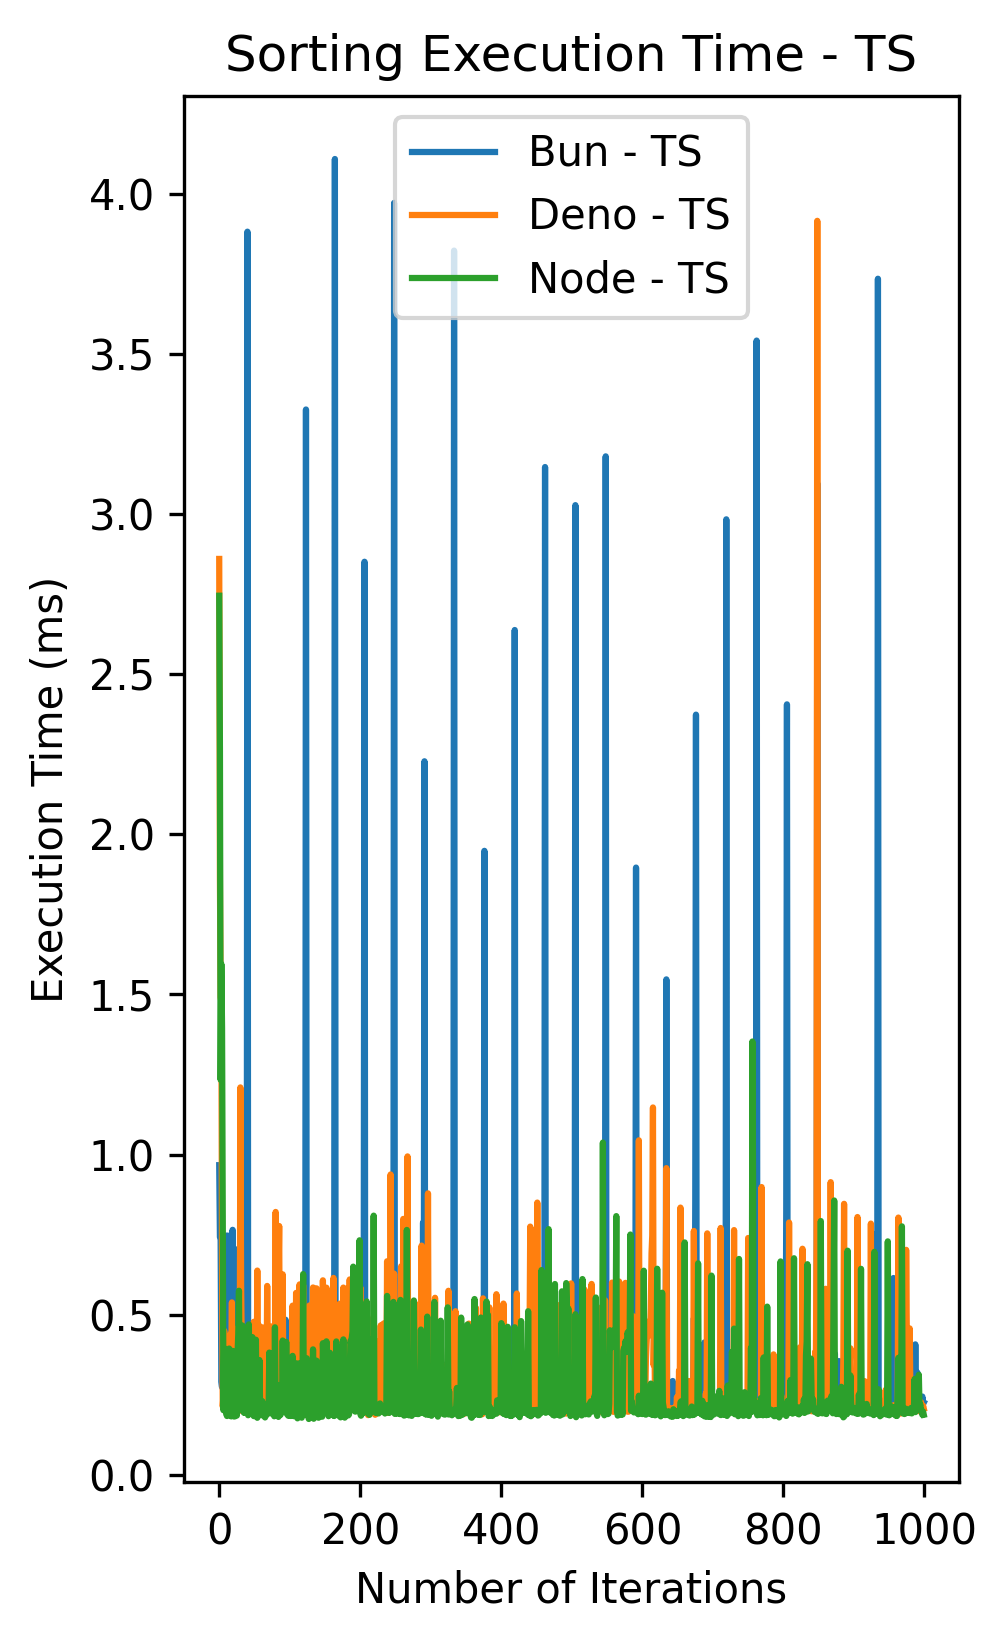
\includegraphics[width=\textwidth]{Figures/sorting/sorting_quick_1000_1000_ts_time.png}
    \caption{Czas wykonania testu w milisekundach (ms)}
    \label{fig:quick_sorting_e2_ts_time}
  \end{subfigure}
  \begin{subfigure}[b]{0.42\textwidth}
    \centering
    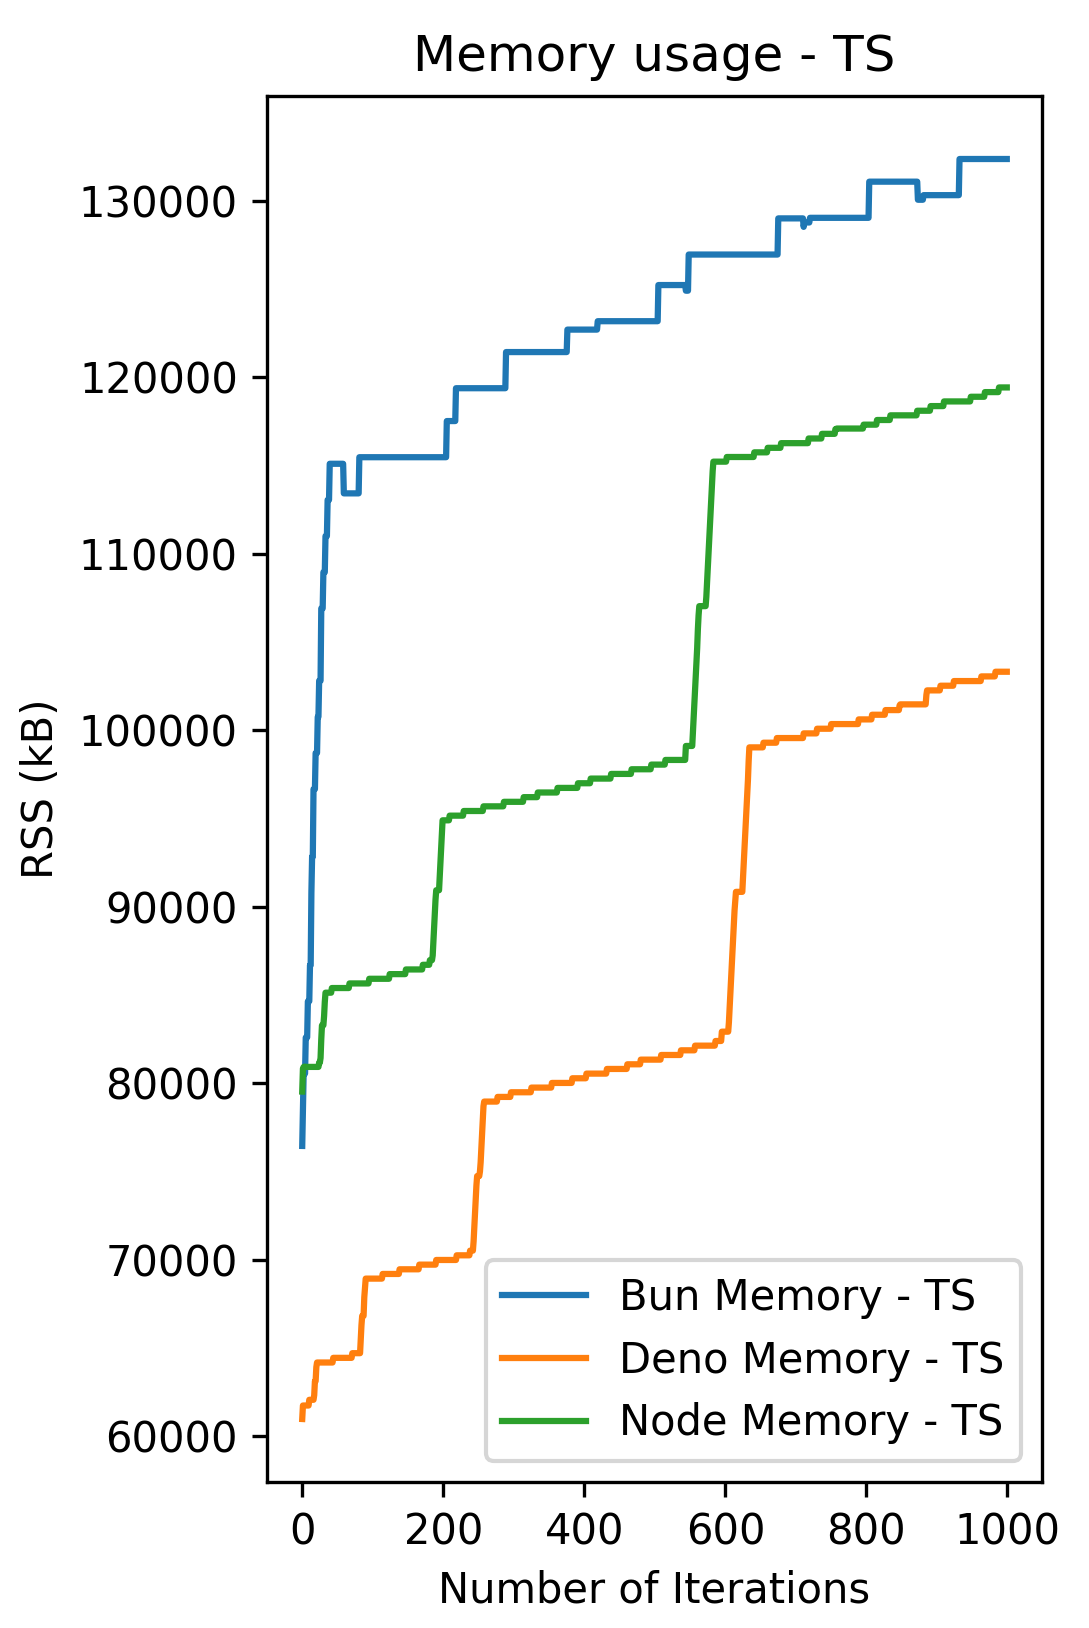
\includegraphics[width=\textwidth]{Figures/sorting/sorting_quick_1000_1000_ts_memory.png}
    \caption{Zużycie pamięci operacyjnej w kilobajtach (kB)}
    \label{fig:quick_sorting_e2_ts_memory}
  \end{subfigure}
  \caption{Wyniki eksperymentów dla algorytmu sortowania szybkiego dla 1000 iteracji i 1000 elementów - a) czas wykonania jednorazowego testu w milisekundach, b) ilość zajmowanej pamięci w kilobajtach (kB)}
  \label{fig:quick_sorting_e2_ts}
\end{figure}

Na rysunku \ref{fig:quick_sorting_e2_ts} przedstawiono czas wykonania testu jak i zużycie pamięci. Na rysunku \ref{fig:quick_sorting_e2_time} zauważono iż, Bun posiadał nierówne czasy wykonania samych eksperymentów, dodatkowo zużycie pamięci operacyjnej w przypadku środowiska Bun było największe ze wszystkich środowisk uruchomieniowych. Najbardziej ustabilizowane czasy wykonania uzyskało środowisko NodeJS, natomiast najmniej pamięci operacyjnej zużyło Deno.

Na rysunku \ref{fig:quick_sorting_e3} przedstawiono wyniki eksperymentów dla algorytmu sortowania szybkiego dla 100 iteracji i 10000 elementów napisanego w języku JavaScript. Na wykresach przedstawiono czas wykonania jednorazowego testu w milisekundach oraz ilość zajmowanej pamięci w kilobajtach (kB).

\begin{figure}[H]
  \centering
  \begin{subfigure}[b]{0.42\textwidth}
    \centering
    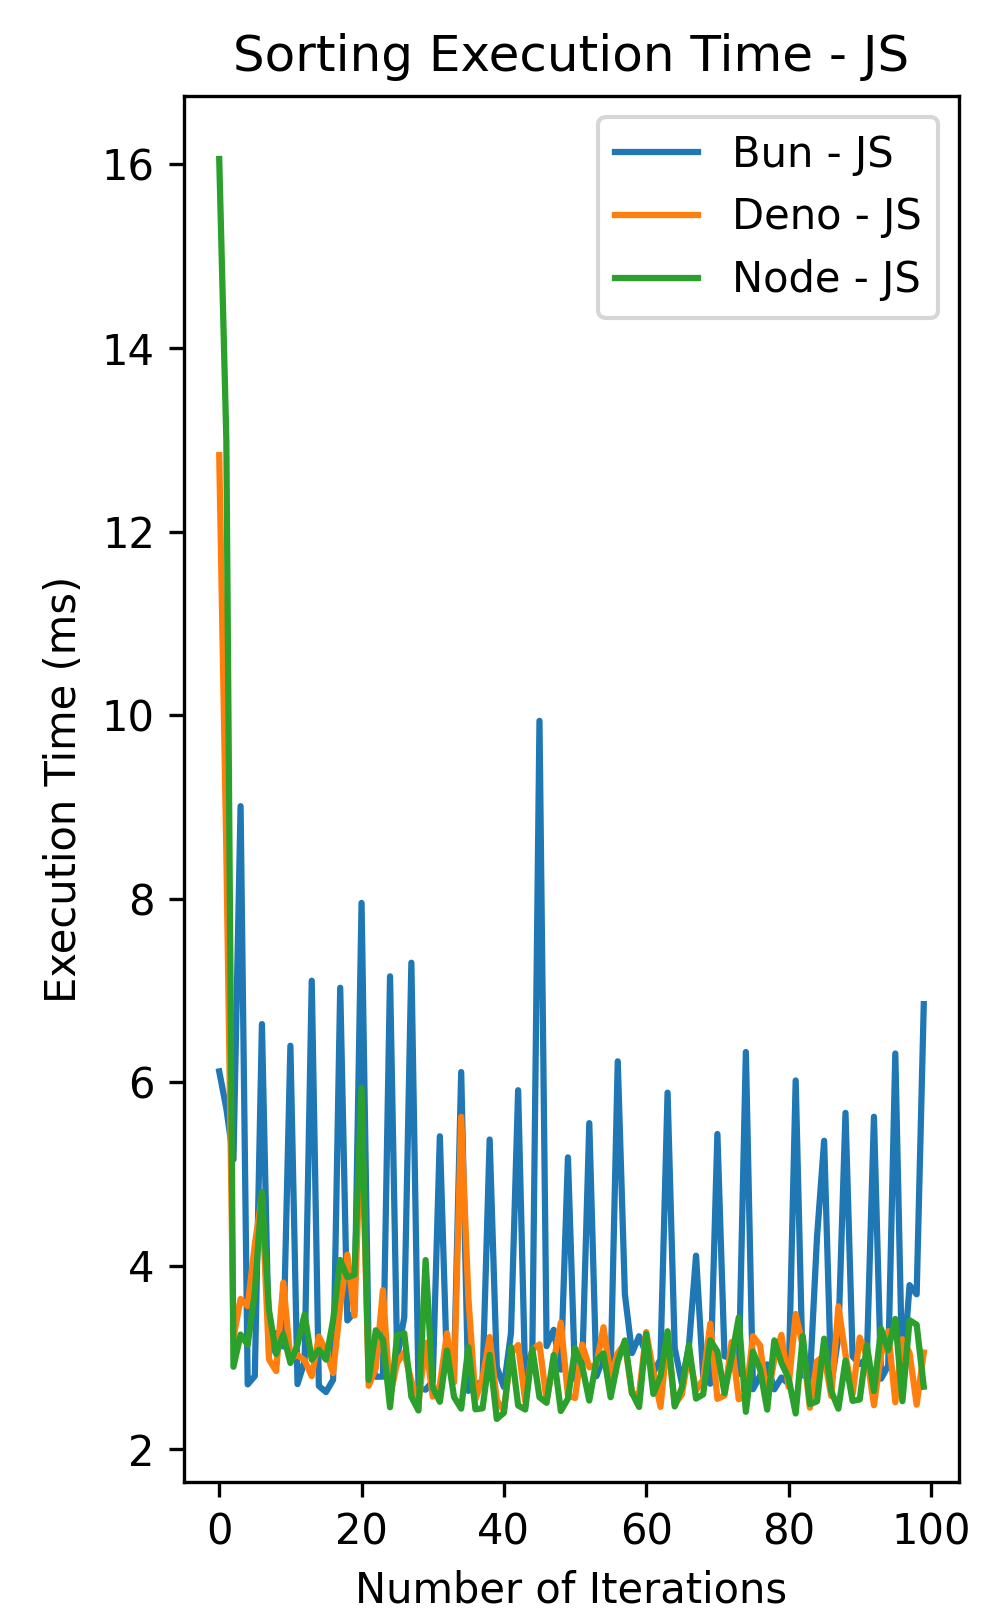
\includegraphics[width=\textwidth]{Figures/sorting/sorting_quick_100_10000_js_time.png}
    \caption{Czas wykonania testu w milisekundach (ms)}
    \label{fig:quick_sorting_e3_time}
  \end{subfigure}
  \begin{subfigure}[b]{0.42\textwidth}
    \centering
    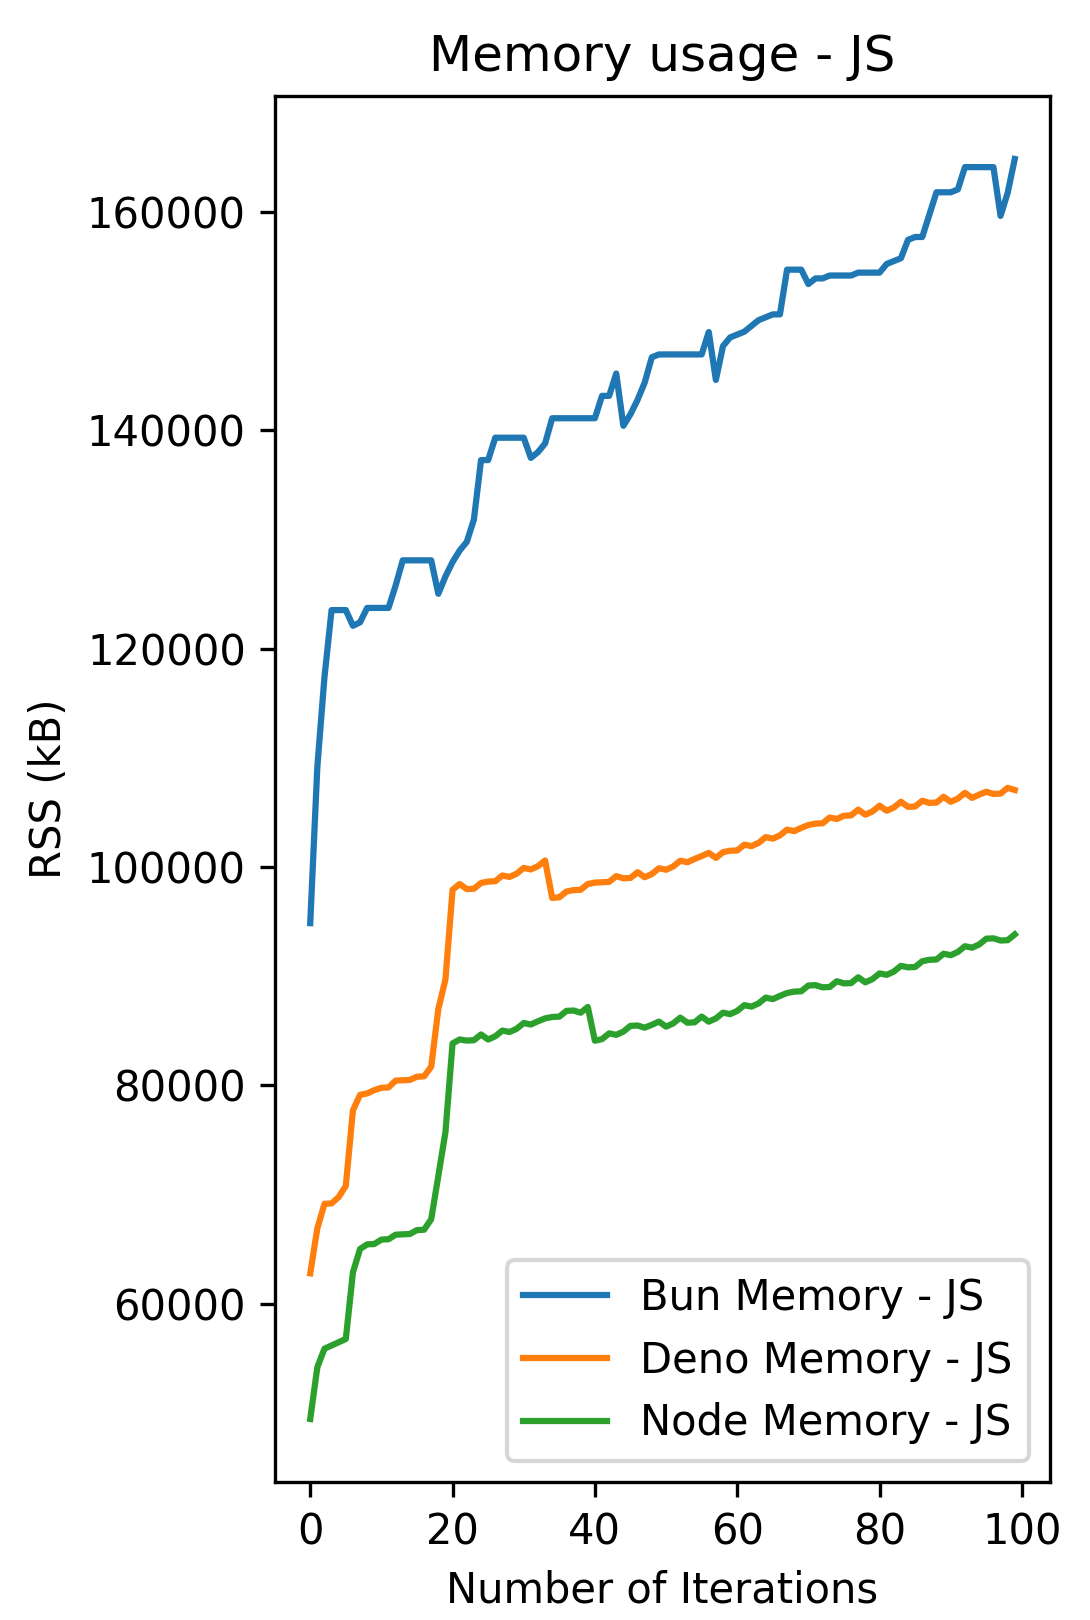
\includegraphics[width=\textwidth]{Figures/sorting/sorting_quick_100_10000_js_memory.png}
    \caption{Zużycie pamięci operacyjnej w kilobajtach (kB)}
    \label{fig:quick_sorting_e3_memory}
  \end{subfigure}
  \caption{Wyniki eksperymentów dla algorytmu sortowania szybkiego dla 100 iteracji i 10000 elementów - a) czas wykonania jednorazowego testu w milisekundach, b) ilość zajmowanej pamięci w kilobajtach (kB)}
  \label{fig:quick_sorting_e3}
\end{figure}

Na rysunku \ref{fig:quick_sorting_e3_time} zauważono, że NodeJS posiadał najdłuższe czasy wykonywania sortowania w pierwszych iteracjach, natomiast największe rozbieżności w czasach wykonania posiadało środowisko Bun. Z wykresu \ref{fig:quick_sorting_e3_memory} zauważono, że środowisko Bun zużywało najwięcej pamięci operacyjnej, natomiast środowisko Deno zużywało najmniej pamięci operacyjnej.

Na rysunku \ref{fig:quick_sorting_e3_ts} przedstawiono wyniki eksperymentów dla algorytmu sortowania szybkiego dla 1000 iteracji i 1000 elementów napisanego w języku TypeScript. Na wykresach przedstawiono czas wykonania jednorazowego testu w milisekundach oraz ilość zajmowanej pamięci w kilobajtach (kB).

\begin{figure}[H]
  \centering
  \begin{subfigure}[b]{0.42\textwidth}
    \centering
    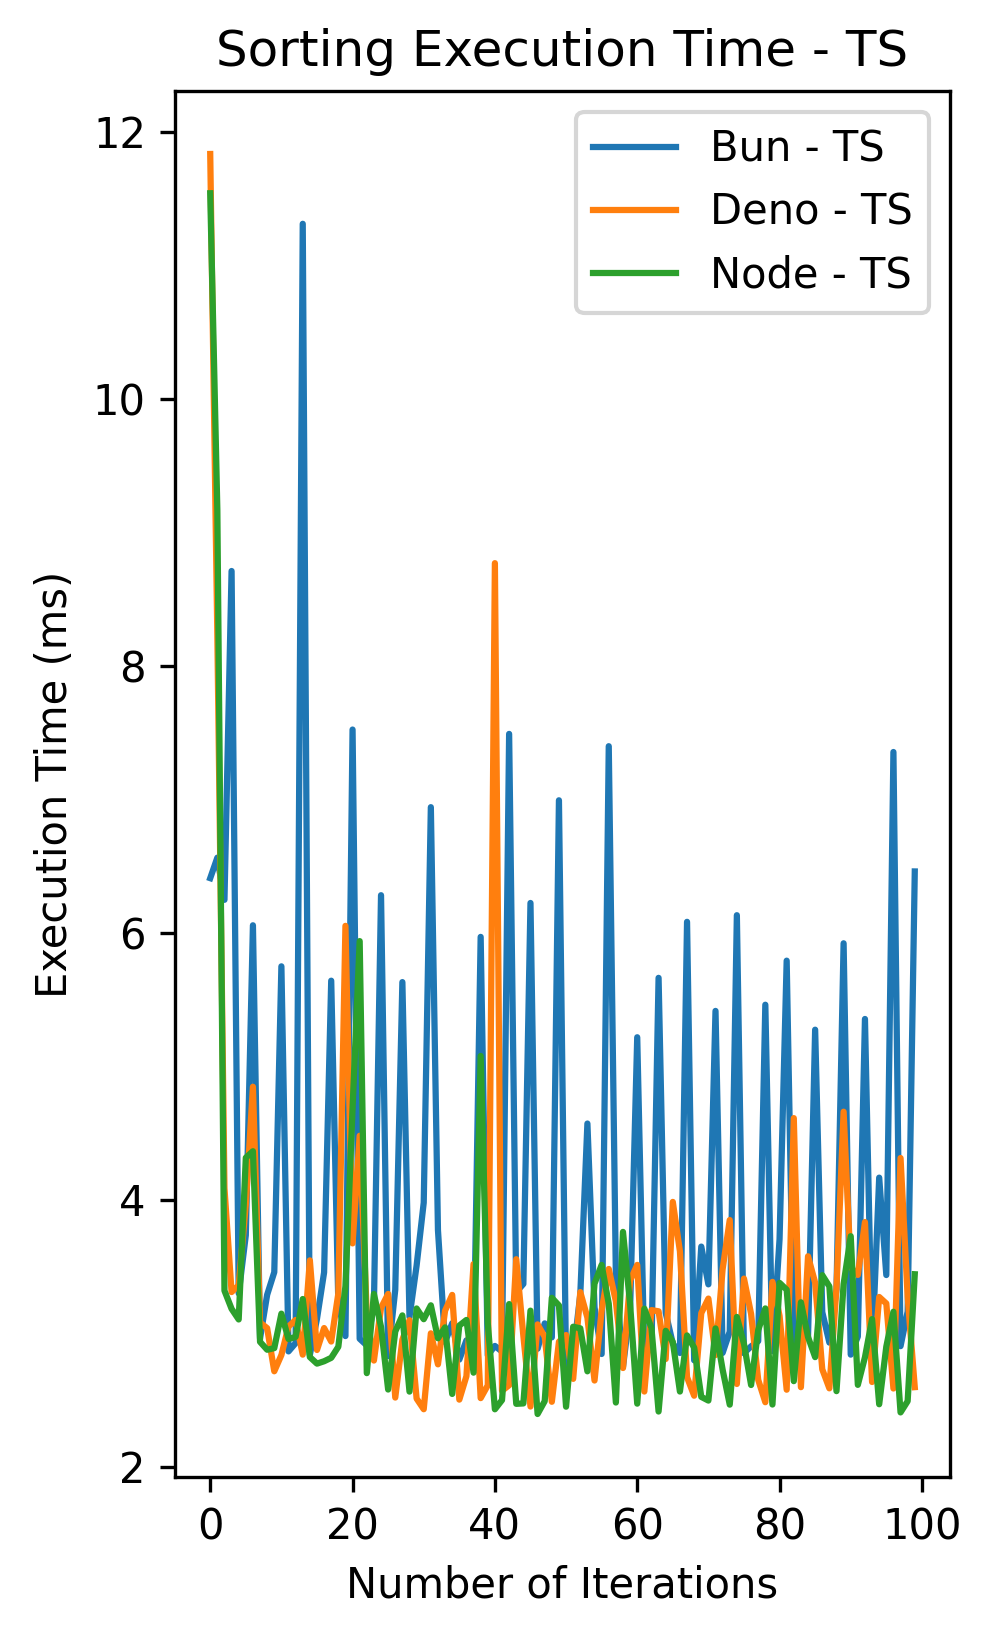
\includegraphics[width=\textwidth]{Figures/sorting/sorting_quick_100_10000_ts_time.png}
    \caption{Czas wykonania testu w milisekundach (ms)}
    \label{fig:quick_sorting_e3_ts_time}
  \end{subfigure}
  \begin{subfigure}[b]{0.42\textwidth}
    \centering
    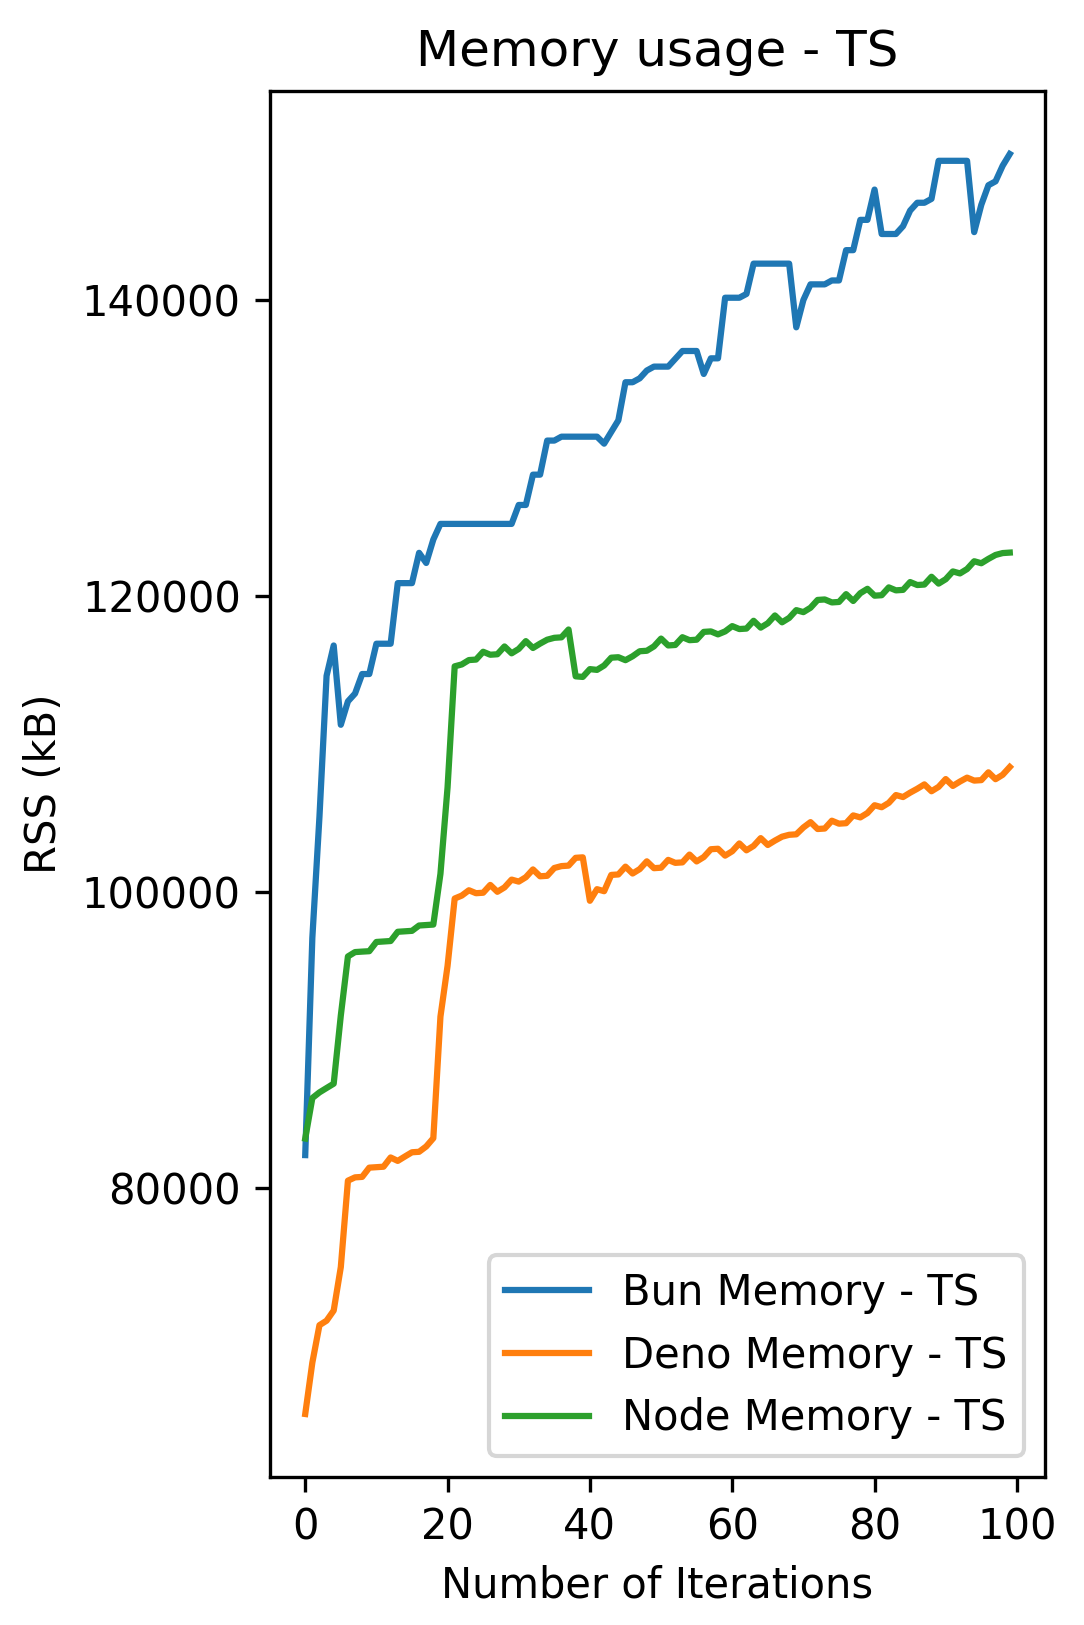
\includegraphics[width=\textwidth]{Figures/sorting/sorting_quick_100_10000_ts_memory.png}
    \caption{Zużycie pamięci operacyjnej w kilobajtach (kB)}
    \label{fig:quick_sorting_e3_ts_memory}
  \end{subfigure}
  \caption{Wyniki eksperymentów dla algorytmu sortowania szybkiego dla 100 iteracji i 10000 elementów - a) czas wykonania jednorazowego testu w milisekundach, b) ilość zajmowanej pamięci w kilobajtach (kB)}
  \label{fig:quick_sorting_e3_ts}
\end{figure}

Na rysunku \ref{fig:quick_sorting_e3_ts_time} zauważono, że Deno posiadał najdłuższe czasy wykonywania sortowania w pierwszych iteracjach, natomiast największe rozbieżności w czasach wykonania posiadało środowisko Bun. Z wykresu \ref{fig:quick_sorting_e3_ts_memory} zauważono, że środowisko Bun zużywało najwięcej pamięci operacyjnej, natomiast środowisko Deno zużywało najmniej pamięci operacyjnej.

Na rysunku \ref{fig:quick_sorting_e4} przedstawiono wyniki eksperymentów dla algorytmu sortowania szybkiego dla 1000 iteracji i 10000 elementów napisanego w języku JavaScript. Na wykresach przedstawiono czas wykonania jednorazowego testu w milisekundach oraz ilość zajmowanej pamięci w kilobajtach (kB).

\begin{figure}[H]
  \centering
  \begin{subfigure}[b]{0.42\textwidth}
    \centering
    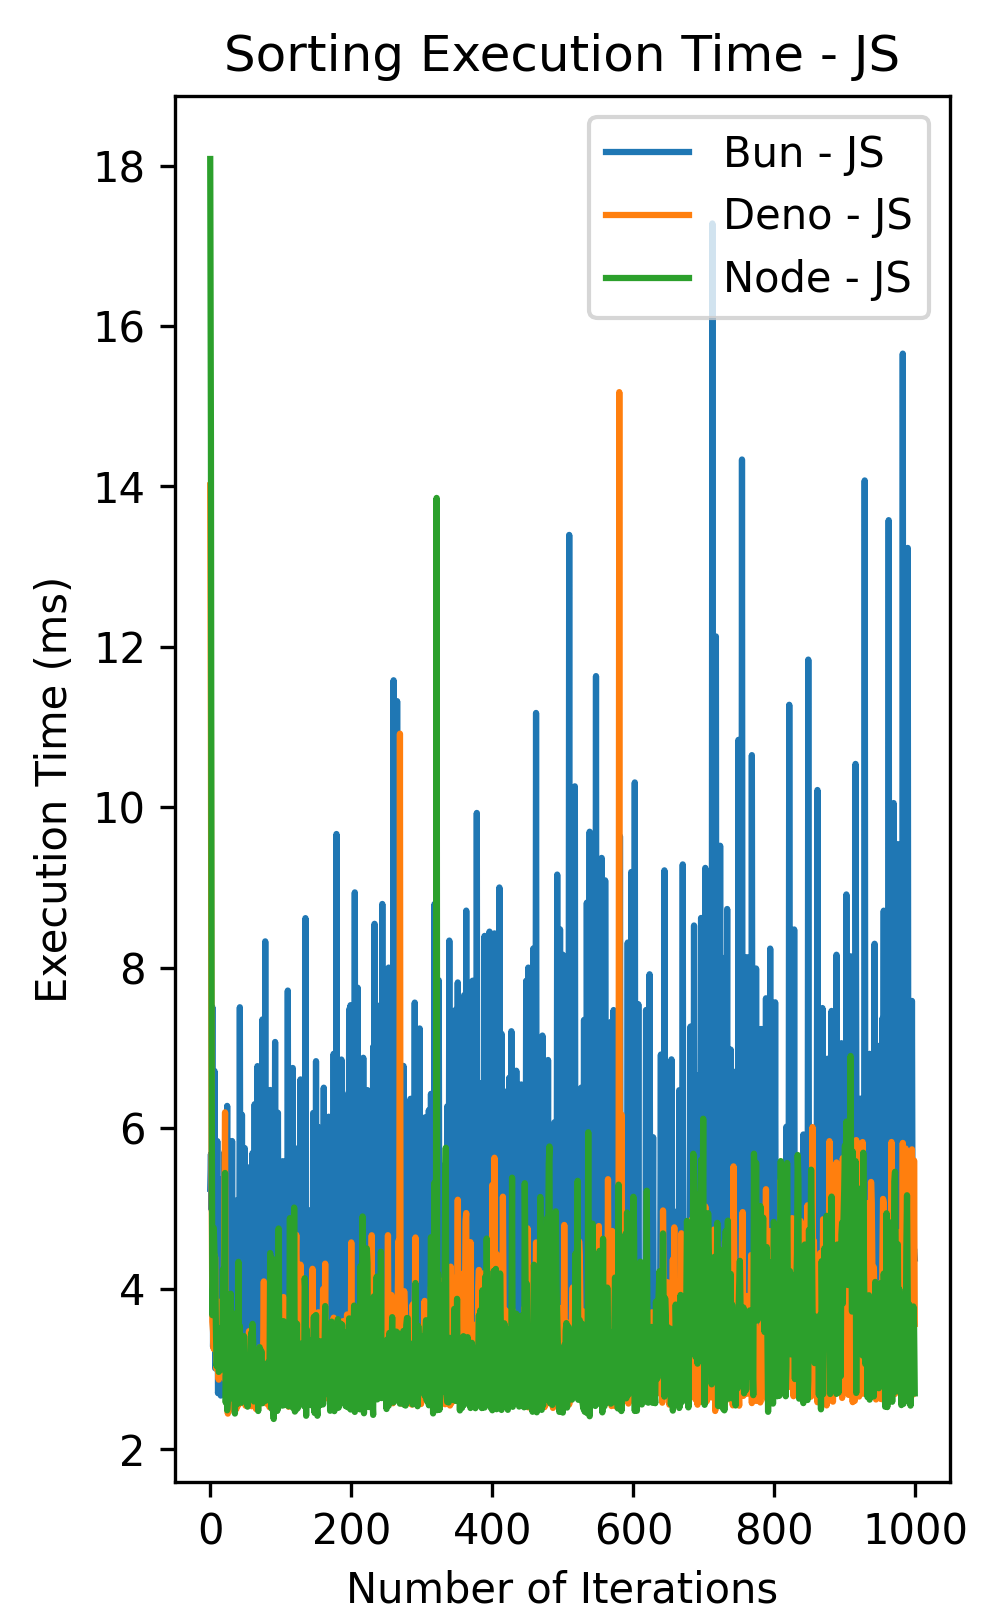
\includegraphics[width=\textwidth]{Figures/sorting/sorting_quick_1000_10000_js_time.png}
    \caption{Czas wykonania testu w milisekundach (ms)}
    \label{fig:quick_sorting_e4_time}
  \end{subfigure}
  \begin{subfigure}[b]{0.42\textwidth}
    \centering
    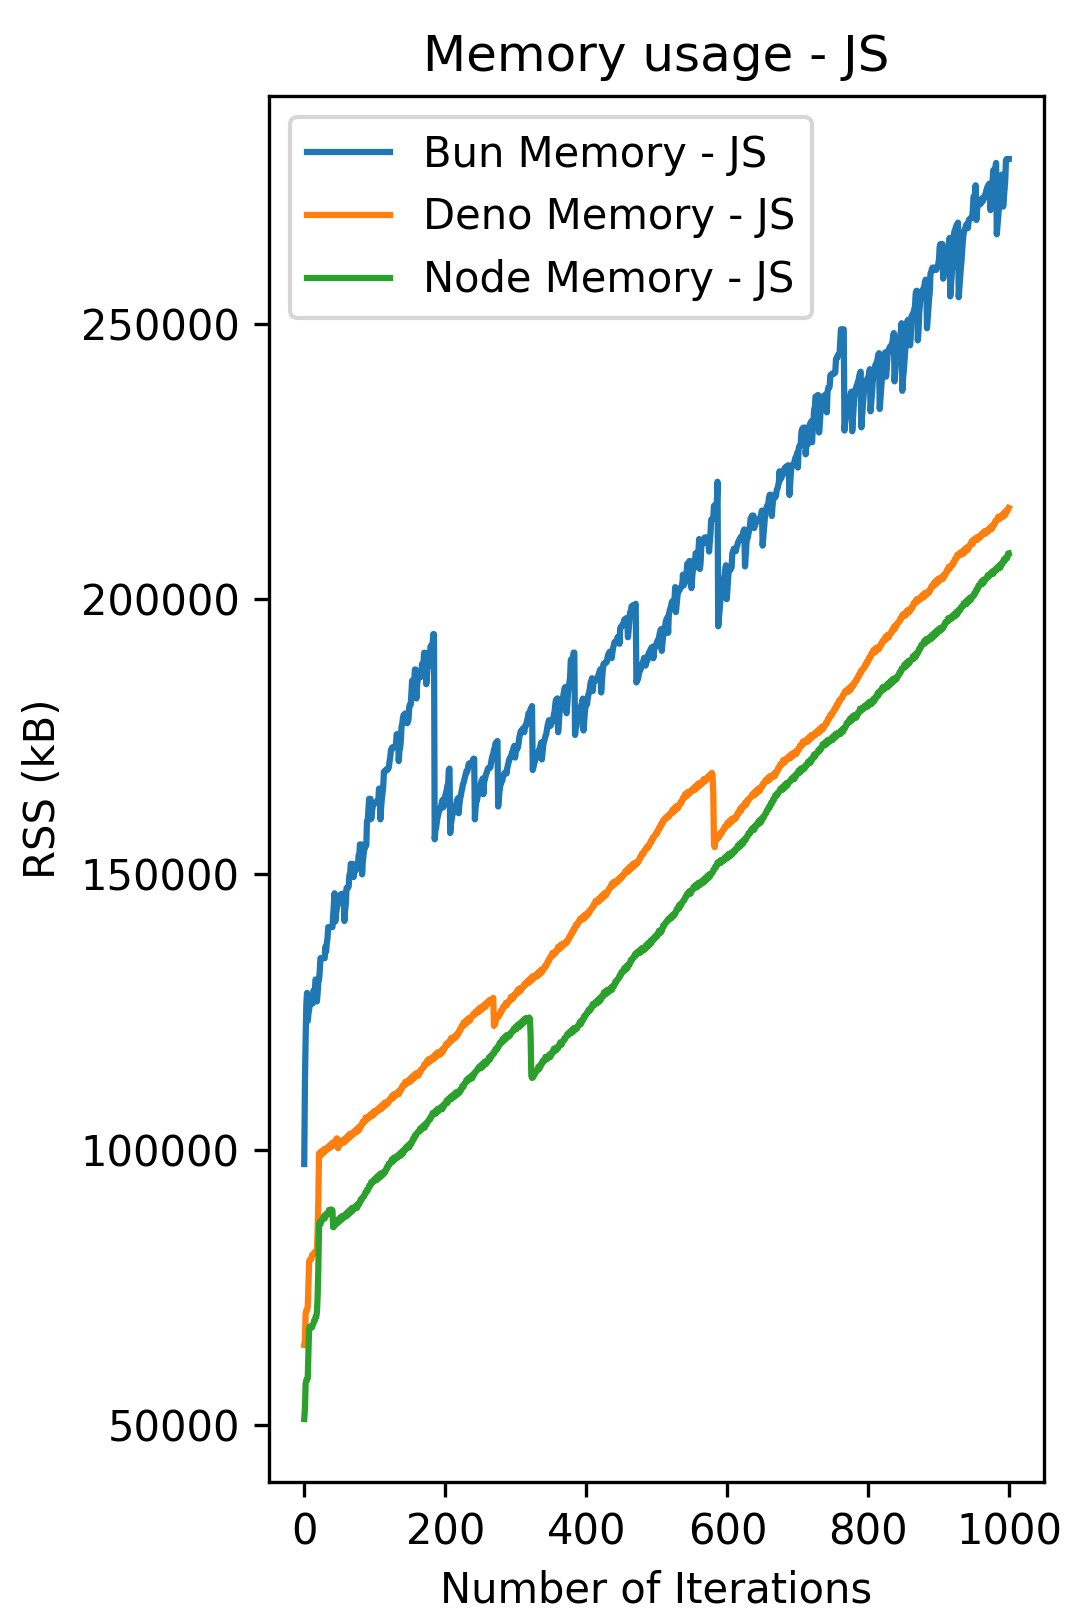
\includegraphics[width=\textwidth]{Figures/sorting/sorting_quick_1000_10000_js_memory.png}
    \caption{Zużycie pamięci operacyjnej w kilobajtach (kB)}
    \label{fig:quick_sorting_e4_memory}
  \end{subfigure}
  \caption{Wyniki eksperymentów dla algorytmu sortowania szybkiego dla 1000 iteracji i 10000 elementów - a) czas wykonania jednorazowego testu w milisekundach, b) ilość zajmowanej pamięci w kilobajtach (kB)}
  \label{fig:quick_sorting_e4}
\end{figure}

Na rysunku \ref{fig:quick_sorting_e4_time} zauważono, że NodeJS posiadał najdłuższe czasy wykonywania sortowania w pierwszych iteracjach, natomiast największe rozbieżności w czasach wykonania posiadało środowisko Bun. W przypadku zwiększonej liczby elementów, zauważono na wykresie \ref{fig:quick_sorting_e4_memory} podobną ilość pamięci zajmują środowiska NodeJS oraz Deno.

Na rysunku \ref{fig:quick_sorting_e4_ts} przedstawiono wyniki eksperymentów dla algorytmu sortowania szybkiego dla 100 iteracji i 10000 elementów napisanego w języku TypeScript. Na wykresach przedstawiono czas wykonania jednorazowego testu w milisekundach oraz ilość zajmowanej pamięci w kilobajtach (kB).

\begin{figure}[H]
  \centering
  \begin{subfigure}[b]{0.42\textwidth}
    \centering
    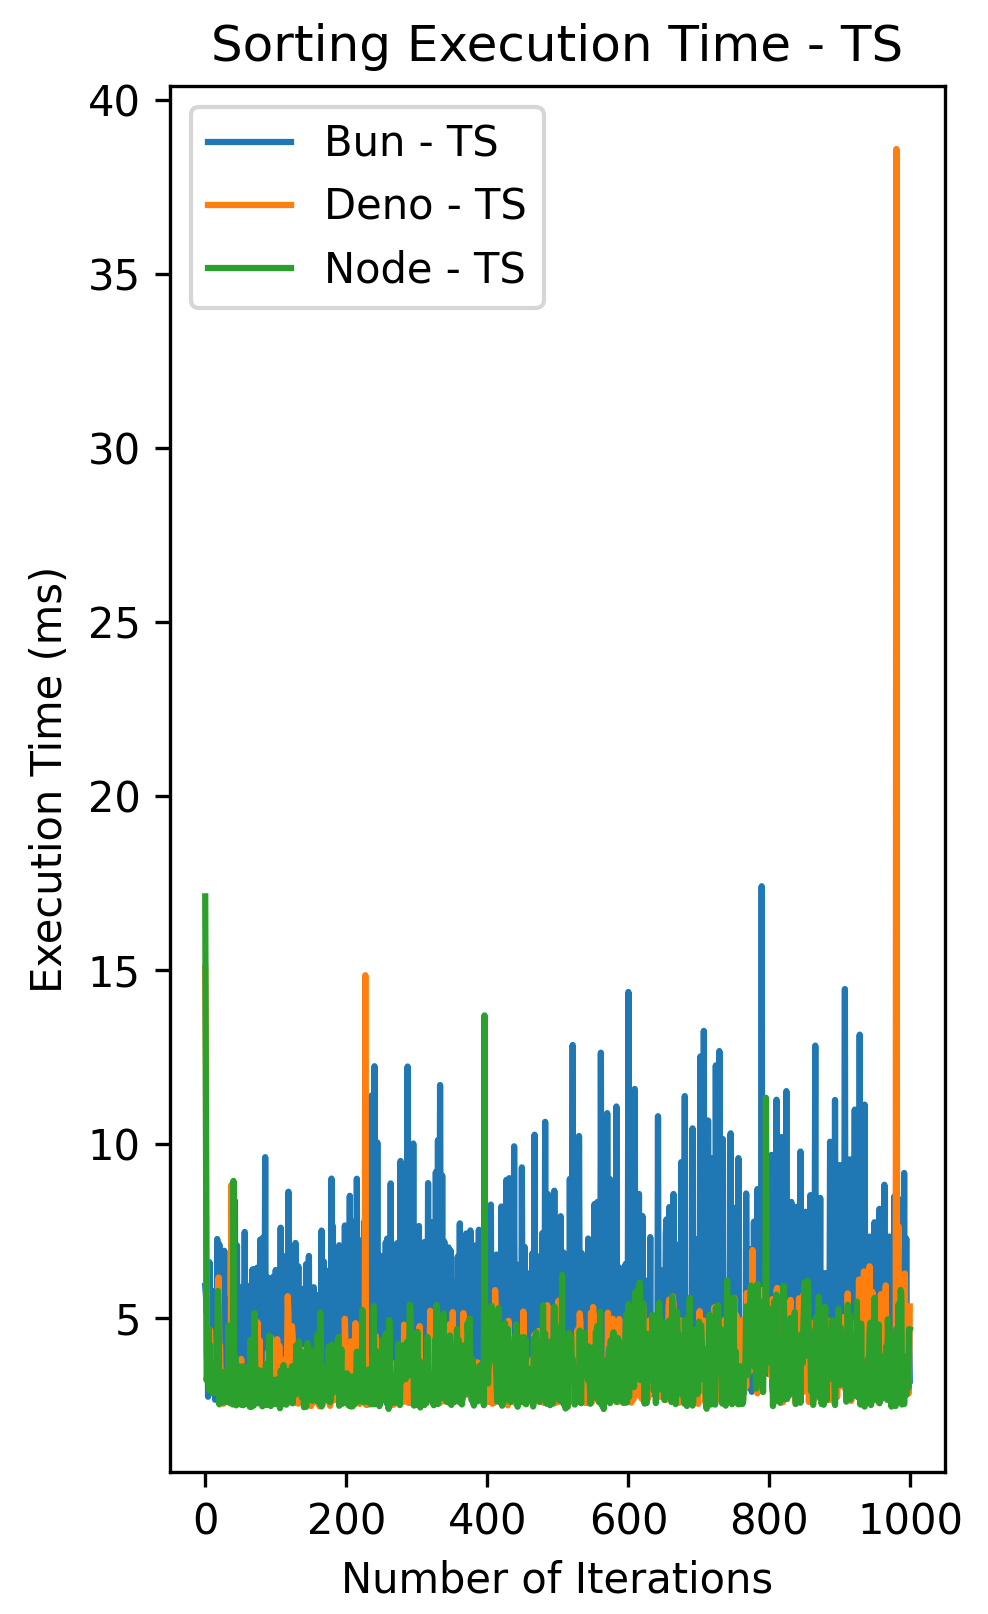
\includegraphics[width=\textwidth]{Figures/sorting/sorting_quick_1000_10000_ts_time.png}
    \caption{Czas wykonania testu w milisekundach (ms)}
    \label{fig:quick_sorting_e4_ts_time}
  \end{subfigure}
  \begin{subfigure}[b]{0.42\textwidth}
    \centering
    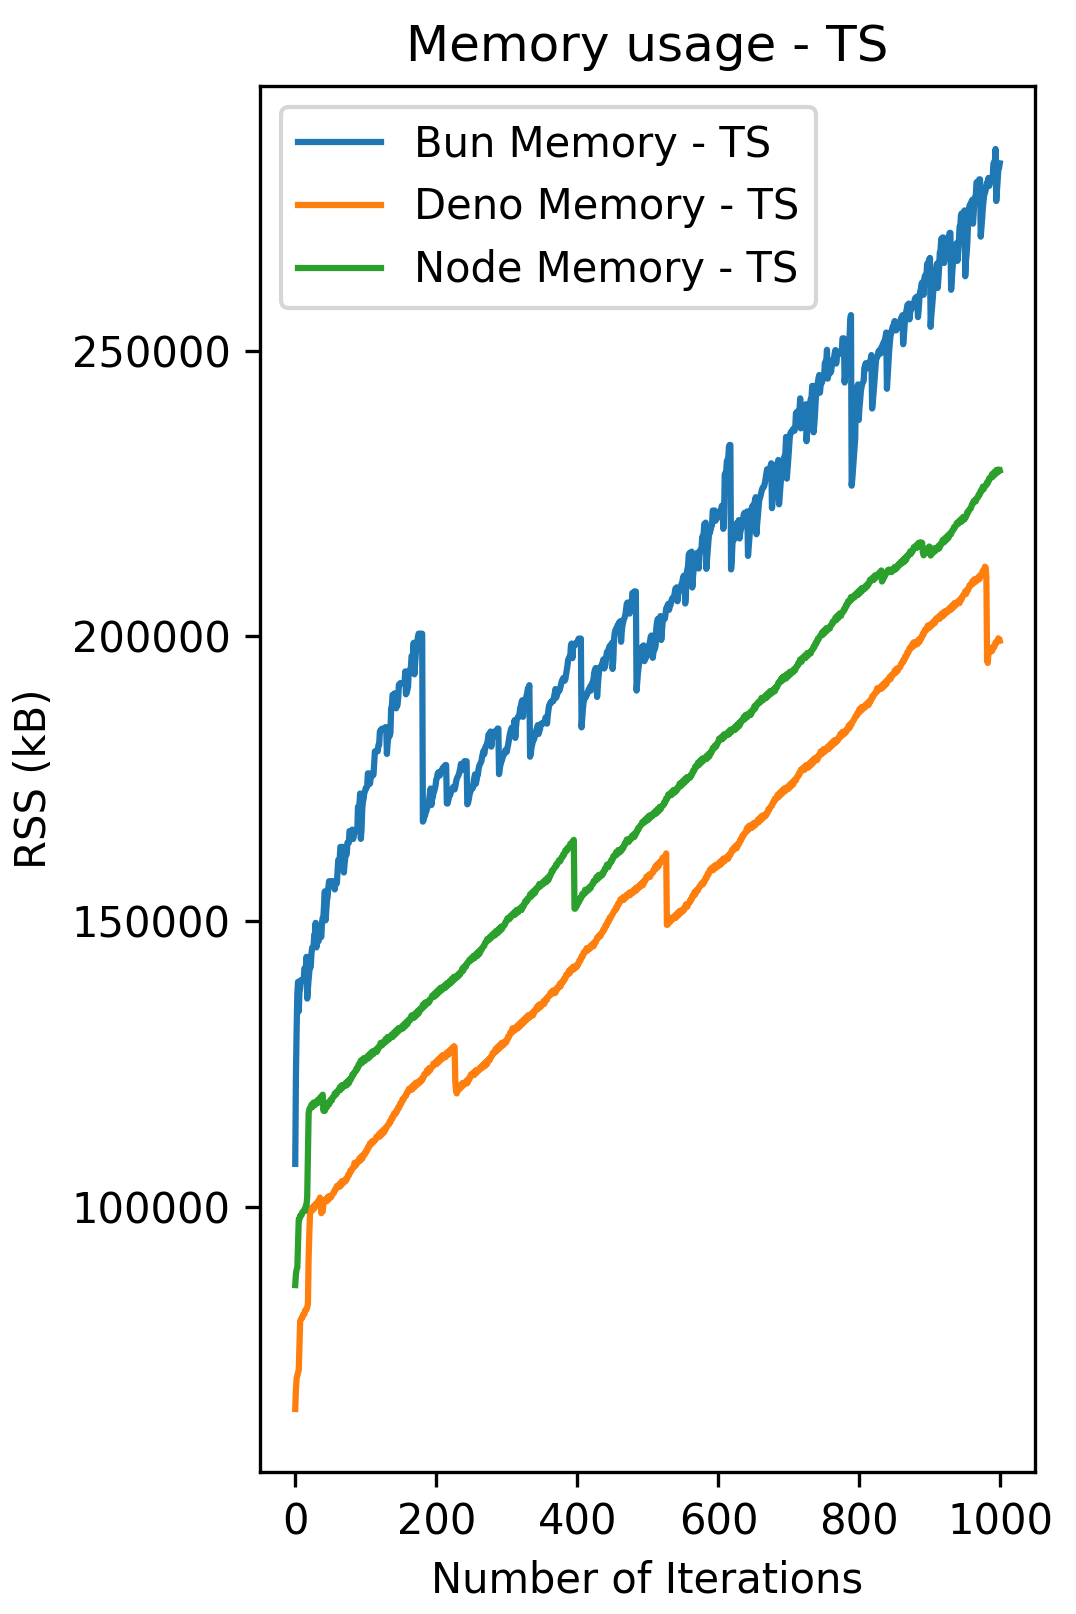
\includegraphics[width=\textwidth]{Figures/sorting/sorting_quick_1000_10000_ts_memory.png}
    \caption{Zużycie pamięci operacyjnej w kilobajtach (kB)}
    \label{fig:quick_sorting_e4_ts_memory}
  \end{subfigure}
  \caption{Wyniki eksperymentów dla algorytmu sortowania szybkiego dla 1000 iteracji i 10000 elementów - a) czas wykonania jednorazowego testu w milisekundach, b) ilość zajmowanej pamięci w kilobajtach (kB)}
  \label{fig:quick_sorting_e4_ts}
\end{figure}

Na rysunku \ref{fig:quick_sorting_e4_ts_time} zauważono, że NodeJS posiadał najdłuższe czasy wykonywania sortowania w pierwszych iteracjach, natomiast największe rozbieżności w czasach wykonania posiadało środowisko Bun. Na rysunku \ref{fig:quick_sorting_e4_ts_memory} podczas jednej z ostatnich iteracji możemy zauważyć zwolnienie pamięci przez środowisko Deno, co może być spowodowane działaniem mechanizmu Garbage Collector. Natomiast największym zużyciem pamięci operacyjnej deklaruje środowisko Bun, które w ostatniej iteracji zużywa najwięcej ze wszystkich środowisk uruchomieniowych.

\subsubsection{Wyniki - sortowanie pozycyjne}
Na rysunku \ref{fig:radix_sorting_e1} przedstawiono wyniki eksperymentów dla algorytmu sortowania pozycyjnego dla 100 iteracji i 1000 elementów napisanego w języku JavaScript. Na wykresach przedstawiono czas wykonania jednorazowego testu w milisekundach oraz ilość zajmowanej pamięci w kilobajtach (kB).

\begin{figure}[H]
  \centering
  \begin{subfigure}[b]{0.42\textwidth}
    \centering
    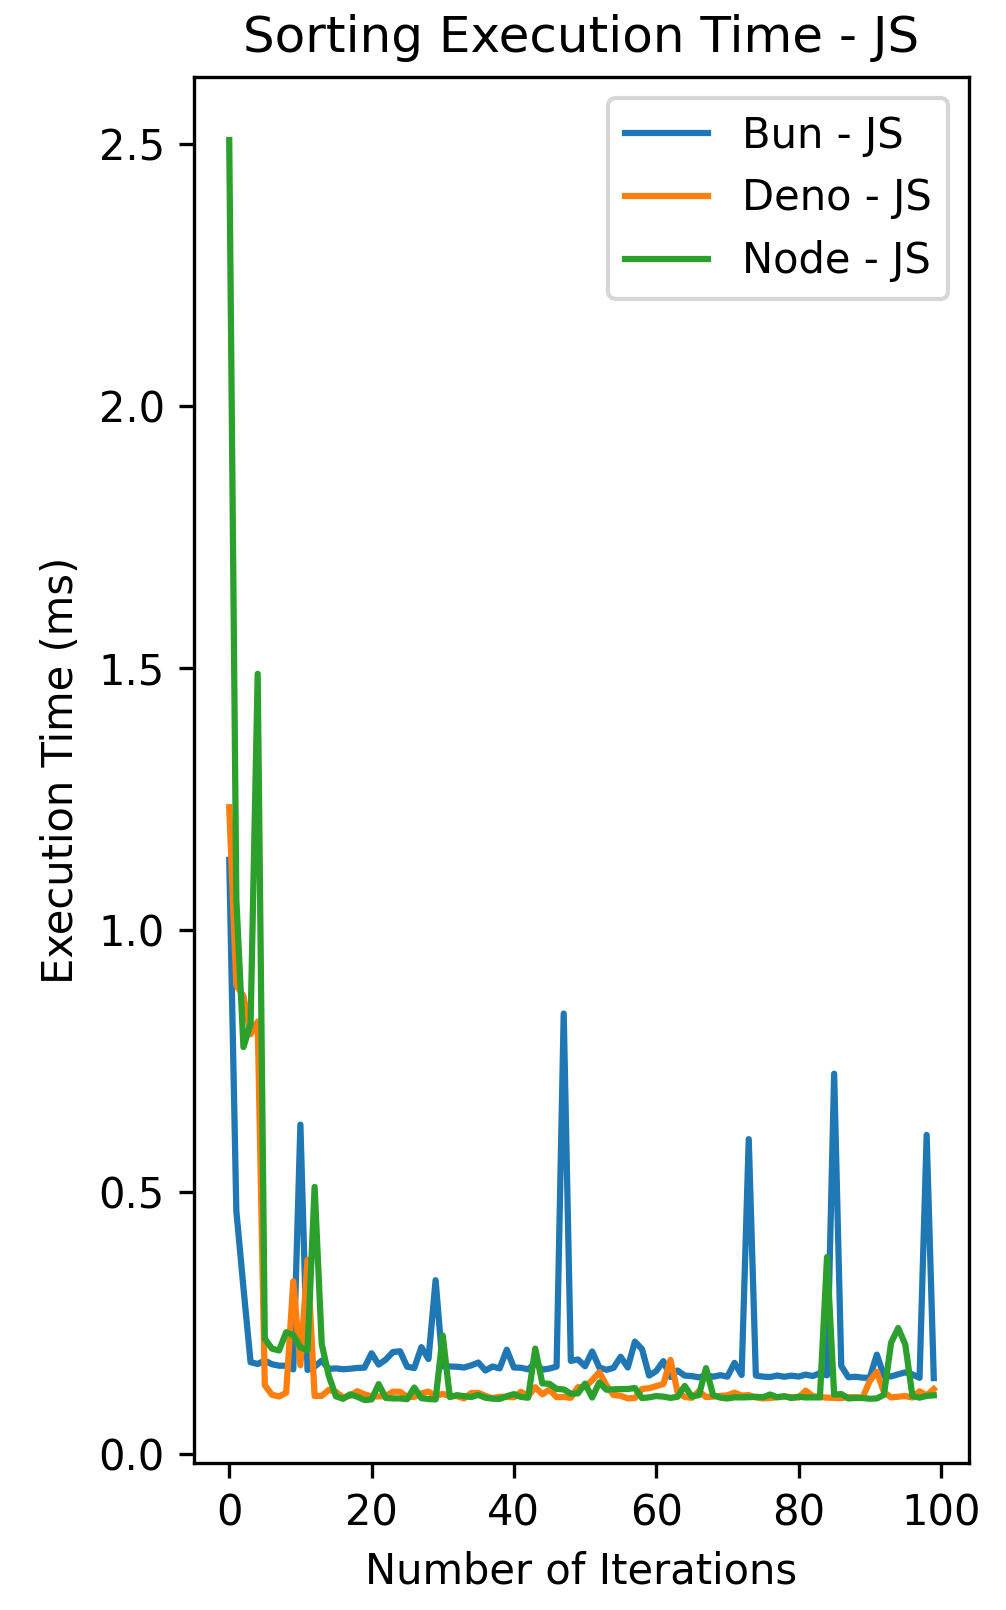
\includegraphics[width=\textwidth]{Figures/sorting/sorting_radix_100_1000_js_time.png}
    \caption{Czas wykonania testu w milisekundach (ms)}
    \label{fig:radix_sorting_e1_time}
  \end{subfigure}
  \begin{subfigure}[b]{0.42\textwidth}
    \centering
    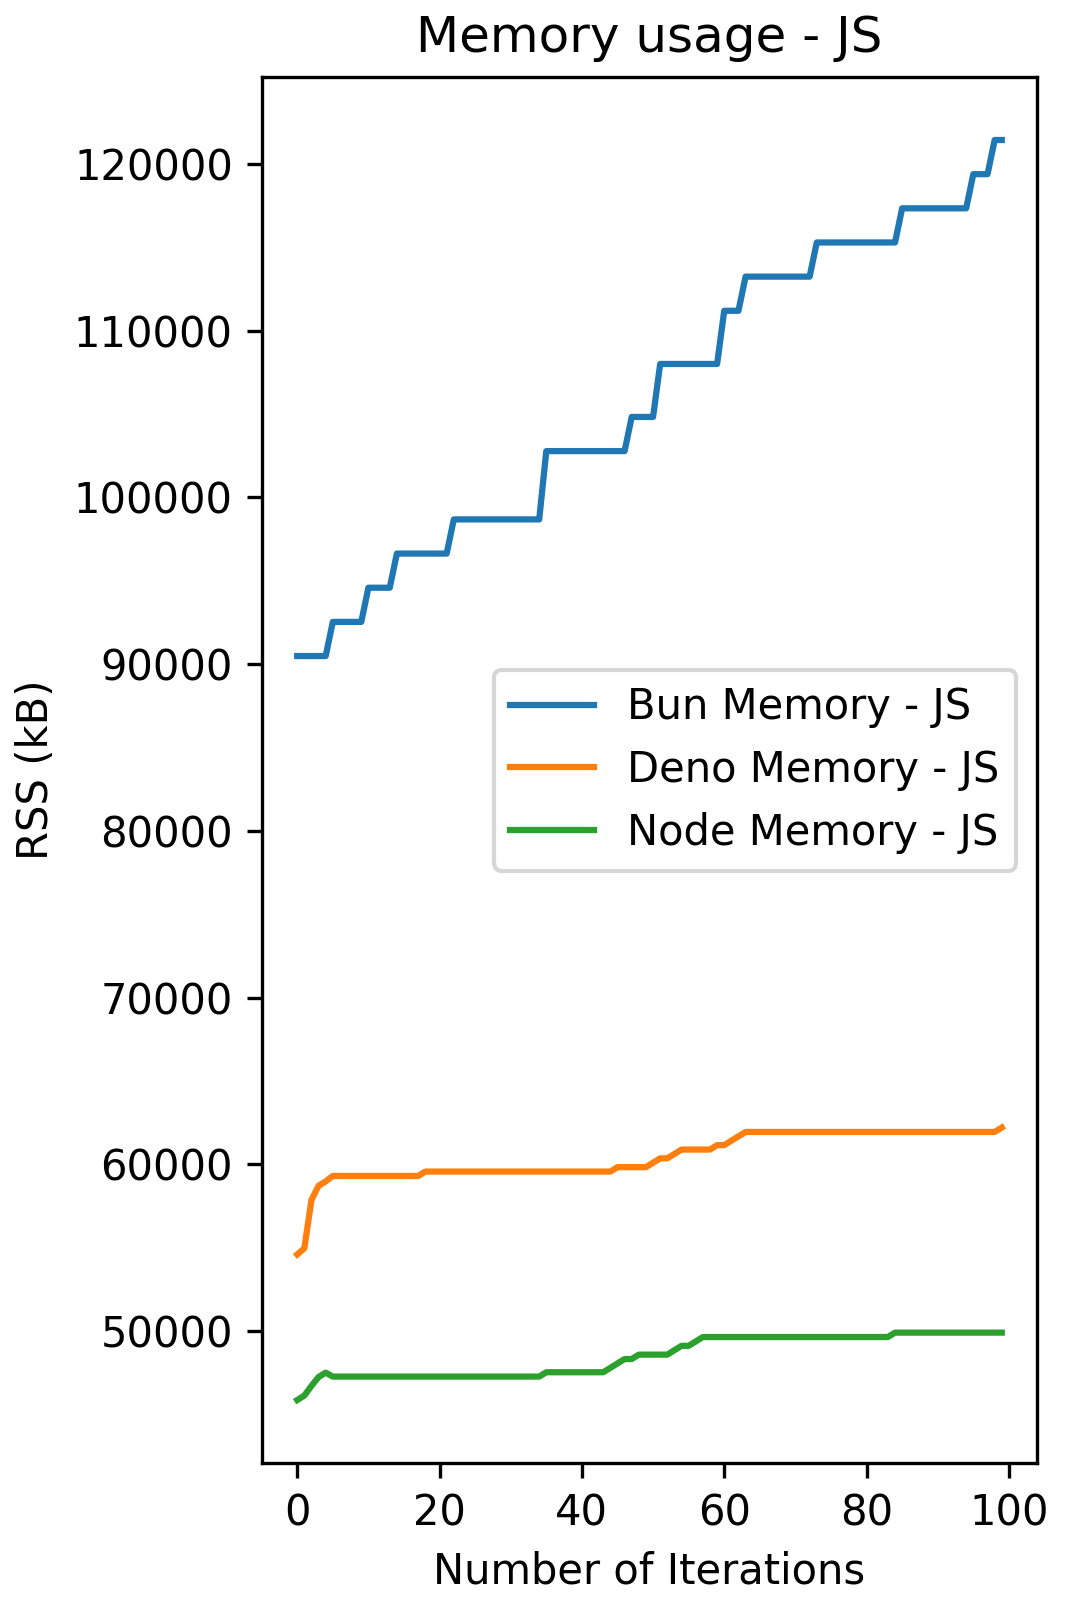
\includegraphics[width=\textwidth]{Figures/sorting/sorting_radix_100_1000_js_memory.png}
    \caption{Zużycie pamięci operacyjnej w kilobajtach (kB)}
    \label{fig:radix_sorting_e1_memory}
  \end{subfigure}
  \caption{Wyniki eksperymentów dla algorytmu sortowania pozycyjnego dla 100 iteracji i 1000 elementów - a) czas wykonania jednorazowego testu w milisekundach, b) ilość zajmowanej pamięci w kilobajtach (kB)}
  \label{fig:radix_sorting_e1}
\end{figure}

Na rysunku \ref{fig:radix_sorting_e1_ts} przedstawiono wyniki eksperymentów dla algorytmu sortowania pozycyjnego dla 100 iteracji i 1000 elementów napisanego w języku TypeScript. Na wykresach przedstawiono czas wykonania jednorazowego testu w milisekundach oraz ilość zajmowanej pamięci w kilobajtach (kB).

\begin{figure}[H]
  \centering
  \begin{subfigure}[b]{0.42\textwidth}
    \centering
    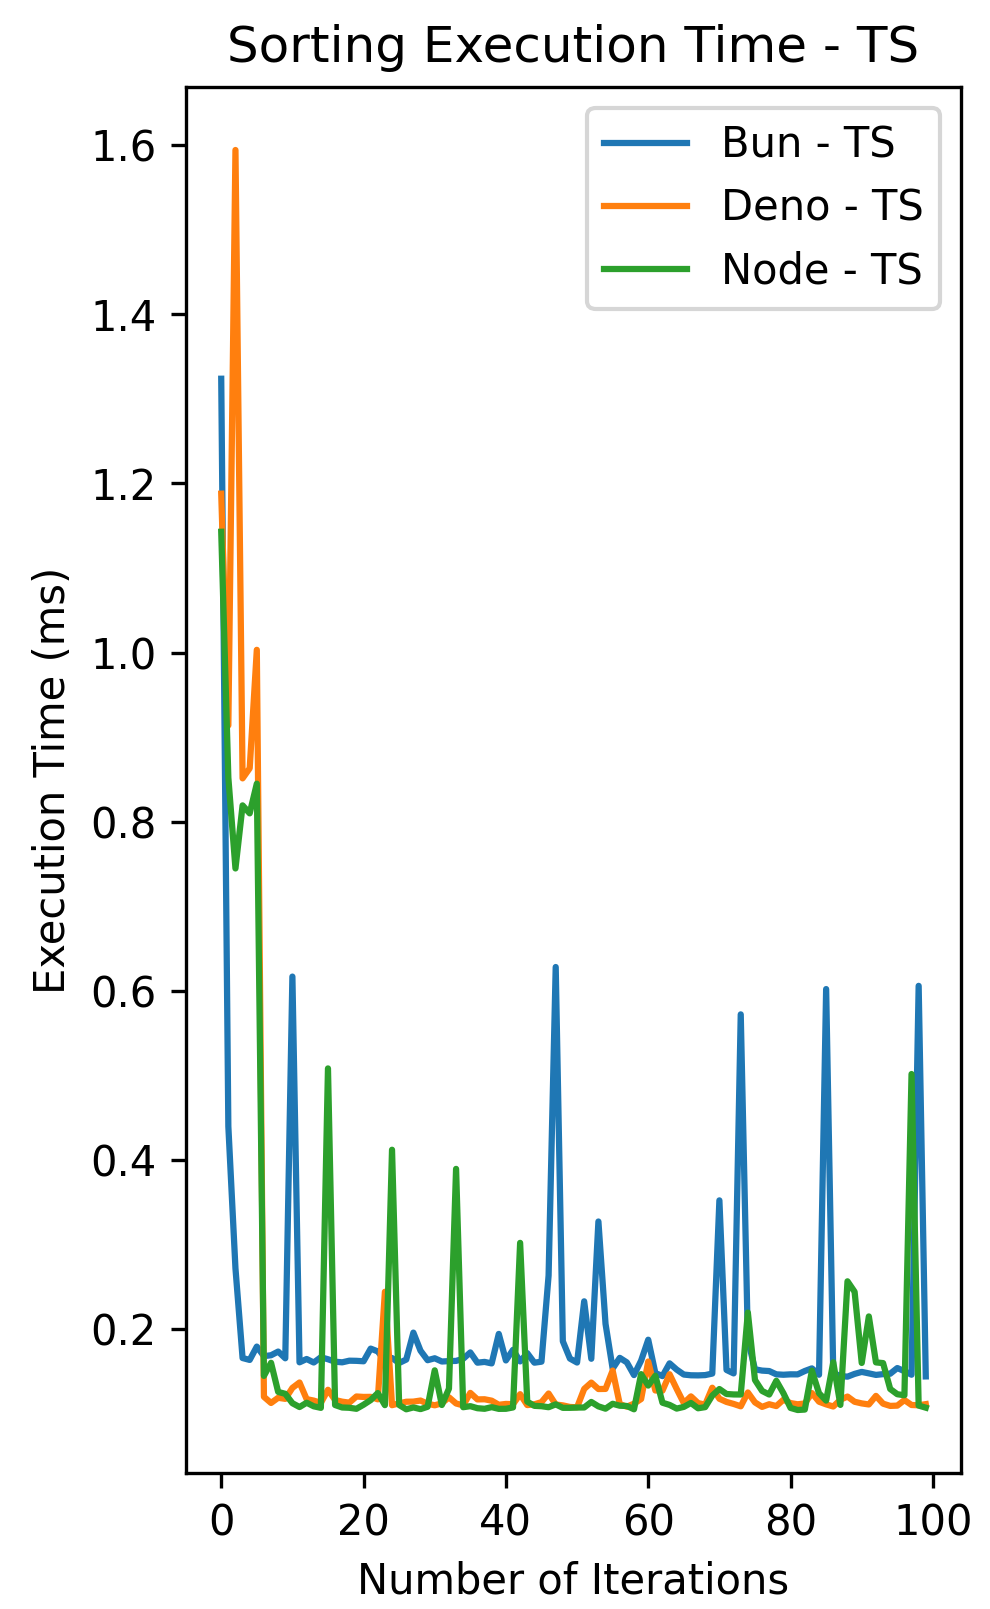
\includegraphics[width=\textwidth]{Figures/sorting/sorting_radix_100_1000_ts_time.png}
    \caption{Czas wykonania testu w milisekundach (ms)}
    \label{fig:radix_sorting_e1_ts_time}
  \end{subfigure}
  \begin{subfigure}[b]{0.42\textwidth}
    \centering
    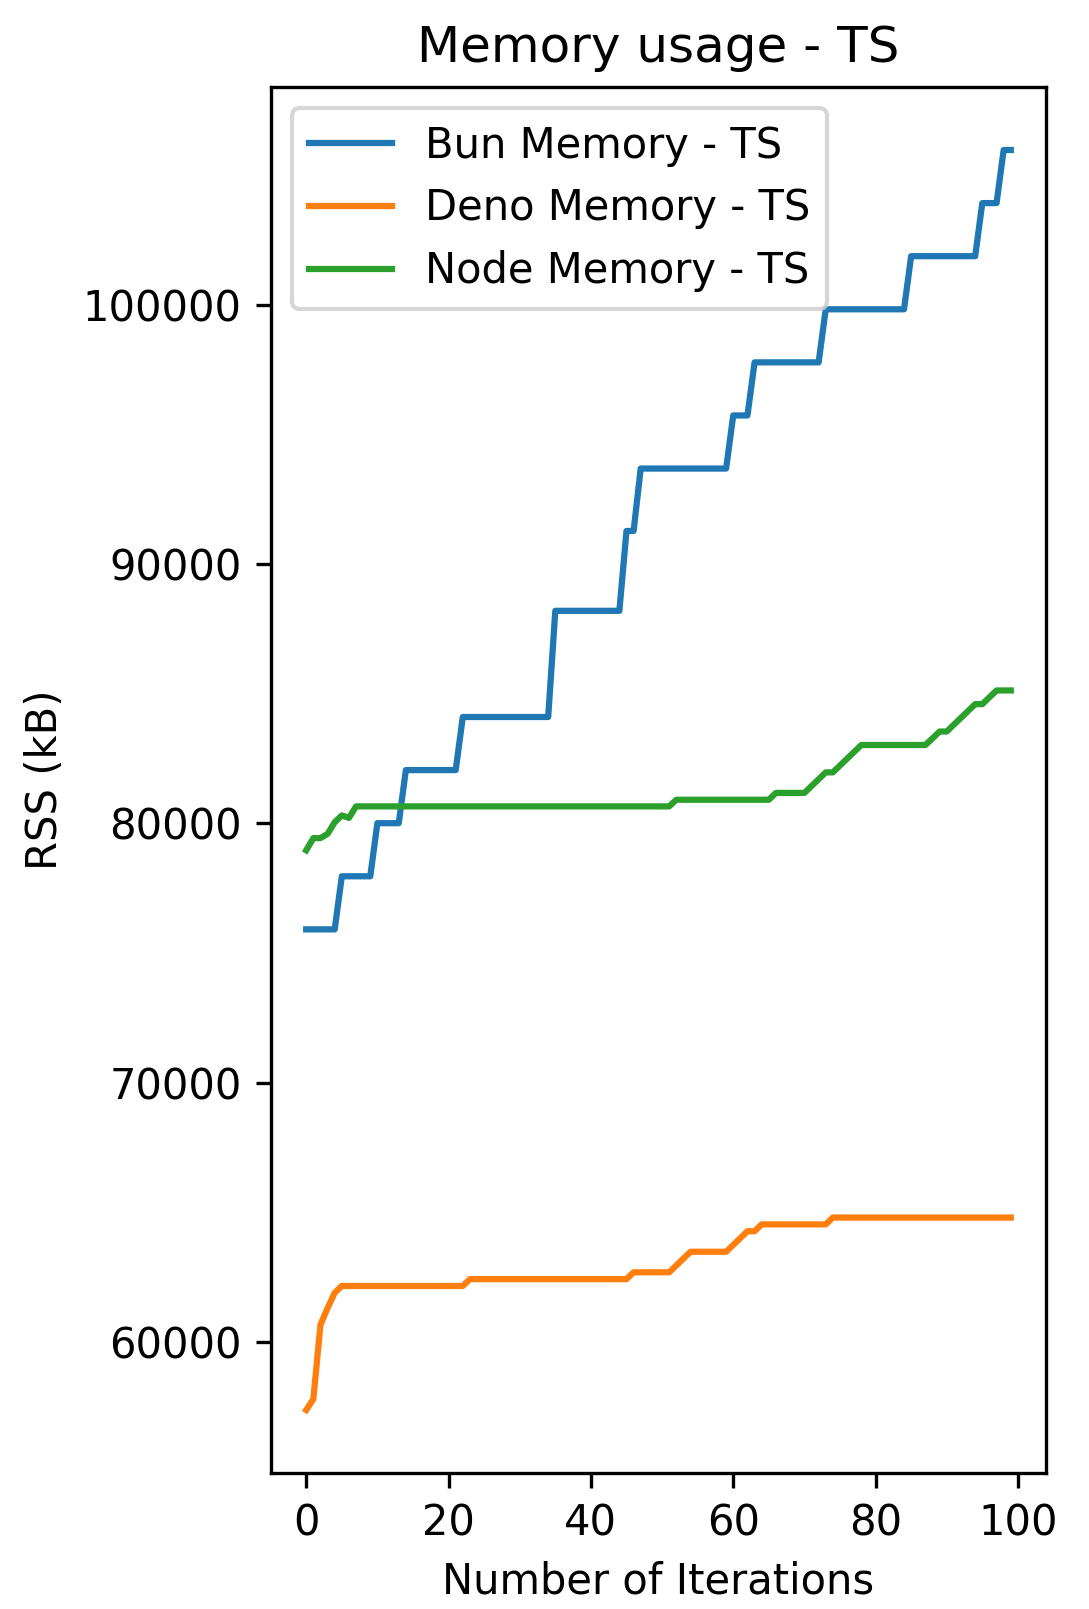
\includegraphics[width=\textwidth]{Figures/sorting/sorting_radix_100_1000_ts_memory.png}
    \caption{Zużycie pamięci operacyjnej w kilobajtach (kB)}
    \label{fig:radix_sorting_e1_ts_memory}
  \end{subfigure}
  \caption{Wyniki eksperymentów dla algorytmu sortowania pozycyjnego dla 100 iteracji i 1000 elementów - a) czas wykonania jednorazowego testu w milisekundach, b) ilość zajmowanej pamięci w kilobajtach (kB)}
  \label{fig:radix_sorting_e1_ts}
\end{figure}

Na rysunku \ref{fig:radix_sorting_e2} przedstawiono wyniki eksperymentów dla algorytmu sortowania pozycyjnego dla 1000 iteracji i 1000 elementów napisanego w języku JavaScript. Na wykresach przedstawiono czas wykonania jednorazowego testu w milisekundach oraz ilość zajmowanej pamięci w kilobajtach (kB).

\begin{figure}[H]
  \centering
  \begin{subfigure}[b]{0.42\textwidth}
    \centering
    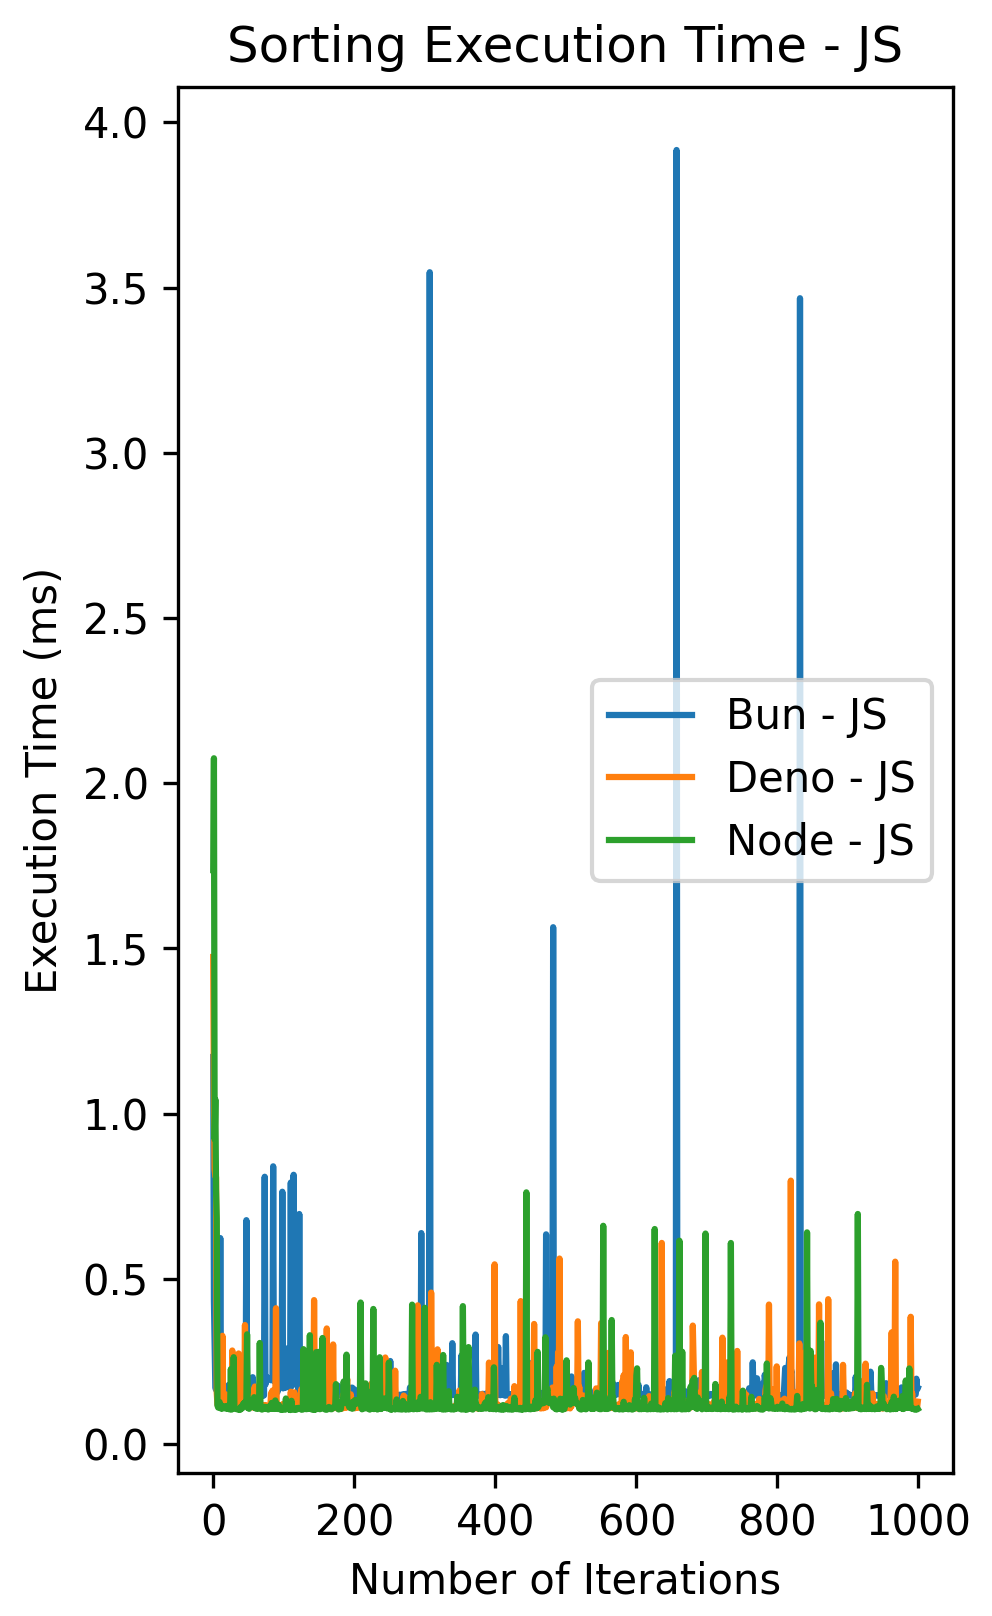
\includegraphics[width=\textwidth]{Figures/sorting/sorting_radix_1000_1000_js_time.png}
    \caption{Czas wykonania testu w milisekundach (ms)}
    \label{fig:radix_sorting_e2_time}
  \end{subfigure}
  \begin{subfigure}[b]{0.42\textwidth}
    \centering
    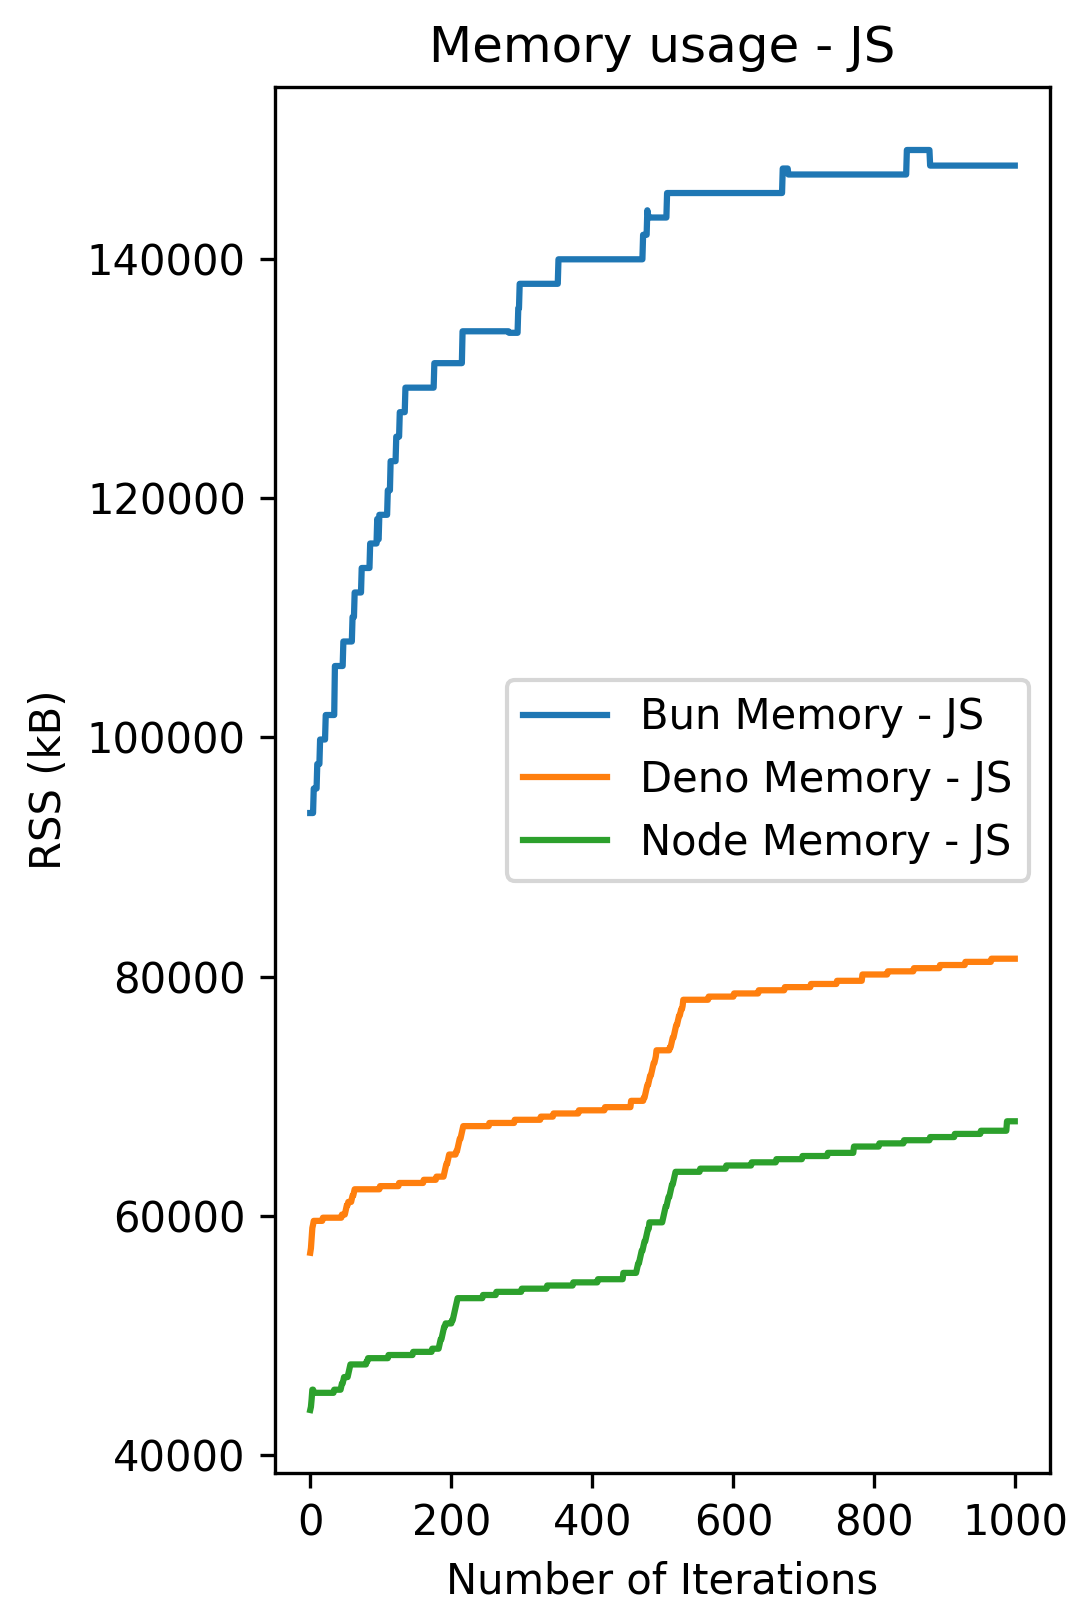
\includegraphics[width=\textwidth]{Figures/sorting/sorting_radix_1000_1000_js_memory.png}
    \caption{Zużycie pamięci operacyjnej w kilobajtach (kB)}
    \label{fig:radix_sorting_e2_memory}
  \end{subfigure}
  \caption{Wyniki eksperymentów dla algorytmu sortowania pozycyjnego dla 1000 iteracji i 10000 elementów - a) czas wykonania jednorazowego testu w milisekundach, b) ilość zajmowanej pamięci w kilobajtach (kB)}
  \label{fig:radix_sorting_e2}
\end{figure}

Na rysunku \ref{fig:radix_sorting_e2_ts} przedstawiono wyniki eksperymentów dla algorytmu sortowania pozycyjnego dla 1000 iteracji i 1000 elementów napisanego w języku TypeScript. Na wykresach przedstawiono czas wykonania jednorazowego testu w milisekundach oraz ilość zajmowanej pamięci w kilobajtach (kB).

\begin{figure}[H]
  \centering
  \begin{subfigure}[b]{0.42\textwidth}
    \centering
    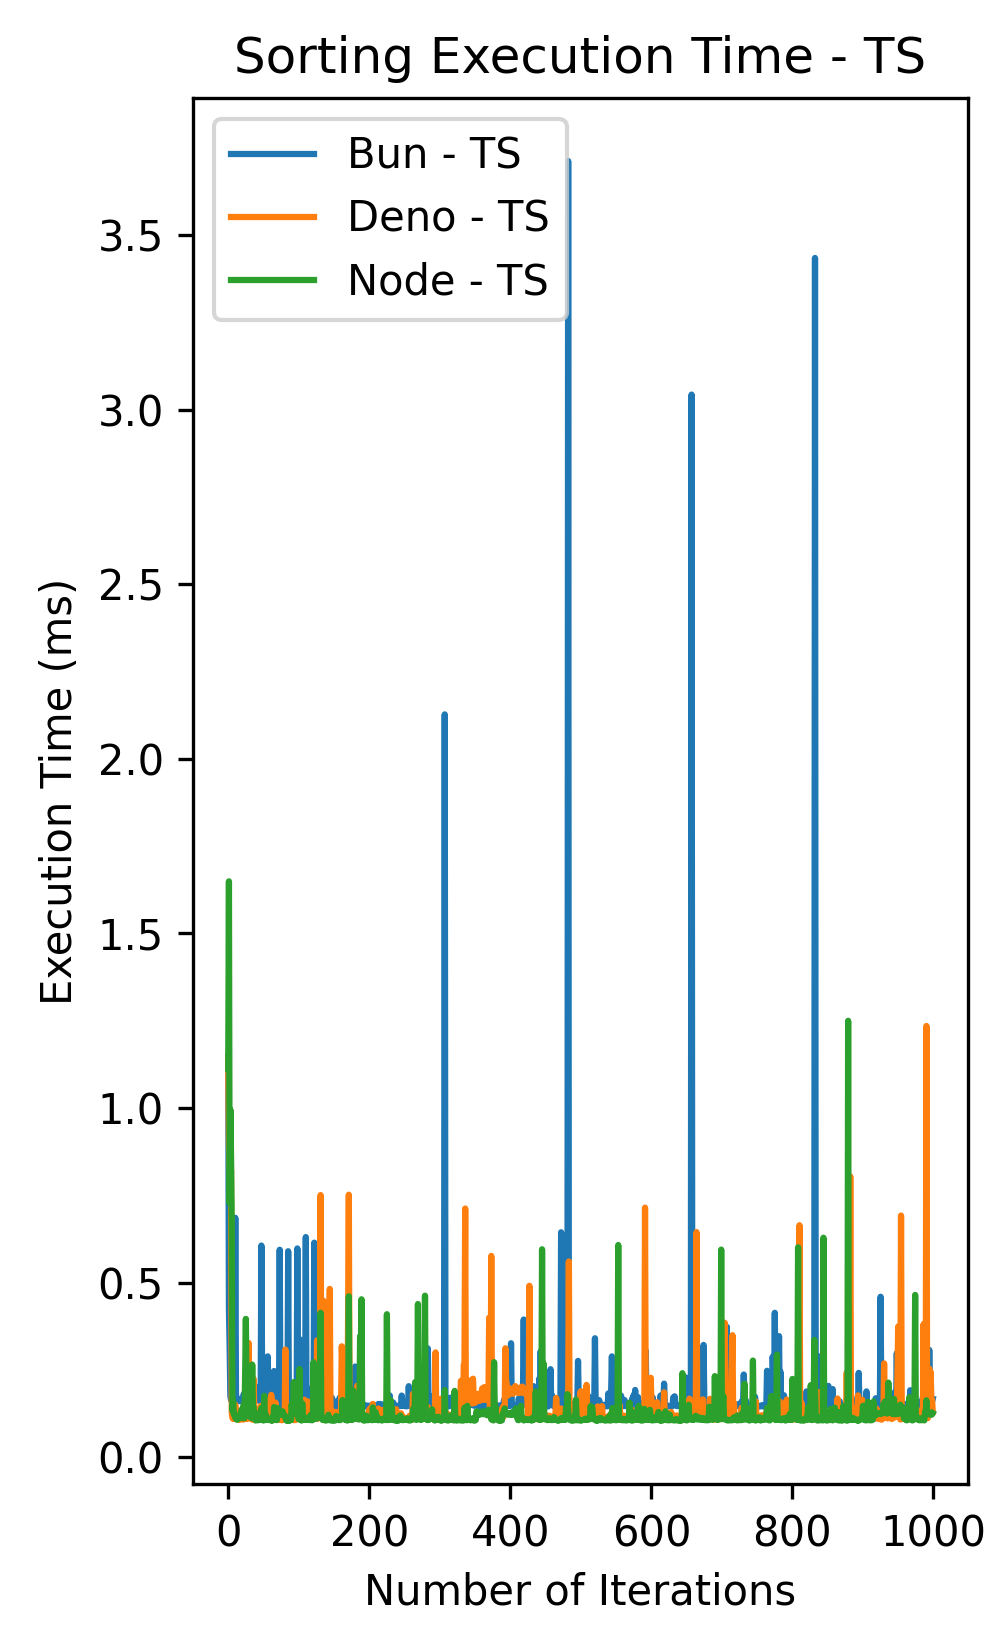
\includegraphics[width=\textwidth]{Figures/sorting/sorting_radix_1000_1000_ts_time.png}
    \caption{Czas wykonania testu w milisekundach (ms)}
    \label{fig:radix_sorting_e2_ts_time}
  \end{subfigure}
  \begin{subfigure}[b]{0.42\textwidth}
    \centering
    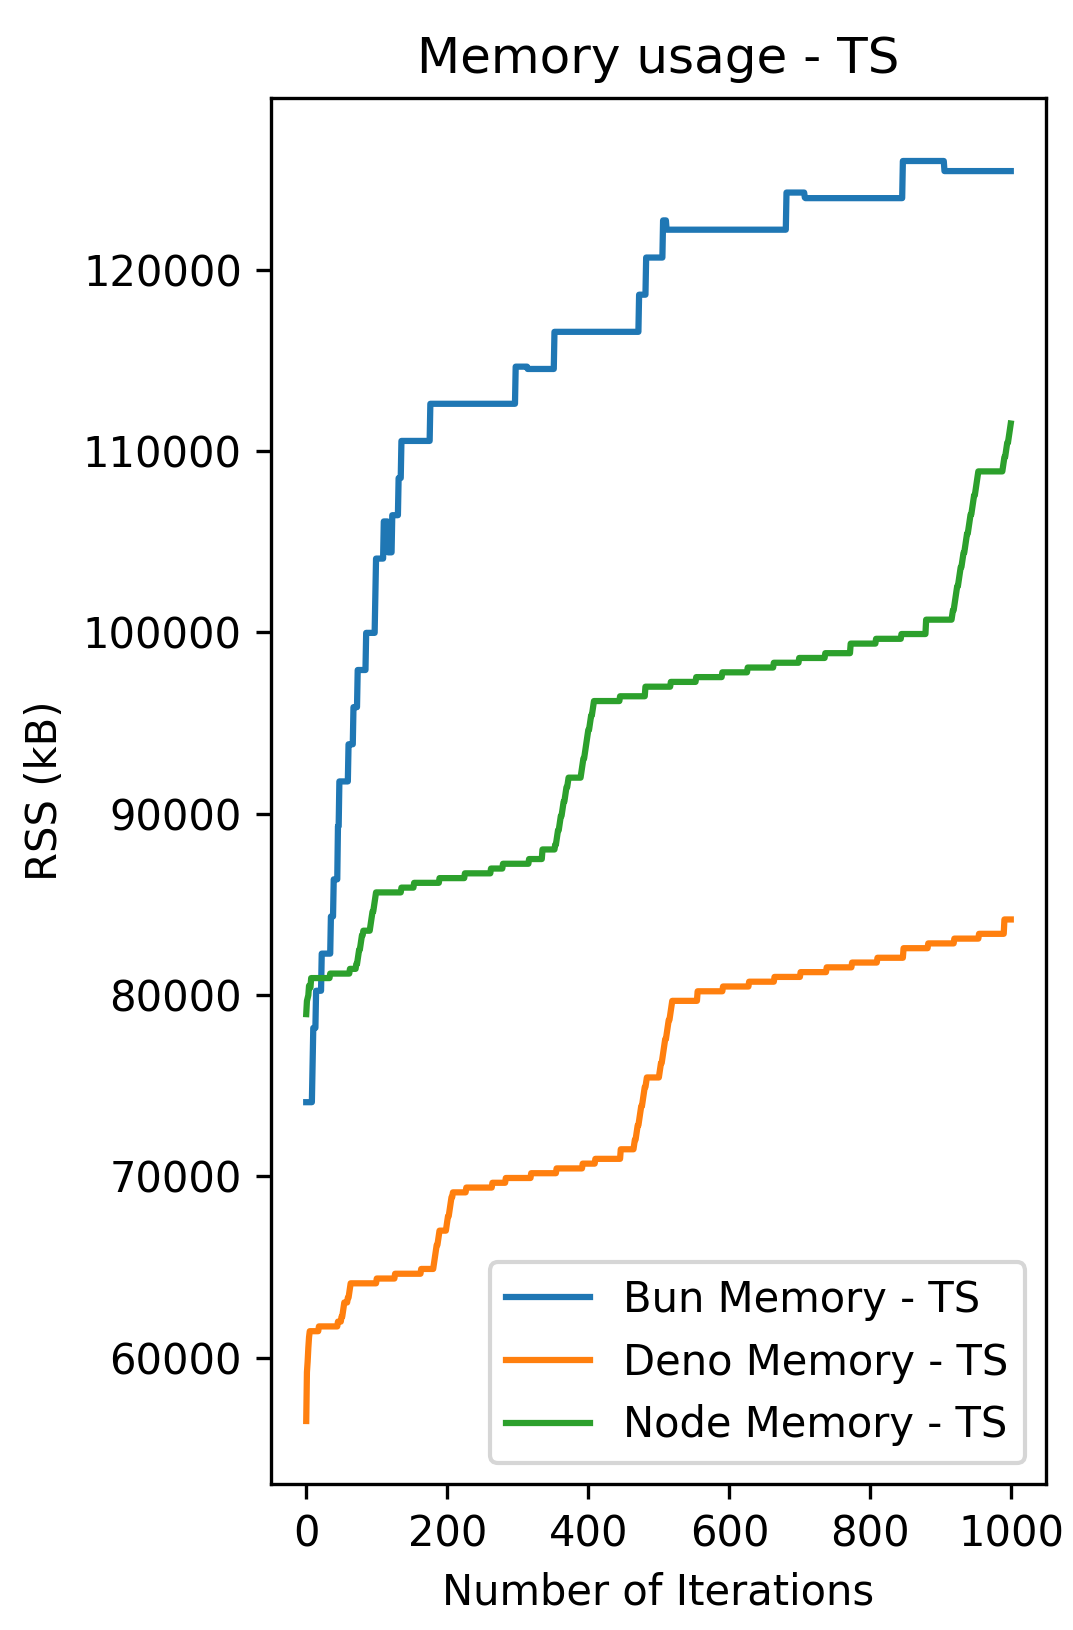
\includegraphics[width=\textwidth]{Figures/sorting/sorting_radix_1000_1000_ts_memory.png}
    \caption{Zużycie pamięci operacyjnej w kilobajtach (kB)}
    \label{fig:radix_sorting_e2_ts_memory}
  \end{subfigure}
  \caption{Wyniki eksperymentów dla algorytmu sortowania pozycyjnego dla 1000 iteracji i 1000 elementów - a) czas wykonania jednorazowego testu w milisekundach, b) ilość zajmowanej pamięci w kilobajtach (kB)}
  \label{fig:radix_sorting_e2_ts}
\end{figure}

Na rysunku \ref{fig:radix_sorting_e3} przedstawiono wyniki eksperymentów dla algorytmu sortowania dla 100 iteracji i 10000 elementów napisanego w języku JavaScript. Na wykresach przedstawiono czas wykonania jednorazowego testu w milisekundach oraz ilość zajmowanej pamięci w kilobajtach (kB).

\begin{figure}[H]
  \centering
  \begin{subfigure}[b]{0.42\textwidth}
    \centering
    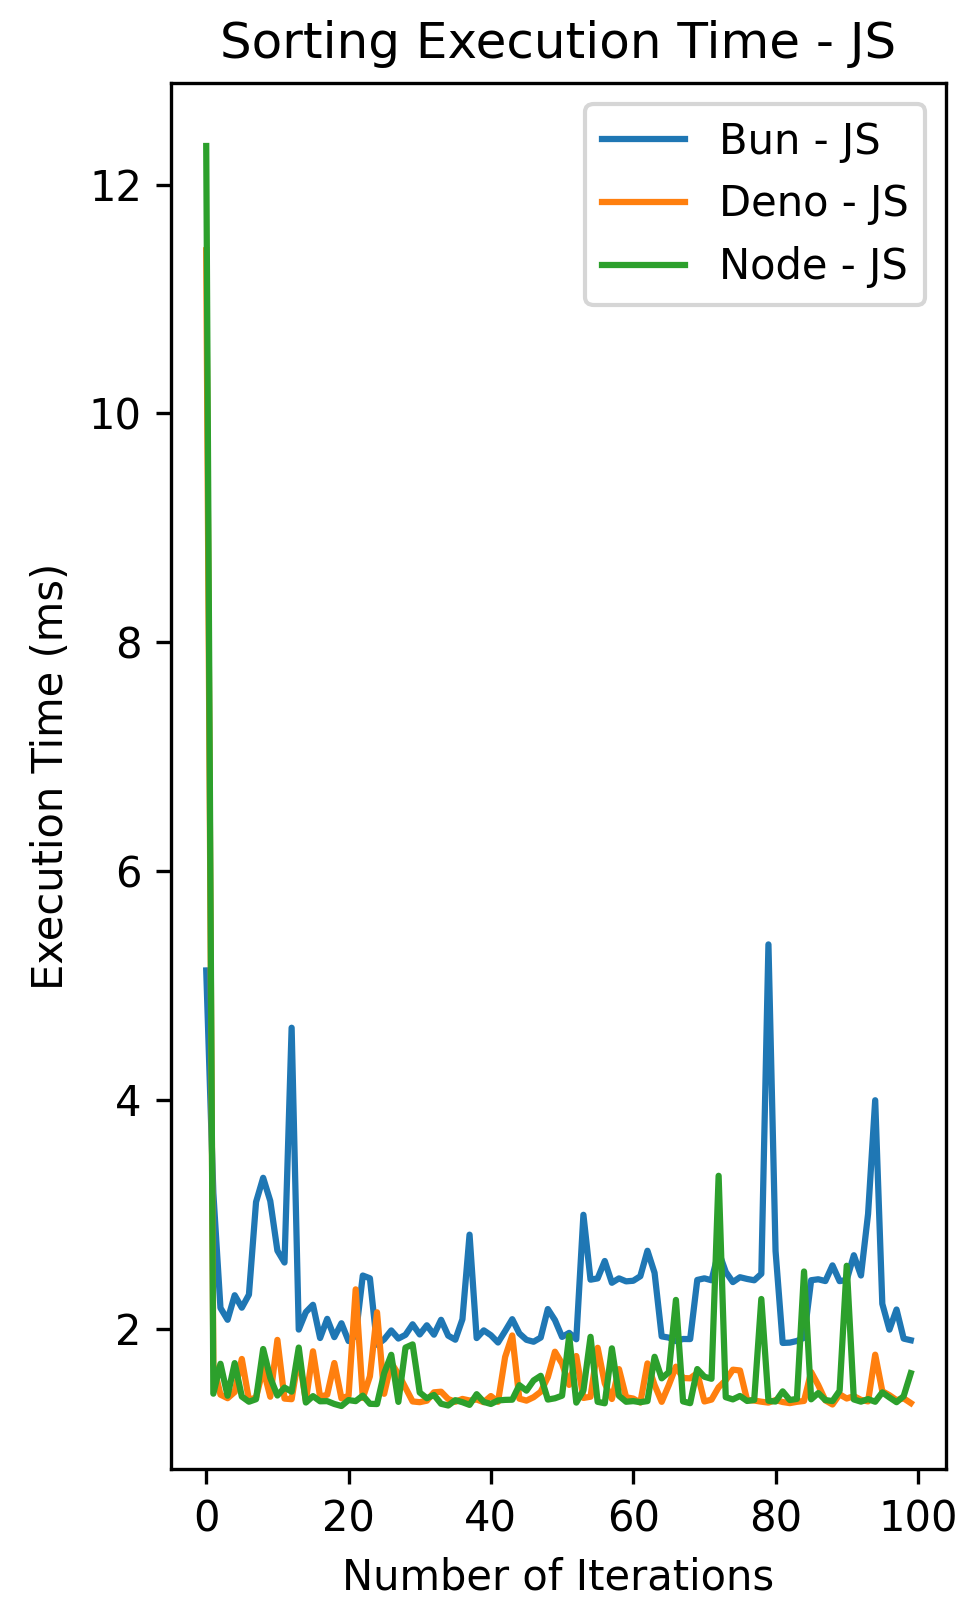
\includegraphics[width=\textwidth]{Figures/sorting/sorting_radix_100_10000_js_time.png}
    \caption{Czas wykonania testu w milisekundach (ms)}
    \label{fig:radix_sorting_e3_time}
  \end{subfigure}
  \begin{subfigure}[b]{0.42\textwidth}
    \centering
    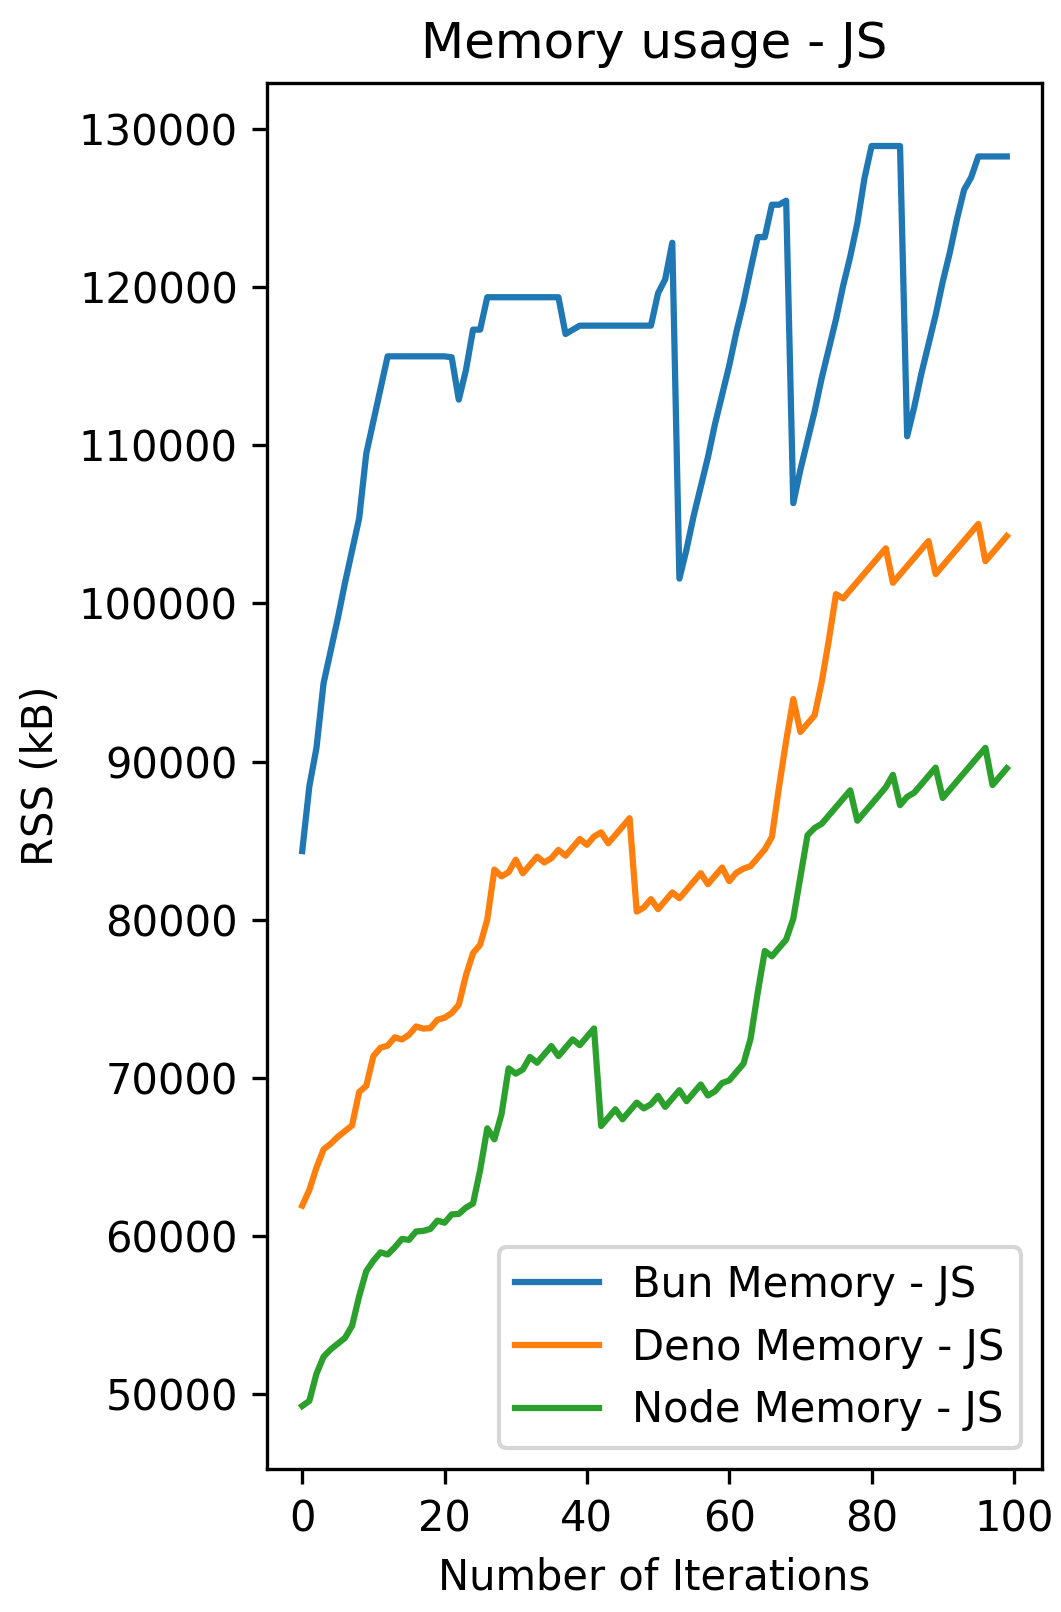
\includegraphics[width=\textwidth]{Figures/sorting/sorting_radix_100_10000_js_memory.png}
    \caption{Zużycie pamięci operacyjnej w kilobajtach (kB)}
    \label{fig:radix_sorting_e3_memory}
  \end{subfigure}
  \caption{Wyniki eksperymentów dla algorytmu sortowania pozycyjnego dla 100 iteracji i 10000 elementów - a) czas wykonania jednorazowego testu w milisekundach, b) ilość zajmowanej pamięci w kilobajtach (kB)}
  \label{fig:radix_sorting_e3}
\end{figure}

Na rysunku \ref{fig:radix_sorting_e3_ts} przedstawiono wyniki eksperymentów dla algorytmu sortowania pozycyjnego dla 100 iteracji i 10000 elementów napisanego w języku TypeScript. Na wykresach przedstawiono czas wykonania jednorazowego testu w milisekundach oraz ilość zajmowanej pamięci w kilobajtach (kB).

\begin{figure}[H]
  \centering
  \begin{subfigure}[b]{0.42\textwidth}
    \centering
    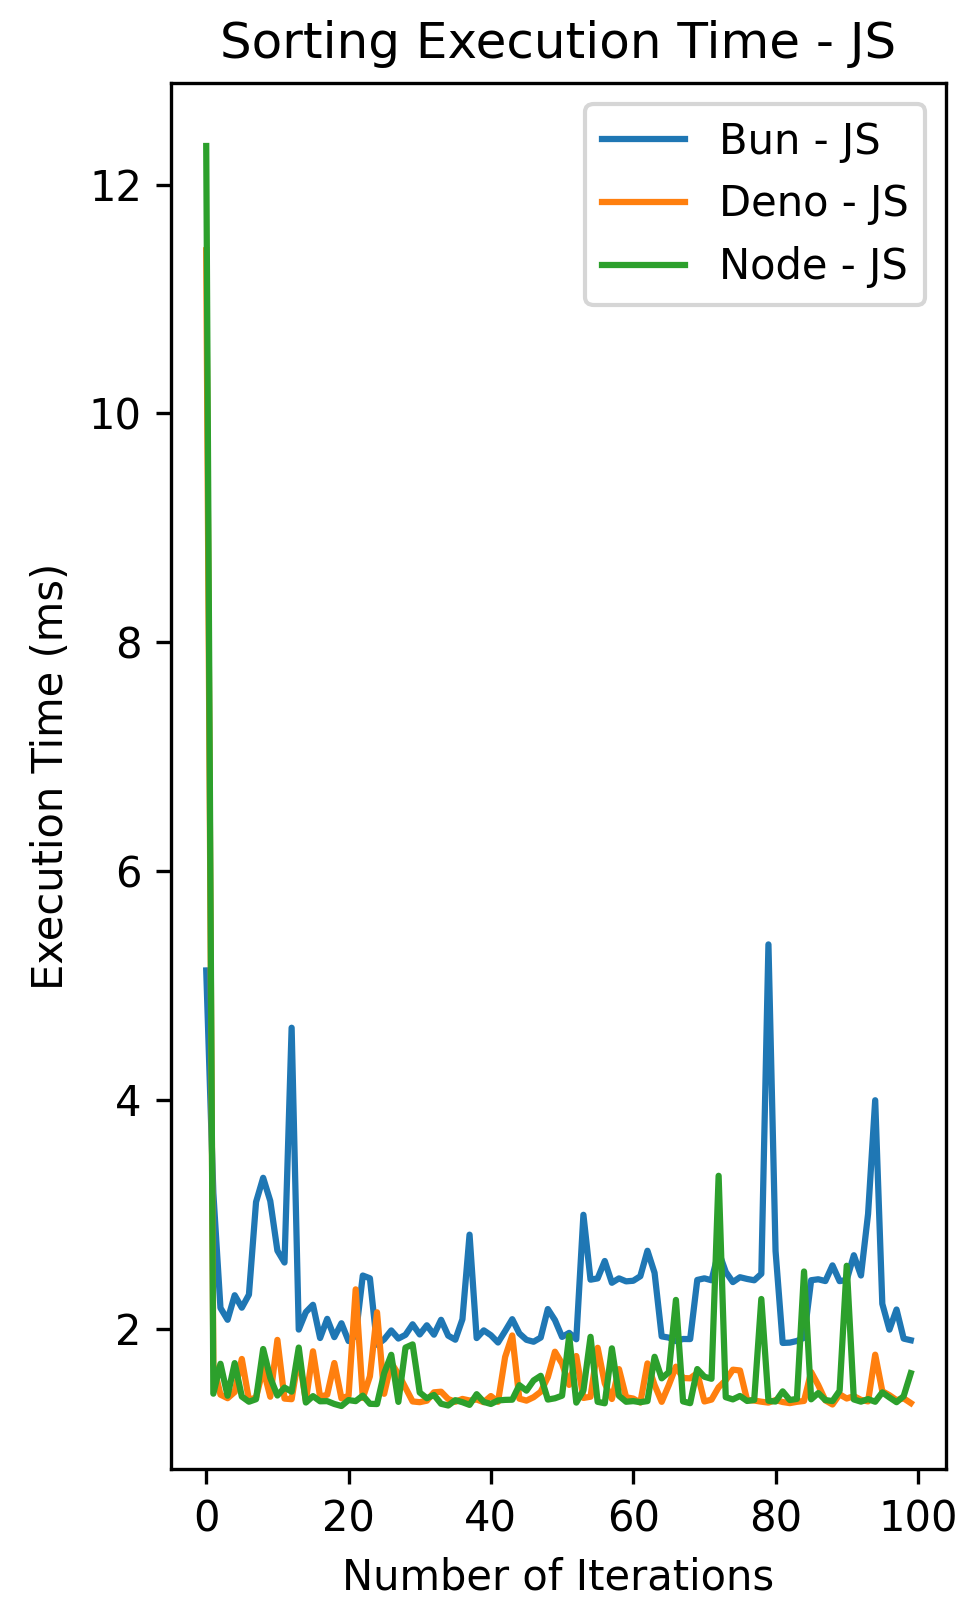
\includegraphics[width=\textwidth]{Figures/sorting/sorting_radix_100_10000_js_time.png}
    \caption{Czas wykonania testu w milisekundach (ms)}
    \label{fig:radix_sorting_e3_ts_time}
  \end{subfigure}
  \begin{subfigure}[b]{0.42\textwidth}
    \centering
    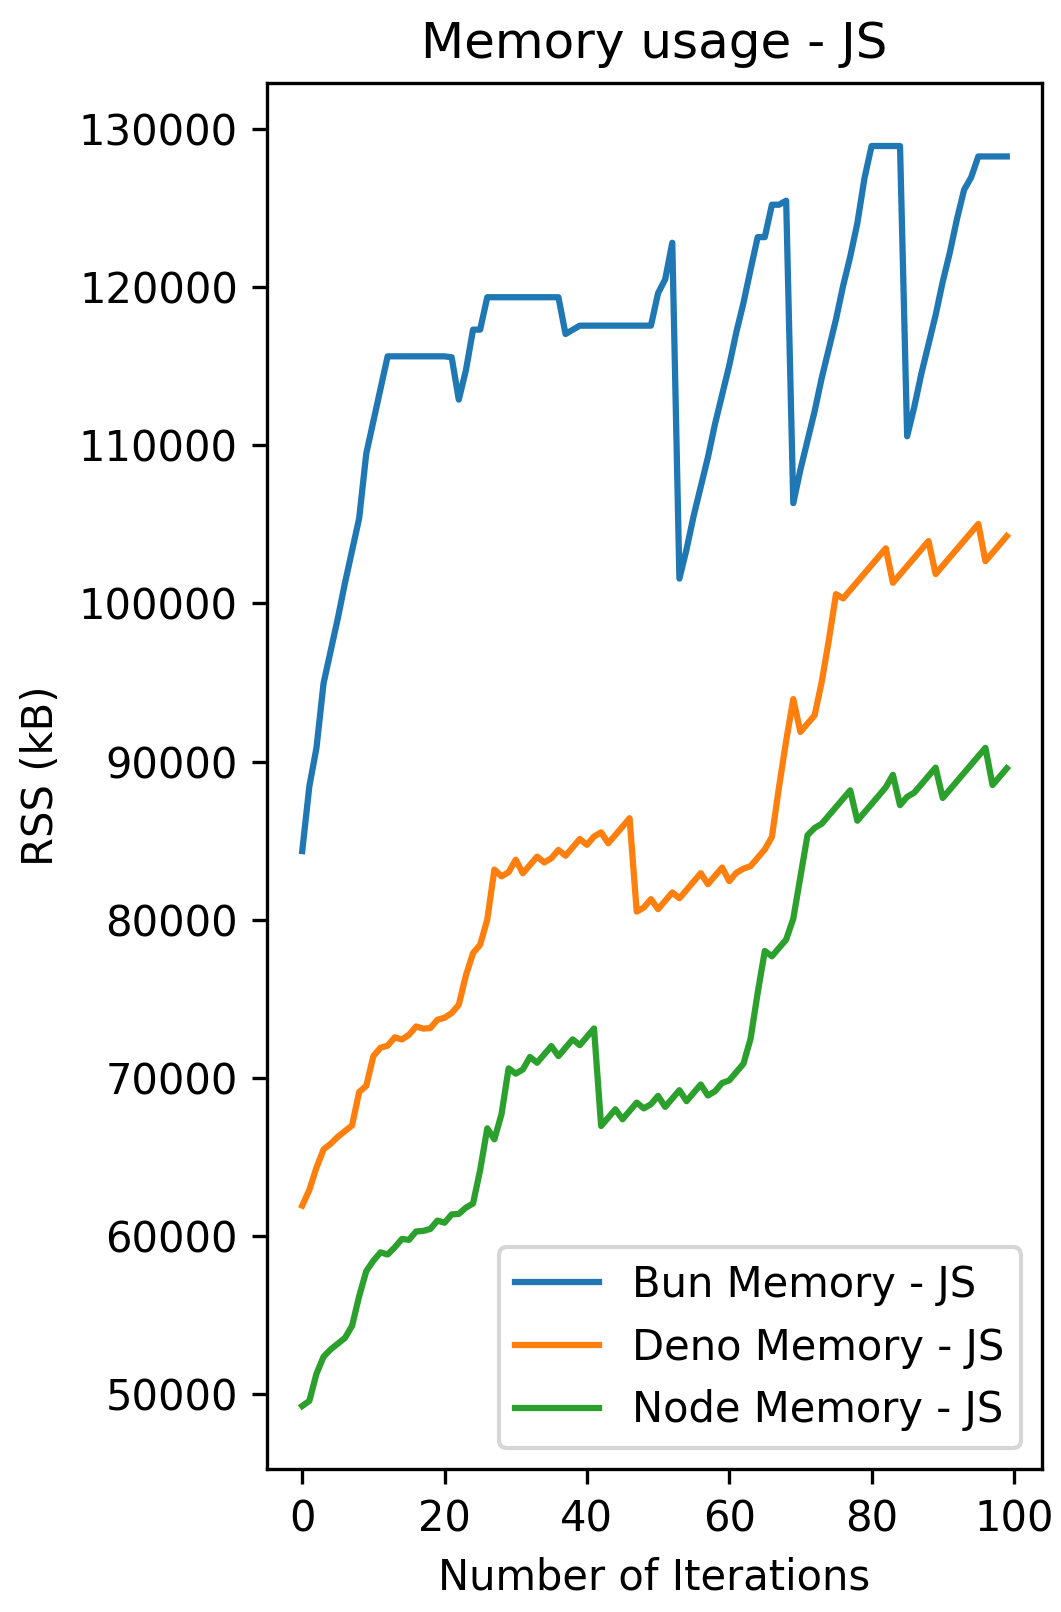
\includegraphics[width=\textwidth]{Figures/sorting/sorting_radix_100_10000_js_memory.png}
    \caption{Zużycie pamięci operacyjnej w kilobajtach (kB)}
    \label{fig:radix_sorting_e3_ts_memory}
  \end{subfigure}
  \hfill
  \caption{Wyniki eksperymentów dla algorytmu sortowania pozycyjnego dla 100 iteracji i 1000 elementów - a) czas wykonania jednorazowego testu w milisekundach, b) ilość zajmowanej pamięci w kilobajtach (kB)}
  \label{fig:radix_sorting_e3_ts}
\end{figure}

Na rysunku \ref{fig:radix_sorting_e4} przedstawiono wyniki eksperymentów dla algorytmu sortowania pozycyjnego dla 1000 iteracji i 10000 elementów napisanego w języku JavaScript. Na wykresach przedstawiono czas wykonania jednorazowego testu w milisekundach oraz ilość zajmowanej pamięci w kilobajtach (kB).

\begin{figure}[H]
  \centering
  \begin{subfigure}[b]{0.42\textwidth}
    \centering
    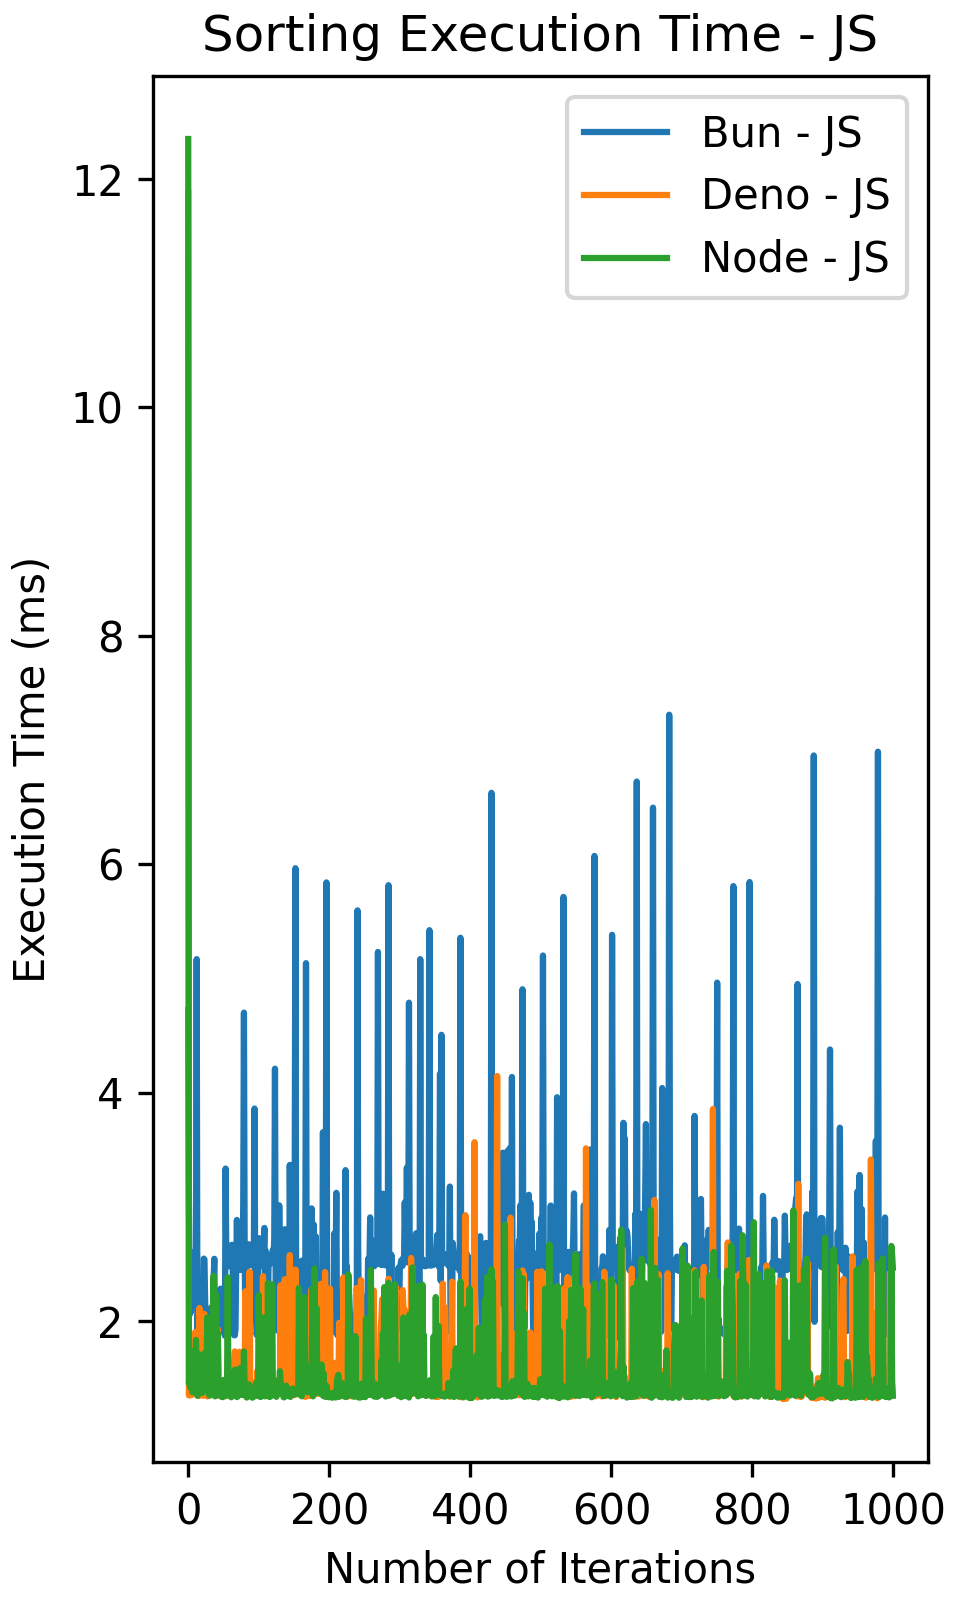
\includegraphics[width=\textwidth]{Figures/sorting/sorting_radix_1000_10000_js_time.png}
    \caption{Czas wykonania testu w milisekundach (ms)}
    \label{fig:radix_sorting_e4_time}
  \end{subfigure}
  \begin{subfigure}[b]{0.42\textwidth}
    \centering
    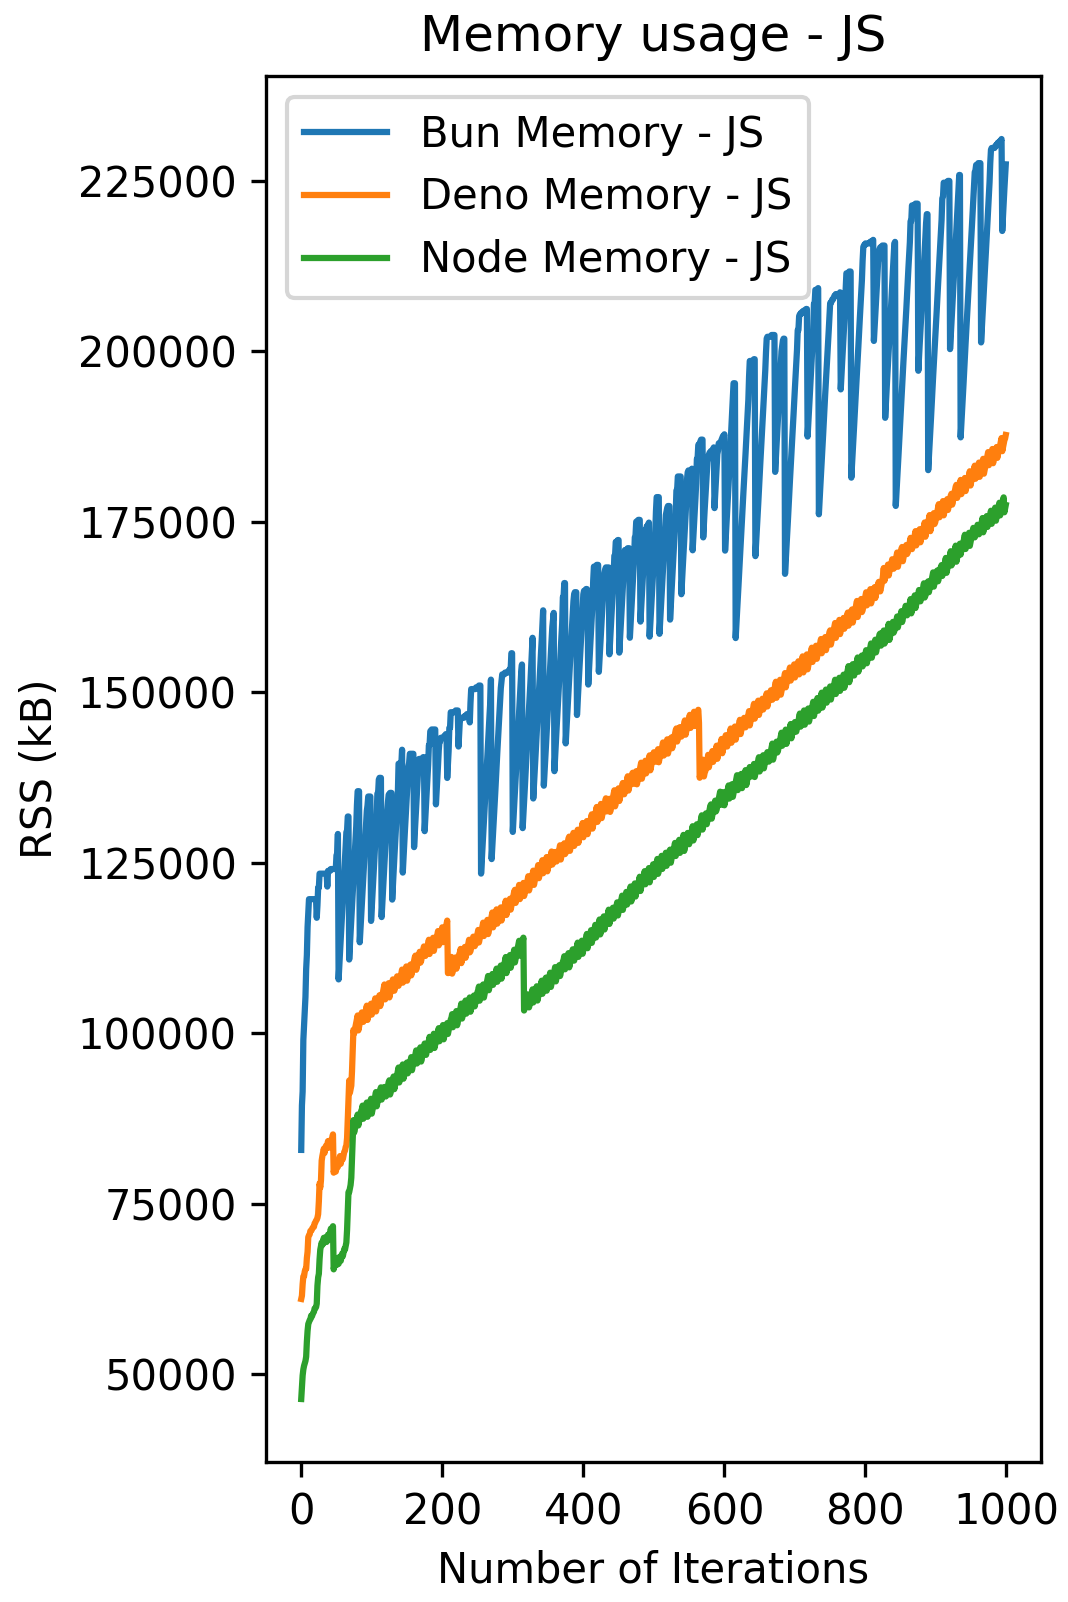
\includegraphics[width=\textwidth]{Figures/sorting/sorting_radix_1000_10000_js_memory.png}
    \caption{Zużycie pamięci operacyjnej w kilobajtach (kB)}
    \label{fig:radix_sorting_e4_memory}
  \end{subfigure}
  \hfill
  \caption{Wyniki eksperymentów dla algorytmu sortowania pozycyjnego dla 1000 iteracji i 10000 elementów - a) czas wykonania jednorazowego testu w milisekundach, b) ilość zajmowanej pamięci w kilobajtach (kB)}
  \label{fig:radix_sorting_e4}
\end{figure}

Na rysunku \ref{fig:radix_sorting_e4_ts} przedstawiono wyniki eksperymentów dla algorytmu sortowania pozycyjnego dla 1000 iteracji i 10000 elementów napisanego w języku TypeScript. Na wykresach przedstawiono czas wykonania jednorazowego testu w milisekundach oraz ilość zajmowanej pamięci w kilobajtach (kB).

\begin{figure}[H]
  \centering
  \begin{subfigure}[b]{0.42\textwidth}
    \centering
    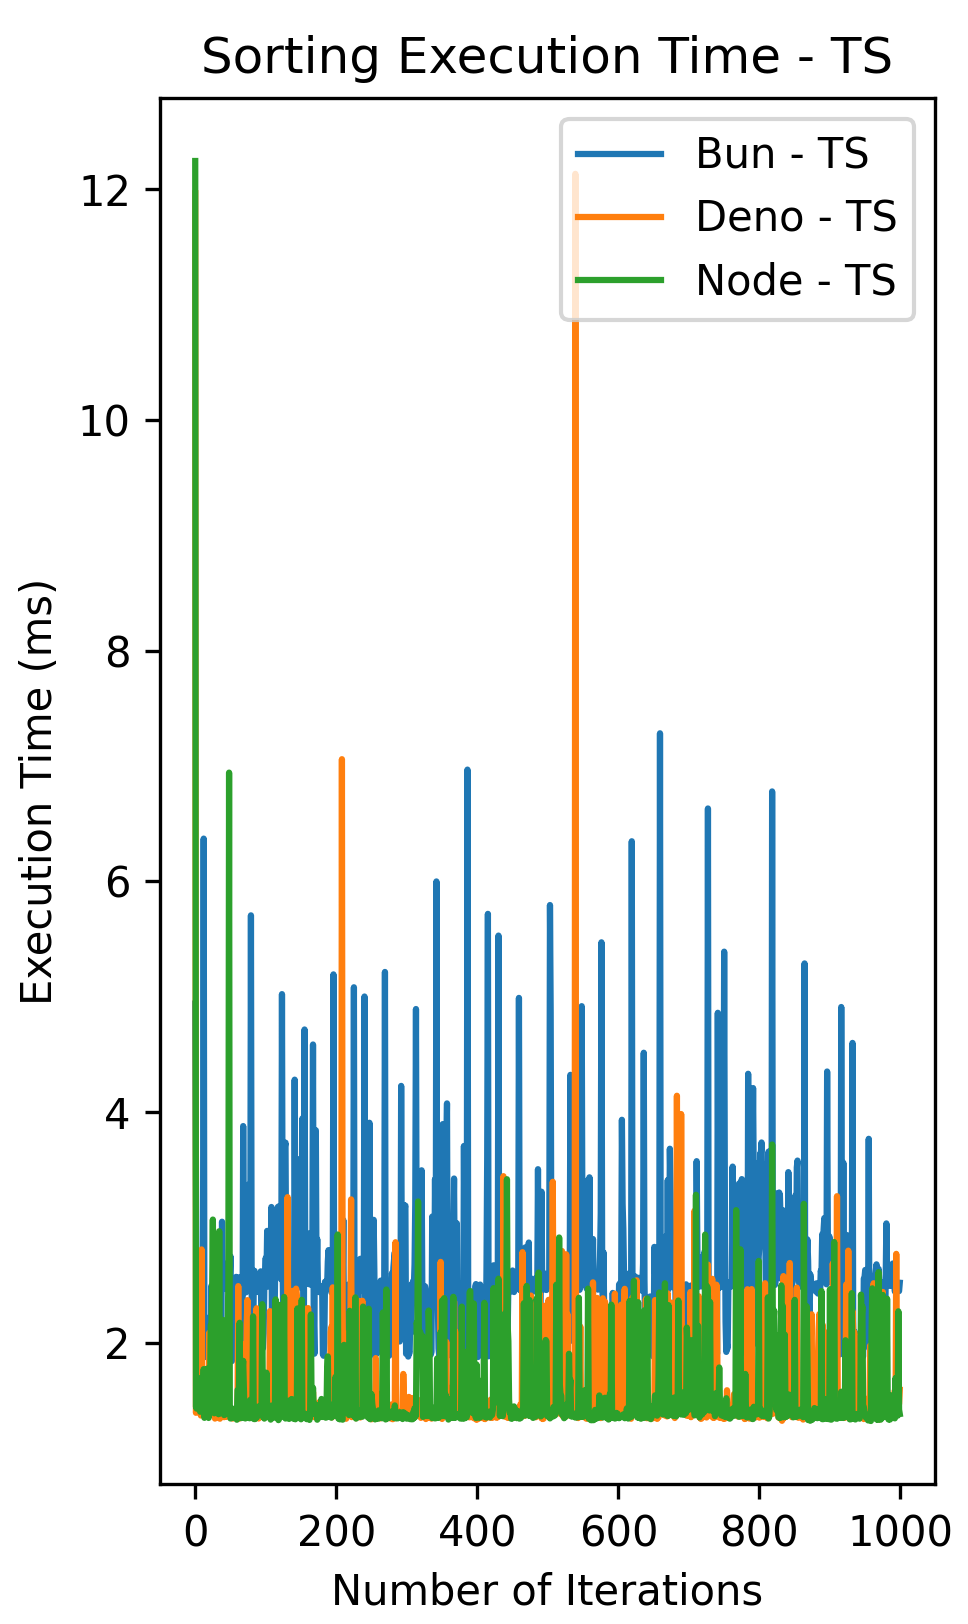
\includegraphics[width=\textwidth]{Figures/sorting/sorting_radix_1000_10000_ts_time.png}
    \caption{Czas wykonania testu w milisekundach (ms)}
    \label{fig:radix_sorting_e4_ts_time}
  \end{subfigure}
  \begin{subfigure}[b]{0.42\textwidth}
    \centering
    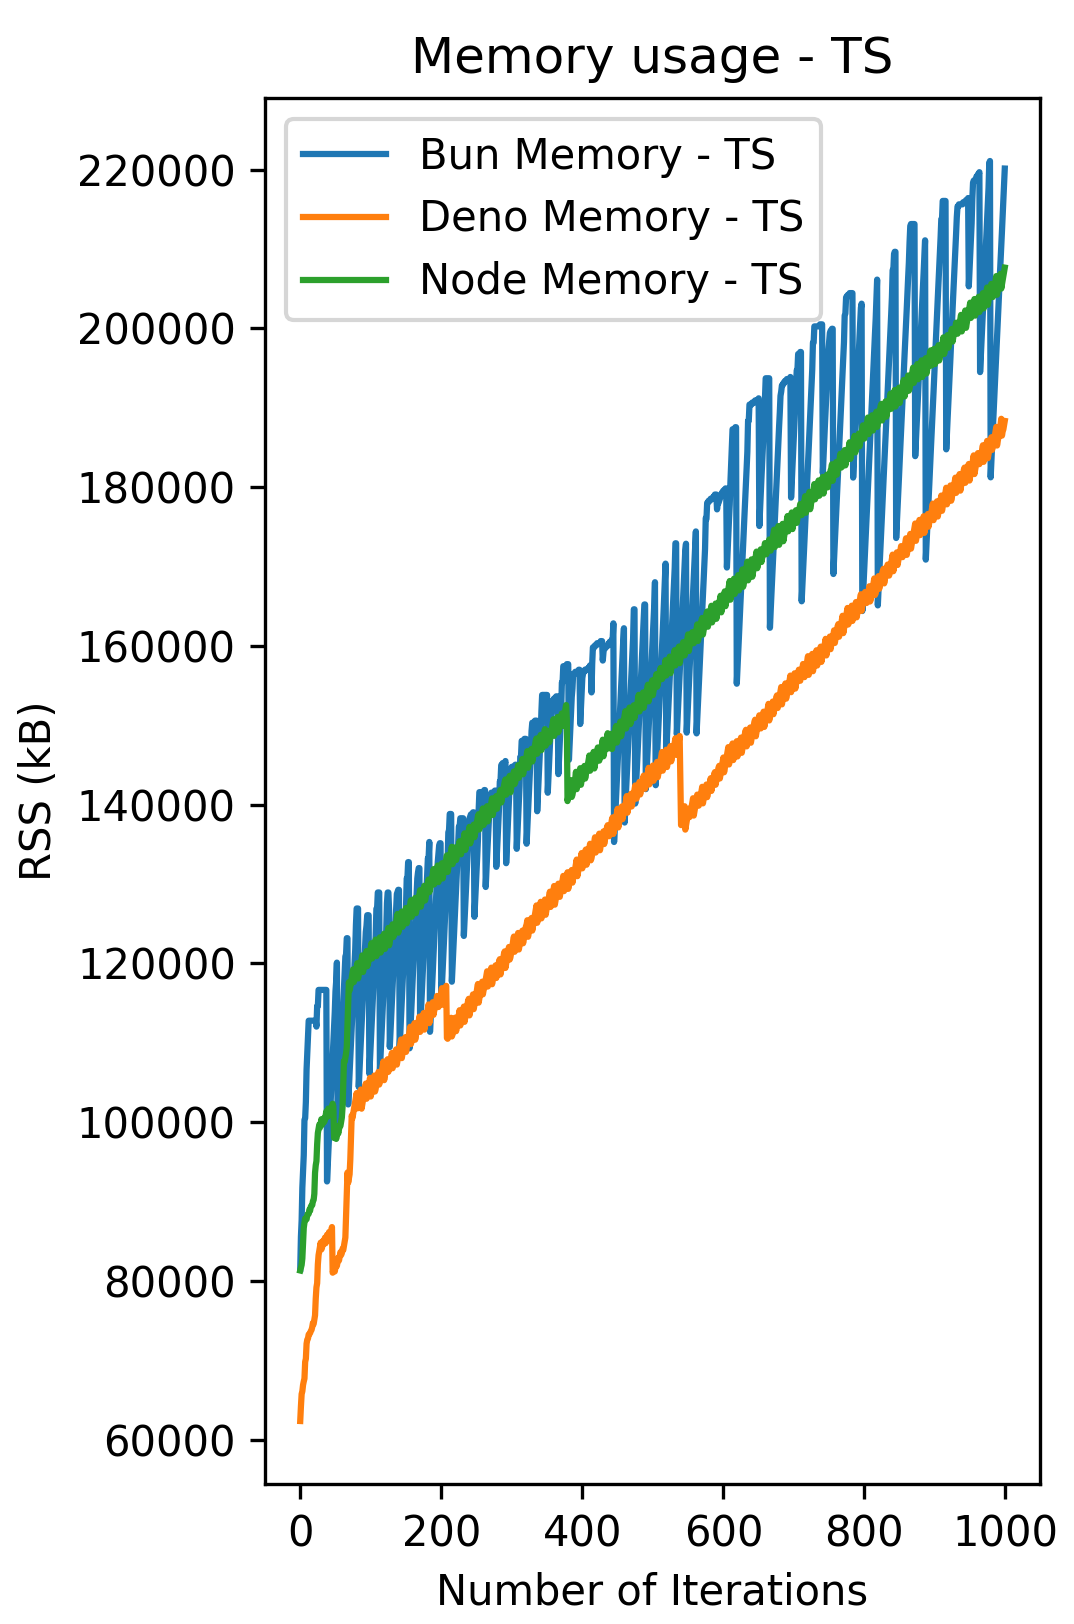
\includegraphics[width=\textwidth]{Figures/sorting/sorting_radix_1000_10000_ts_memory.png}
    \caption{Zużycie pamięci operacyjnej w kilobajtach (kB)}
    \label{fig:radix_sorting_e4_ts_memory}
  \end{subfigure}
  \hfill
  \caption{Wyniki eksperymentów dla algorytmu sortowania pozycyjnego dla 1000 iteracji i 10000 elementów - a) czas wykonania jednorazowego testu w milisekundach, b) ilość zajmowanej pamięci w kilobajtach (kB)}
  \label{fig:radix_sorting_e4_ts}
\end{figure}

\subsection{Algorytmy kodowania}
W celu zbadania wydajności możliwości kodowania dla środowisk, użyto algorytmu kodowania \textit{Base64}, który jest najpopularniejszym algorytmem kodowania wykorzystywanym w aplikacjach webowych. W tabeli \ref{tab:encoding_experiments} przedstawiono liczbę przeprowadzonych eksperymentów, długość kodowanego słowa.

\begin{table}[H]
  \centering
  \caption{Parametry eksperymentów algorytmu kodowania \textit{Base64}}
  \begin{tabular}{|c|c|}
    \hline
    \textbf{Liczba eksperymentów} & \textbf{Długość słowa}\\ \hline
    1000 & 8192 \\ \hline
    100 & 32768 \\ \hline
  \end{tabular}
  \label{tab:encoding_experiments}
\end{table}

\subsubsection{Wyniki}
Na rysunku \ref{fig:encoding_e1_js} przedstawiono wyniki eksperymentów dla operacji kodowania z wykorzystaniem algorytmu kodowania \textit{Base64} dla 100 iteracji i 32768 znaków napisanego w języku JavaScript. Na wykresach przedstawiono czas wykonania jednorazowego testu w milisekundach oraz ilość zajmowanej pamięci w kilobajtach (kB).

\begin{figure}[H]
  \centering
  \begin{subfigure}[b]{0.42\textwidth}
    \centering
    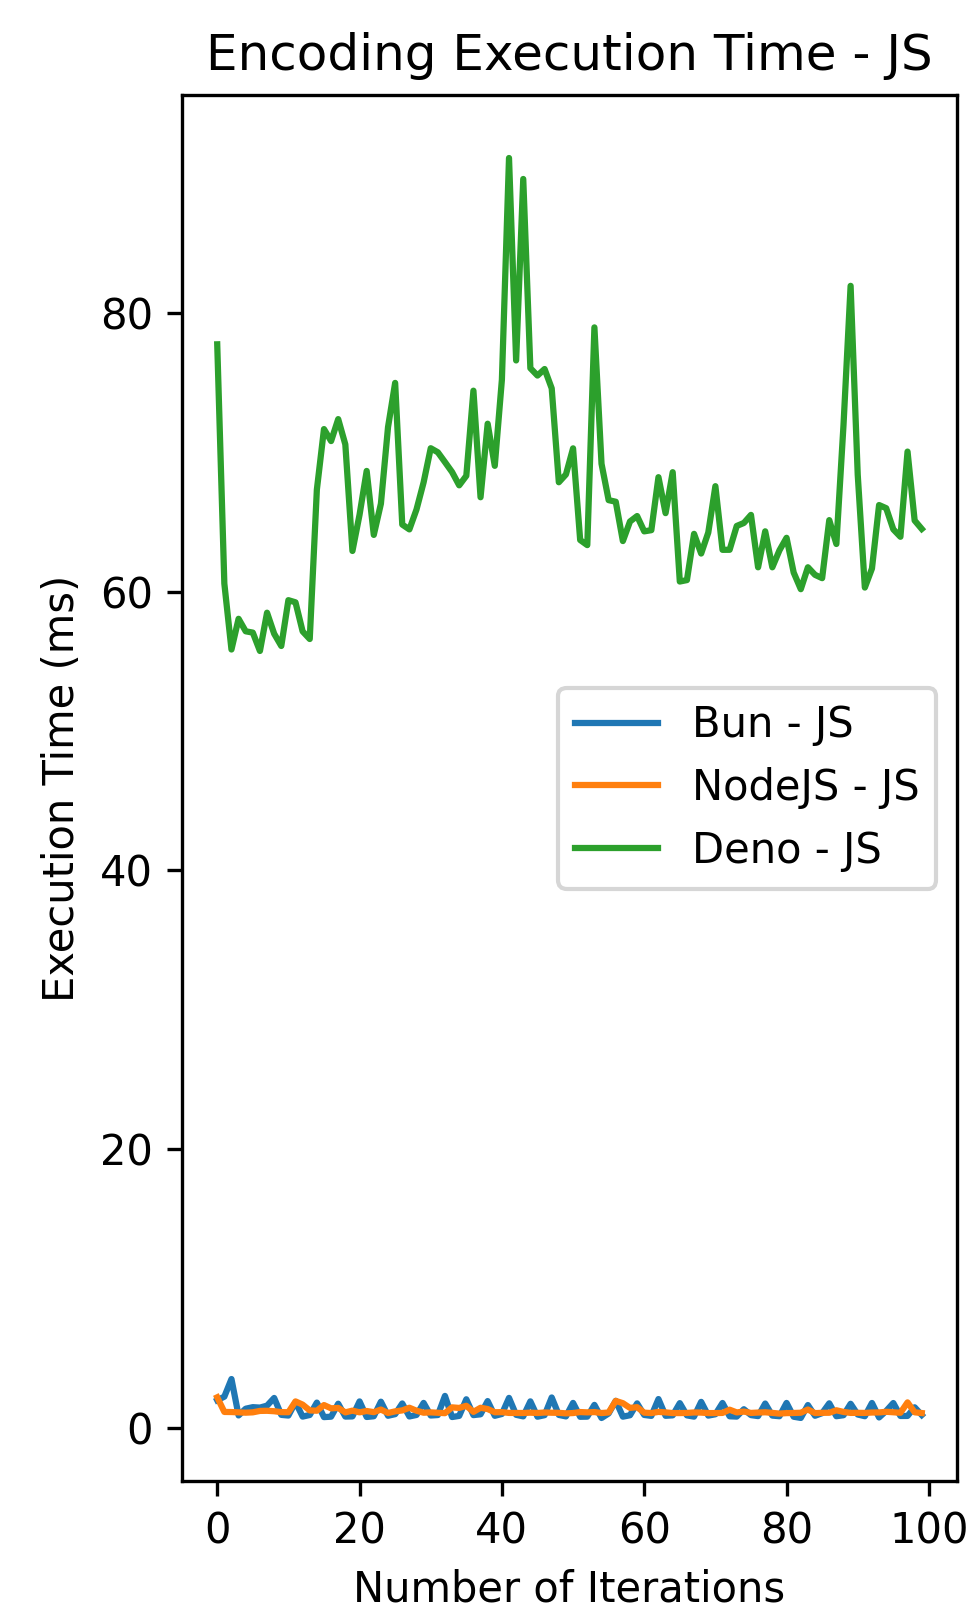
\includegraphics[width=\textwidth]{Figures/coding/base64_100_encoding_js_time.png}
    \caption{Czas wykonania testu w milisekundach (ms)}
    \label{fig:encoding_e1_js_time}
  \end{subfigure}
  \begin{subfigure}[b]{0.42\textwidth}
    \centering
    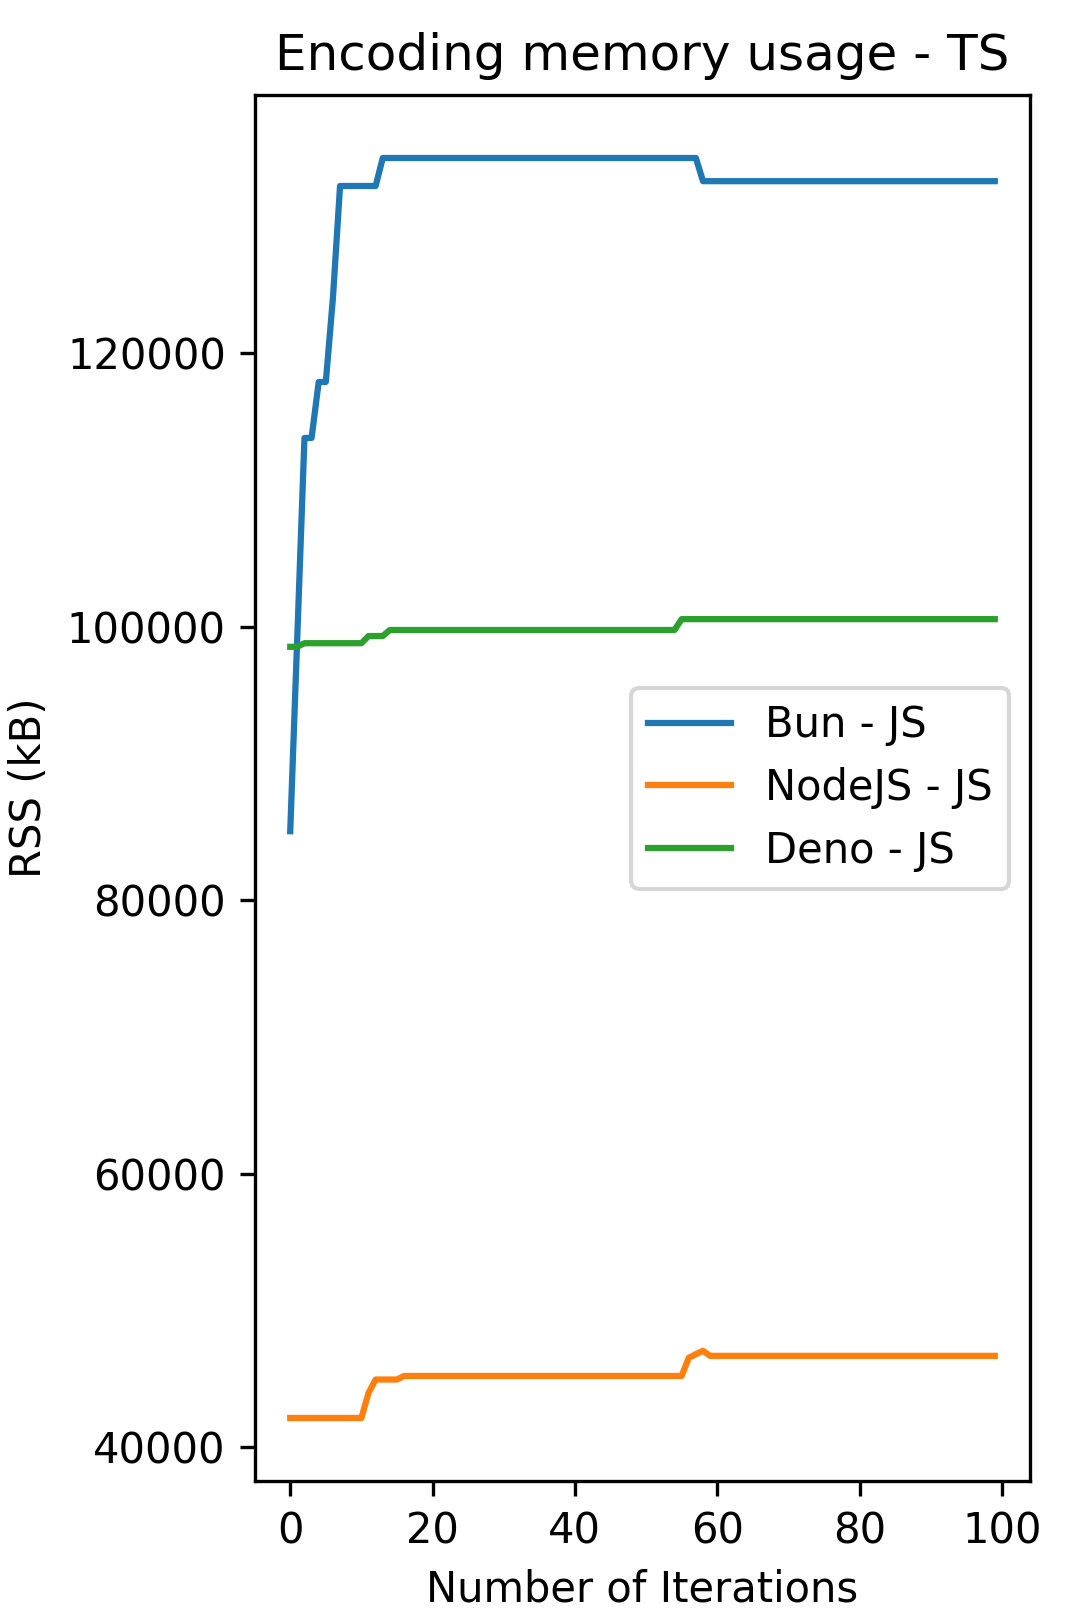
\includegraphics[width=\textwidth]{Figures/coding/base64_100_encoding_js_memory.png}
    \caption{Zużycie pamięci operacyjnej w kilobajtach (kB)}
    \label{fig:encoding_e1_js_memory}
  \end{subfigure}
  \hfill
  \caption{Wyniki eksperymentów dla operacji kodowania z wykorzystaniem algorytmu \textit{Base64} dla 100 iteracji oraz 32768 znaków - a) czas wykonania jednorazowego testu w milisekundach, b) ilość zajmowanej pamięci w kilobajtach (kB)}
  \label{fig:encoding_e1_js}
\end{figure}

Na rysunku \ref{fig:decoding_e1_js} przedstawiono wyniki eksperymentów dla operacji dekodowania z wykorzystaniem kodowania \textit{Base64} dla 100 iteracji i 32768 znaków napisanego w języku JavaScript. Na wykresach przedstawiono czas wykonania jednorazowego testu w milisekundach oraz ilość zajmowanej pamięci w kilobajtach (kB).

\begin{figure}[H]
  \centering
  \begin{subfigure}[b]{0.42\textwidth}
    \centering
    \includegraphics[width=\textwidth]{Figures/coding/base64_100_decoding_js_time.png}
    \caption{Czas wykonania testu w milisekundach (ms)}
    \label{fig:decoding_e1_js_time}
  \end{subfigure}
  \begin{subfigure}[b]{0.42\textwidth}
    \centering
    \includegraphics[width=\textwidth]{Figures/coding/base64_100_decoding_js_memory.png}
    \caption{Zużycie pamięci operacyjnej w kilobajtach (kB)}
    \label{fig:decoding_e1_js_memory}
  \end{subfigure}
  \hfill
  \caption{Wyniki eksperymentów dla operacji dekodowania z wykorzystaniem algorytmu \textit{Base64} dla 100 iteracji oraz 32768 znaków - a) czas wykonania jednorazowego testu w milisekundach, b) ilość zajmowanej pamięci w kilobajtach (kB)}
  \label{fig:decoding_e1_js}
\end{figure}

Na rysunku \ref{fig:encoding_e1_ts} przedstawiono wyniki eksperymentów dla operacji kodowania z wykorzystaniem algorytmu kodowania \textit{Base64} dla 100 iteracji i 32768 znaków napisanego w języku JavaScript. Na wykresach przedstawiono czas wykonania jednorazowego testu w milisekundach oraz ilość zajmowanej pamięci w kilobajtach (kB).

\begin{figure}[H]
  \centering
  \begin{subfigure}[b]{0.42\textwidth}
    \centering
    \includegraphics[width=\textwidth]{Figures/coding/base64_100_decoding_ts_time.png}
    \caption{Czas wykonania testu w milisekundach (ms)}
    \label{fig:encoding_e1_ts_time}
  \end{subfigure}
  \begin{subfigure}[b]{0.42\textwidth}
    \centering
    \includegraphics[width=\textwidth]{Figures/coding/base64_100_decoding_ts_memory.png}
    \caption{Zużycie pamięci operacyjnej w kilobajtach (kB)}
    \label{fig:encoding_e1_ts_memory}
  \end{subfigure}
  \hfill
  \caption{Wyniki eksperymentów dla operacji kodowania z wykorzystaniem algorytmu \textit{Base64} dla 100 iteracji oraz 32768 znaków - a) czas wykonania jednorazowego testu w milisekundach, b) ilość zajmowanej pamięci w kilobajtach (kB)}
  \label{fig:encoding_e1_ts}
\end{figure}

Na rysunku \ref{fig:decoding_e1_ts} przedstawiono wyniki eksperymentów dla operacji dekodowania z wykorzystaniem kodowania \textit{Base64} dla 100 iteracji i 32768 znaków napisanego w języku JavaScript. Na wykresach przedstawiono czas wykonania jednorazowego testu w milisekundach oraz ilość zajmowanej pamięci w kilobajtach (kB).

\begin{figure}[H]
  \centering
  \begin{subfigure}[b]{0.42\textwidth}
    \centering
    \includegraphics[width=\textwidth]{Figures/coding/base64_100_decoding_ts_time.png}
    \caption{Czas wykonania testu w milisekundach (ms)}
    \label{fig:decoding_e1_ts_time}
  \end{subfigure}
  \begin{subfigure}[b]{0.42\textwidth}
    \centering
    \includegraphics[width=\textwidth]{Figures/coding/base64_100_decoding_ts_memory.png}
    \caption{Zużycie pamięci operacyjnej w kilobajtach (kB)}
    \label{fig:decoding_e1_ts_memory}
  \end{subfigure}
  \hfill
  \caption{Wyniki eksperymentów dla operacji dekodowania z wykorzystaniem algorytmu \textit{Base64} dla 100 iteracji oraz 32768 znaków - a) czas wykonania jednorazowego testu w milisekundach, b) ilość zajmowanej pamięci w kilobajtach (kB)}
  \label{fig:decoding_e1_ts}
\end{figure}

Na rysunku \ref{fig:encoding_e2_js} przedstawiono wyniki eksperymentów dla operacji kodowania z wykorzystaniem algorytmu kodowania \textit{Base64} dla 1000 iteracji i 8192 znaków napisanego w języku JavaScript. Na wykresach przedstawiono czas wykonania jednorazowego testu w milisekundach oraz ilość zajmowanej pamięci w kilobajtach (kB).

\begin{figure}[H]
  \centering
  \begin{subfigure}[b]{0.42\textwidth}
    \centering
    \includegraphics[width=\textwidth]{Figures/coding/base64_1000_encoding_js_time.png}
    \caption{Czas wykonania testu w milisekundach (ms)}
    \label{fig:encoding_e2_js_time}
  \end{subfigure}
  \begin{subfigure}[b]{0.42\textwidth}
    \centering
    \includegraphics[width=\textwidth]{Figures/coding/base64_1000_encoding_js_memory.png}
    \caption{Zużycie pamięci operacyjnej w kilobajtach (kB)}
    \label{fig:encoding_e2_js_memory}
  \end{subfigure}
  \hfill
  \caption{Wyniki eksperymentów dla operacji kodowania z wykorzystaniem algorytmu \textit{Base64} dla 1000 iteracji oraz 8192 znaków - a) czas wykonania jednorazowego testu w milisekundach, b) ilość zajmowanej pamięci w kilobajtach (kB)}
  \label{fig:encoding_e2_js}
\end{figure}

Na rysunku \ref{fig:decoding_e2_js} przedstawiono wyniki eksperymentów dla operacji dekodowania z wykorzystaniem kodowania \textit{Base64} dla 1000 iteracji i 8192 znaków napisanego w języku JavaScript. Na wykresach przedstawiono czas wykonania jednorazowego testu w milisekundach oraz ilość zajmowanej pamięci w kilobajtach (kB).

\begin{figure}[H]
  \centering
  \begin{subfigure}[b]{0.42\textwidth}
    \centering
    \includegraphics[width=\textwidth]{Figures/coding/base64_1000_decoding_js_time.png}
    \caption{Czas wykonania testu w milisekundach (ms)}
    \label{fig:decoding_e2_js_time}
  \end{subfigure}
  \begin{subfigure}[b]{0.42\textwidth}
    \centering
    \includegraphics[width=\textwidth]{Figures/coding/base64_1000_decoding_js_memory.png}
    \caption{Zużycie pamięci operacyjnej w kilobajtach (kB)}
    \label{fig:decoding_e2_js_memory}
  \end{subfigure}
  \hfill
  \caption{Wyniki eksperymentów dla operacji dekodowania z wykorzystaniem algorytmu \textit{Base64} dla 1000 iteracji oraz 8192 znaków - a) czas wykonania jednorazowego testu w milisekundach, b) ilość zajmowanej pamięci w kilobajtach (kB)}
  \label{fig:decoding_e2_js}
\end{figure}

Na rysunku \ref{fig:encoding_e2_ts} przedstawiono wyniki eksperymentów dla operacji kodowania z wykorzystaniem algorytmu kodowania \textit{Base64} dla 1000 iteracji i 8192 znaków napisanego w języku JavaScript. Na wykresach przedstawiono czas wykonania jednorazowego testu w milisekundach oraz ilość zajmowanej pamięci w kilobajtach (kB).

\begin{figure}[H]
  \centering
  \begin{subfigure}[b]{0.42\textwidth}
    \centering
    \includegraphics[width=\textwidth]{Figures/coding/base64_1000_encoding_ts_time.png}
    \caption{Czas wykonania testu w milisekundach (ms)}
    \label{fig:encoding_e2_ts_time}
  \end{subfigure}
  \begin{subfigure}[b]{0.42\textwidth}
    \centering
    \includegraphics[width=\textwidth]{Figures/coding/base64_1000_encoding_ts_memory.png}
    \caption{Zużycie pamięci operacyjnej w kilobajtach (kB)}
    \label{fig:encoding_e2_ts_memory}
  \end{subfigure}
  \hfill
  \caption{Wyniki eksperymentów dla operacji kodowania z wykorzystaniem algorytmu \textit{Base64} dla 1000 iteracji oraz 8192 znaków - a) czas wykonania jednorazowego testu w milisekundach, b) ilość zajmowanej pamięci w kilobajtach (kB)}
  \label{fig:encoding_e2_ts}
\end{figure}

Na rysunku \ref{fig:decoding_e2_ts} przedstawiono wyniki eksperymentów dla operacji dekodowania z wykorzystaniem kodowania \textit{Base64} dla 100 iteracji i 8192 znaków napisanego w języku JavaScript. Na wykresach przedstawiono czas wykonania jednorazowego testu w milisekundach oraz ilość zajmowanej pamięci w kilobajtach (kB).

\begin{figure}[H]
  \centering
  \begin{subfigure}[b]{0.42\textwidth}
    \centering
    \includegraphics[width=\textwidth]{Figures/coding/base64_1000_decoding_ts_time.png}
    \caption{Czas wykonania testu w milisekundach (ms)}
    \label{fig:decoding_e2_ts_time}
  \end{subfigure}
  \begin{subfigure}[b]{0.42\textwidth}
    \centering
    \includegraphics[width=\textwidth]{Figures/coding/base64_1000_decoding_ts_memory.png}
    \caption{Zużycie pamięci operacyjnej w kilobajtach (kB)}
    \label{fig:decoding_e2_ts_memory}
  \end{subfigure}
  \hfill
  \caption{Wyniki eksperymentów dla operacji dekodowania z wykorzystaniem algorytmu \textit{Base64} dla 1000 iteracji oraz 8192 znaków - a) czas wykonania jednorazowego testu w milisekundach, b) ilość zajmowanej pamięci w kilobajtach (kB)}
  \label{fig:decoding_e2_ts}
\end{figure}

\subsection{Testy wydajnościowe operacji zapisu i odczytu plików}
W celu zbadania wydajności operacji zapisu oraz odczytu plików, przeprowadzono eksperymenty, które polegały na zapisie oraz odczycie plików o różnych rozmiarach. W przeprowadzonych testach wykorzystano pliki tekstowe, natomiast zawartość plików została wygenerowana za pomocą modułu \textit{faker.js}. W tym celu generowano paragrafy tekstu. W tabeli \ref{tab:file_experiments} przedstawiono liczbę przeprowadzonych eksperymentów oraz rozmiar pliku.

\begin{table}[H]
  \centering
  \caption{Parametry eksperymentów zapisu i odczytu plików}
  \begin{tabular}{|c|c|c|}
    \hline
    \textbf{Ilość eksperymentów} & \textbf{Rozmiar pliku} & \textbf{Ilość plików} \\ \hline
    50 & 512kB & 50 \\ \hline
    50 & 1MB & 50 \\ \hline
  \end{tabular}
  \label{tab:file_experiments}
\end{table}

\subsubsection{Wyniki}
Na rysunku \ref{fig:file_e1_reading_js} przedstawiono wyniki eksperymentów dla operacji zapisu dla 50 iteracji oraz 50 plików o rozmiarze 512kB napisanego w języku JavaScript. Na wykresach przedstawiono czas wykonania jednorazowego testu w milisekundach oraz ilość zajmowanej pamięci w kilobajtach (kB).

\begin{figure}[H]
  \centering
  \begin{subfigure}[b]{0.42\textwidth}
    \centering
    \includegraphics[width=\textwidth]{Figures/files/files_reading_50_500_50_js_time.png}
    \caption{Czas wykonania testu w milisekundach (ms)}
    \label{fig:file_e1_reading_js_time}
  \end{subfigure}
  \begin{subfigure}[b]{0.42\textwidth}
    \centering
    \includegraphics[width=\textwidth]{Figures/files/files_reading_50_500_50_js_memory.png}
    \caption{Zużycie pamięci operacyjnej w kilobajtach (kB)}
    \label{fig:file_e1_reading_js_memory}
  \end{subfigure}
  \caption{Wynik eksperymentów odczytu pliku dla 50 iteracji oraz 50 plików o rozmiarze 512kB - a) czas wykonania jednorazowego testu w milisekundach, b) ilość zajmowanej pamięci w kilobajtach (kB)}
  \label{fig:file_e1_reading_js}
\end{figure}

Na rysunku \ref{fig:file_e1_writing_js} przedstawiono wyniki eksperymentów dla operacji odczytu dla 50 iteracji oraz 50 plików o rozmiarze 512kB napisanego w języku JavaScript. Na wykresach przedstawiono czas wykonania jednorazowego testu w milisekundach oraz ilość zajmowanej pamięci w kilobajtach (kB).

\begin{figure}[H]
  \centering
  \begin{subfigure}[b]{0.42\textwidth}
    \centering
    \includegraphics[width=\textwidth]{Figures/files/files_writing_50_500_50_js_time.png}
    \caption{Czas wykonania testu w milisekundach (ms)}
    \label{fig:file_e1_writing_js_time}
  \end{subfigure}
  \begin{subfigure}[b]{0.42\textwidth}
    \centering
    \includegraphics[width=\textwidth]{Figures/files/files_writing_50_500_50_js_memory.png}
    \caption{Zużycie pamięci operacyjnej w kilobajtach (kB)}
    \label{fig:file_e1_writing_js_memory}
  \end{subfigure}
  \caption{Wynik eksperymentów zapisu pliku dla 50 iteracji oraz 50 plików o rozmiarze 512kB - a) czas wykonania jednorazowego testu w milisekundach, b) ilość zajmowanej pamięci w kilobajtach (kB)}
  \label{fig:file_e1_writing_js}
\end{figure}

Na rysunku \ref{fig:file_e1_reading_ts} przedstawiono wyniki eksperymentów dla operacji zapisu dla 50 iteracji oraz 50 plików o rozmiarze 512kB napisanego w języku TypeScript. Na wykresach przedstawiono czas wykonania jednorazowego testu w milisekundach oraz ilość zajmowanej pamięci w kilobajtach (kB).

\begin{figure}[H]
  \centering
  \begin{subfigure}[b]{0.42\textwidth}
    \centering
    \includegraphics[width=\textwidth]{Figures/files/files_reading_50_500_50_ts_time.png}
    \caption{Czas wykonania testu w milisekundach (ms)}
    \label{fig:file_e1_reading_ts_time}
  \end{subfigure}
  \begin{subfigure}[b]{0.42\textwidth}
    \centering
    \includegraphics[width=\textwidth]{Figures/files/files_reading_50_500_50_ts_memory.png}
    \caption{Zużycie pamięci operacyjnej w kilobajtach (kB)}
    \label{fig:file_e1_reading_ts_memory}
  \end{subfigure}
  \caption{Wynik eksperymentów odczytu pliku dla 50 iteracji oraz 50 plików o rozmiarze 512kB - a) czas wykonania jednorazowego testu w milisekundach, b) ilość zajmowanej pamięci w kilobajtach (kB)}
  \label{fig:file_e1_reading_ts}
\end{figure}

Na rysunku \ref{fig:file_e1_writing_ts} przedstawiono wyniki eksperymentów dla operacji odczytu dla 50 iteracji oraz 50 plików o rozmiarze 512kB napisanego w języku TypeScript. Na wykresach przedstawiono czas wykonania jednorazowego testu w milisekundach oraz ilość zajmowanej pamięci w kilobajtach (kB).

\begin{figure}[H]
  \centering
  \begin{subfigure}[b]{0.42\textwidth}
    \centering
    \includegraphics[width=\textwidth]{Figures/files/files_writing_50_500_50_ts_time.png}
    \caption{Czas wykonania testu w milisekundach (ms)}
    \label{fig:file_e1_writing_ts_time}
  \end{subfigure}
  \begin{subfigure}[b]{0.42\textwidth}
    \centering
    \includegraphics[width=\textwidth]{Figures/files/files_writing_50_500_50_ts_memory.png}
    \caption{Zużycie pamięci operacyjnej w kilobajtach (kB)}
    \label{fig:file_e1_writing_ts_memory}
  \end{subfigure}
  \caption{Wynik eksperymentów zapisu pliku dla 50 iteracji oraz 50 plików o rozmiarze 512kB - a) czas wykonania jednorazowego testu w milisekundach, b) ilość zajmowanej pamięci w kilobajtach (kB)}
  \label{fig:file_e1_writing_ts}
\end{figure}

Na rysunku \ref{fig:file_e2_reading_js} przedstawiono wyniki eksperymentów dla operacji zapisu dla 50 iteracji oraz 50 plików o rozmiarze 1MB napisanego w języku JavaScript. Na wykresach przedstawiono czas wykonania jednorazowego testu w milisekundach oraz ilość zajmowanej pamięci w kilobajtach (kB).

\begin{figure}[H]
  \centering
  \begin{subfigure}[b]{0.42\textwidth}
    \centering
    \includegraphics[width=\textwidth]{Figures/files/files_reading_50_2000_50_js_time.png}
    \caption{Czas wykonania testu w milisekundach (ms)}
    \label{fig:file_e2_reading_js_time}
  \end{subfigure}
  \begin{subfigure}[b]{0.42\textwidth}
    \centering
    \includegraphics[width=\textwidth]{Figures/files/files_reading_50_2000_50_js_memory.png}
    \caption{Zużycie pamięci operacyjnej w kilobajtach (kB)}
    \label{fig:file_e2_reading_js_memory}
  \end{subfigure}
  \caption{Wynik eksperymentów odczytu pliku dla 50 iteracji oraz 50 plików o rozmiarze 1MB - a) czas wykonania jednorazowego testu w milisekundach, b) ilość zajmowanej pamięci w kilobajtach (kB)}
  \label{fig:file_e2_reading_js}
\end{figure}

Na rysunku \ref{fig:file_e2_writing_js} przedstawiono wyniki eksperymentów dla operacji odczytu dla 50 iteracji oraz 50 plików o rozmiarze 1MB napisanego w języku JavaScript. Na wykresach przedstawiono czas wykonania jednorazowego testu w milisekundach oraz ilość zajmowanej pamięci w kilobajtach (kB).

\begin{figure}[H]
  \centering
  \begin{subfigure}[b]{0.42\textwidth}
    \centering
    \includegraphics[width=\textwidth]{Figures/files/files_writing_50_2000_50_js_time.png}
    \caption{Czas wykonania testu w milisekundach (ms)}
    \label{fig:file_e2_writing_js_time}
  \end{subfigure}
  \begin{subfigure}[b]{0.42\textwidth}
    \centering
    \includegraphics[width=\textwidth]{Figures/files/files_writing_50_2000_50_js_memory.png}
    \caption{Zużycie pamięci operacyjnej w kilobajtach (kB)}
    \label{fig:file_e2_writing_js_memory}
  \end{subfigure}
  \caption{Wynik eksperymentów zapisu pliku dla 50 iteracji oraz 50 plików o rozmiarze 1MB - a) czas wykonania jednorazowego testu w milisekundach, b) ilość zajmowanej pamięci w kilobajtach (kB)}
  \label{fig:file_e2_writing_js}
\end{figure}

Na rysunku \ref{fig:file_e2_reading_ts} przedstawiono wyniki eksperymentów dla operacji zapisu dla 50 iteracji oraz 50 plików o rozmiarze 1MB napisanego w języku TypeScript. Na wykresach przedstawiono czas wykonania jednorazowego testu w milisekundach oraz ilość zajmowanej pamięci w kilobajtach (kB).

\begin{figure}[H]
  \centering
  \begin{subfigure}[b]{0.42\textwidth}
    \centering
    \includegraphics[width=\textwidth]{Figures/files/files_reading_50_2000_50_ts_time.png}
    \caption{Czas wykonania testu w milisekundach (ms)}
    \label{fig:file_e2_reading_ts_time}
  \end{subfigure}
  \begin{subfigure}[b]{0.42\textwidth}
    \centering
    \includegraphics[width=\textwidth]{Figures/files/files_reading_50_2000_50_ts_memory.png}
    \caption{Zużycie pamięci operacyjnej w kilobajtach (kB)}
    \label{fig:file_e2_reading_ts_memory}
  \end{subfigure}
  \caption{Wynik eksperymentów odczytu pliku dla 50 iteracji oraz 50 plików o rozmiarze 1MB - a) czas wykonania jednorazowego testu w milisekundach, b) ilość zajmowanej pamięci w kilobajtach (kB)}
  \label{fig:file_e2_reading_ts}
\end{figure}

Na rysunku \ref{fig:file_e2_writing_ts} przedstawiono wyniki eksperymentów dla operacji odczytu dla 50 iteracji oraz 50 plików o rozmiarze 1MB napisanego w języku TypeScript. Na wykresach przedstawiono czas wykonania jednorazowego testu w milisekundach oraz ilość zajmowanej pamięci w kilobajtach (kB).

\begin{figure}[H]
  \centering
  \begin{subfigure}[b]{0.42\textwidth}
    \centering
    \includegraphics[width=\textwidth]{Figures/files/files_writing_50_2000_50_ts_time.png}
    \caption{Czas wykonania testu w milisekundach (ms)}
    \label{fig:file_e2_writing_ts_time}
  \end{subfigure}
  \begin{subfigure}[b]{0.42\textwidth}
    \centering
    \includegraphics[width=\textwidth]{Figures/files/files_writing_50_2000_50_ts_memory.png}
    \caption{Zużycie pamięci operacyjnej w kilobajtach (kB)}
    \label{fig:file_e2_writing_ts_memory}
  \end{subfigure}
  \caption{Wynik eksperymentów zapisu pliku dla 50 iteracji oraz 50 plików o rozmiarze 1MB - a) czas wykonania jednorazowego testu w milisekundach, b) ilość zajmowanej pamięci w kilobajtach (kB)}
  \label{fig:file_e2_writing_ts}
\end{figure}

\subsection{Testy wydajnościowe serwera HTTP}
W celu zbadania wydajności serwera HTTP, przeprowadzono testy obciążeniowe. Do testów została wykorzystany program \textit{oha} \cite{oha}, który pozwala na połączenie się do serwera HTTP oraz wysyłanie żądań z kilku połączeń jednocześnie. W tabeli \ref{tab:http_experiments} przedstawiono liczbę przeprowadzonych eksperymentów oraz ilość połączeń.

\begin{table}[H]
  \centering
  \caption{Parametry eksperymentów serwera HTTP}
  \begin{tabular}{|c|c|}
    \hline
    \textbf{Liczba żądań} & \textbf{Liczba połączeń}\\ \hline
    10000 & 100 \\ \hline
    10000 & 1000 \\ \hline
    10000 & 10000 \\ \hline
  \end{tabular}
  \label{tab:http_experiments}
\end{table}

\subsubsection{Wyniki}
Na rysunku \ref{fig:server_e1} przedstawiono wyniki eksperymentów dla testu wydajnościowego serwera HTTP dla 100 równoczesnych połączeń oraz 10000 żądań HTTP. Wyniki zostały przedstawione zarówno dla języka JavaScript oraz TypeScript. Na wykresach przedstawiono wynik testu obciążeniowego wyrażonego w RPS (\textit{Request per second}).

\begin{figure}[H]
  \centering
  \begin{subfigure}[b]{0.42\textwidth}
    \centering
    \includegraphics[width=\textwidth]{Figures/server/server_100_10000_js.png}
    \caption{Czas wykonania testu w milisekundach (ms)}
    \label{fig:server_e1_js}
  \end{subfigure}
  \begin{subfigure}[b]{0.42\textwidth}
    \centering
    \includegraphics[width=\textwidth]{Figures/server/server_100_10000_ts.png}
    \caption{Wynik testu obciążeniowego wyrażonego w RPS (\textit{Request per second}}
    \label{fig:server_e1_ts}
  \end{subfigure}
  \caption{Wynik eksperymentów dla testu obciążeniowego serwera HTTP 100 równoczesnych połączeń oraz 10000 żądań HTTP, wyrażonego w RPS (\textit{Request per second}) - a) dla języka JavaScript, b) dla języka TypeScript}
  \label{fig:server_e1}
\end{figure}

Na rysunku \ref{fig:server_e2} przedstawiono wyniki eksperymentów dla testu wydajnościowego serwera HTTP dla 1000 równoczesnych połączeń oraz 10000 żądań HTTP. Wyniki zostały przedstawione zarówno dla języka JavaScript oraz TypeScript. Na wykresach przedstawiono wynik testu obciążeniowego wyrażonego w RPS (\textit{Request per second}).

\begin{figure}[H]
  \centering
  \begin{subfigure}[b]{0.42\textwidth}
    \centering
    \includegraphics[width=\textwidth]{Figures/server/server_1000_10000_js.png}
    \caption{Wynik testu obciążeniowego wyrażonego w RPS (\textit{Request per second}) dla języka JavaScript}
    \label{fig:server_e2_js}
  \end{subfigure}
  \begin{subfigure}[b]{0.42\textwidth}
    \centering
    \includegraphics[width=\textwidth]{Figures/server/server_1000_10000_ts.png}
    \caption{Wynik testu obciążeniowego wyrażonego w RPS (\textit{Request per second}) dla języka TypeScript}
    \label{fig:server_e2_ts}
  \end{subfigure}
  \caption{Wynik eksperymentów dla testu obciążeniowego serwera HTTP 1000 równoczesnych połączeń oraz 10000 żądań HTTP, wyrażonego w RPS (\textit{Request per second}) - a) dla języka JavaScript, b) dla języka TypeScript}
  \label{fig:server_e2}
\end{figure}

Na rysunku \ref{fig:server_e3} przedstawiono wyniki eksperymentów dla testu wydajnościowego serwera HTTP dla 10000 równoczesnych połączeń oraz 10000 żądań HTTP. Wyniki zostały przedstawione zarówno dla języka JavaScript oraz TypeScript. Na wykresach przedstawiono wynik testu obciążeniowego wyrażonego w RPS (\textit{Request per second}).

\begin{figure}[H]
  \centering
  \begin{subfigure}[b]{0.42\textwidth}
    \centering
    \includegraphics[width=\textwidth]{Figures/server/server_10000_10000_js.png}
    \caption{Wynik testu obciążeniowego wyrażonego w RPS (\textit{Request per second}) dla języka JavaScript}
    \label{fig:server_e3_js}
  \end{subfigure}
  \begin{subfigure}[b]{0.42\textwidth}
    \centering
    \includegraphics[width=\textwidth]{Figures/server/server_10000_10000_ts.png}
    \caption{Wynik testu obciążeniowego wyrażonego w RPS (\textit{Request per second}) dla języka TypeScript}
    \label{fig:server_e3_ts}
  \end{subfigure}
  \caption{Wynik eksperymentów dla testu obciążeniowego serwera HTTP 10000 równoczesnych połączeń oraz 10000 żądań HTTP, wyrażonego w RPS (\textit{Request per second}) - a) dla języka JavaScript, b) dla języka TypeScript}
  \label{fig:server_e3}
\end{figure}

\subsection{Testy wydajnościowe zapisu i odczytu danych z bazy danych}
W celu zbadania wydajności operacji zapisu oraz odczytu danych z bazy danych, przeprowadzono testy wydajnościowe z wykorzystaniem bazy danych SQLite. W celu wygenerowania danych do bazy danych, wykorzystano moduł \textit{faker.js}. W tabeli \ref{tab:database_experiments} przedstawiono liczbę przeprowadzonych eksperymentów oraz ilość rekordów.

\begin{table}[H]
  \centering
  \caption{Parametry eksperymentów zapisu i odczytu danych z bazy danych}
  \begin{tabular}{|c|c|}
    \hline
    \textbf{Liczba eksperymentów} & \textbf{Liczba rekordów}\\ \hline
    10 & 1000 \\ \hline
    100 & 1000 \\ \hline
  \end{tabular}
  \label{tab:database_experiments}
\end{table}

\subsubsection{Wyniki}
Na rysunku \ref{fig:database_e1_js} przedstawiono wyniki eksperymentów dla testu bazy danych dla 10 iteracji oraz 1000 rekordów napisanego w języku JavaScript. Na wykresach przedstawiono czas wykonania jednorazowego testu w milisekundach oraz ilość zajmowanej pamięci w kilobajtach (kB).

\begin{figure}[H]
  \centering
  \begin{subfigure}[b]{0.42\textwidth}
    \centering
    \includegraphics[width=\textwidth]{Figures/database/sqlite_10_1000_js_time.png}
    \caption{Czas wykonania testu w milisekundach (ms)}
    \label{fig:database_e1_js_time}
  \end{subfigure}
  \begin{subfigure}[b]{0.42\textwidth}
    \centering
    \includegraphics[width=\textwidth]{Figures/database/sqlite_10_1000_js_memory.png}
    \caption{Zużycie pamięci operacyjnej w kilobajtach (kB)}
    \label{fig:database_e1_js_memory}
  \end{subfigure}
  \caption{Wyniki eksperymentów dla testu bazy danych 10 iteracji oraz 1000 rekordów - po lewej czas wykonania jednorazowego testu w milisekundach, po prawej ilość zajmowanej pamięci w kilobajtach (kB)}
  \label{fig:database_e1_js}
\end{figure}

Na rysunku \ref{fig:database_e1_ts} przedstawiono wyniki eksperymentów dla testu bazy danych dla 10 iteracji oraz 1000 rekordów napisanego w języku TypeScript. Na wykresach przedstawiono czas wykonania jednorazowego testu w milisekundach oraz ilość zajmowanej pamięci w kilobajtach (kB).

\begin{figure}[H]
  \centering
  \begin{subfigure}[b]{0.42\textwidth}
    \centering
    \includegraphics[width=\textwidth]{Figures/database/sqlite_10_1000_ts_time.png}
    \caption{Czas wykonania testu w milisekundach (ms)}
    \label{fig:database_e1_ts_time}
  \end{subfigure}
  \begin{subfigure}[b]{0.42\textwidth}
    \centering
    \includegraphics[width=\textwidth]{Figures/database/sqlite_10_1000_ts_memory.png}
    \caption{Zużycie pamięci operacyjnej w kilobajtach (kB)}
    \label{fig:database_e1_ts_memory}
  \end{subfigure}
  \caption{Wyniki eksperymentów dla testu bazy danych 10 iteracji oraz 1000 rekordów - po lewej czas wykonania jednorazowego testu w milisekundach, po prawej ilość zajmowanej pamięci w kilobajtach (kB)}
  \label{fig:database_e1_ts}
\end{figure}

Na rysunku \ref{fig:database_e2_js} przedstawiono wyniki eksperymentów dla testu bazy danych dla 100 iteracji oraz 1000 rekordów napisanego w języku JavaScript. Na wykresach przedstawiono czas wykonania jednorazowego testu w milisekundach oraz ilość zajmowanej pamięci w kilobajtach (kB).

\begin{figure}[H]
  \centering
  \begin{subfigure}[b]{0.42\textwidth}
    \centering
    \includegraphics[width=\textwidth]{Figures/database/sqlite_100_1000_js_time.png}
    \caption{Czas wykonania testu w milisekundach (ms)}
    \label{fig:database_e2_js_time}
  \end{subfigure}
  \begin{subfigure}[b]{0.42\textwidth}
    \centering
    \includegraphics[width=\textwidth]{Figures/database/sqlite_100_1000_js_memory.png}
    \caption{Zużycie pamięci operacyjnej w kilobajtach (kB)}
    \label{fig:database_e2_js_memory}
  \end{subfigure}
  \caption{Wyniki eksperymentów dla testu bazy danych 10 iteracji oraz 1000 rekordów - po lewej czas wykonania jednorazowego testu w milisekundach, po prawej ilość zajmowanej pamięci w kilobajtach (kB)}
  \label{fig:database_e2_js}
\end{figure}

Na rysunku \ref{fig:database_e2_ts} przedstawiono wyniki eksperymentów dla testu bazy danych dla 100 iteracji oraz 1000 rekordów napisanego w języku TypeScript. Na wykresach przedstawiono czas wykonania jednorazowego testu w milisekundach oraz ilość zajmowanej pamięci w kilobajtach (kB).

\begin{figure}[H]
  \centering
  \begin{subfigure}[b]{0.42\textwidth}
    \centering
    \includegraphics[width=\textwidth]{Figures/database/sqlite_100_1000_ts_time.png}
    \caption{Czas wykonania testu w milisekundach (ms)}
    \label{fig:database_e2_ts_time}
  \end{subfigure}
  \begin{subfigure}[b]{0.42\textwidth}
    \centering
    \includegraphics[width=\textwidth]{Figures/database/sqlite_100_1000_ts_memory.png}
    \caption{Zużycie pamięci operacyjnej w kilobajtach (kB)}
    \label{fig:database_e2_ts_memory}
  \end{subfigure}
  \caption{Wyniki eksperymentów dla testu bazy danych 10 iteracji oraz 1000 rekordów - po lewej czas wykonania jednorazowego testu w milisekundach, po prawej ilość zajmowanej pamięci w kilobajtach (kB)}
  \label{fig:database_e2_ts}
\end{figure}